Di seguito verranno illustrate e analizzate diverse implementazioni del filtro FIR. In particolare, verranno mostrati i report generati da HLS e Vivado così da effettuare ulteriori considerazioni a riguardo. Bisogna precisare che la prima soluzione presentata, cioè quella iniziale non ottimizzata, verrà discussa approfonditamente così da affrontare e spiegare i parametri di confronto che verranno utilizzati nelle successive sezioni.

\subsection{Unoptimized Solution}
Qui di seguito viene riportato il codice relativo alla soluzione iniziale (non ottimizzata) del fitro FIR in questione.

\lstinputlisting[language=C++]{solutions/unoptimized/fir_unoptimized.cpp}

In particolare, si può notare come l'input, l'output e i coefficienti utilizzati risultano essere definiti rispettivamente tramite i tipi \textit{samplesType}, \textit{samplesType} e \textit{coeffsType}, cioè tutti e tre definiti come tipi di dato \textit{int} come descritto in \textit{definitions.h}. 
Bisogna specificare che l'operazione di convoluzione è stata ottenuta mediante il loop qui sopra definito. Tale operazione è data dallo shifting dei valori di input al filtro e, successivamente, dall'accumulo. Quest'ultimo è ottenuto mediante la somma, tra la corrente calcolata e la precedente accumulata, e il prodotto, tra il valore shiftato nella precedente iterazione e il coefficiente \textit{i-esimo} corrispondente.\\
Infine, il valore accumulato nella variabile \textit{accumulator} viene assegnato all'output atteso dalla procedura.\\
Effettuando la sintesi è possibile evidenziare il seguente report:\\

\begin{table}[H]
    \centering
    \begin{minipage}[t]{0.45\linewidth}
        \centering
        \begin{tabular}{|c|c|c|c|}
            \hline
            \textbf{Clock} & \textbf{Target} & \textbf{Estimated} & \textbf{Uncertainty} \\
            \hline
            ap\_clk & 10.00 & 8.510 & 1.25 \\
            \hline
        \end{tabular}
        \caption{HLS Unoptimized Solution Timing Summary (ns)}
        \label{tab:hls-unoptimized-solution-timing-summary}
    \end{minipage}
    \hfill
    \begin{minipage}[t]{0.45\linewidth}
        \centering
        \begin{tabular}{|c|c|c|c|}
            \hline
            \multicolumn{2}{|c|}{\textbf{Latency}} & \multicolumn{2}{|c|}{\textbf{Interval}} \\
            min & max & min & max \\
            \hline
            23 & 45 & 23 & 45 \\
            \hline
        \end{tabular}
        \caption{HLS Unoptimized Solution Latency Summary (clock cycles)}
        \label{tab:hls-unoptimized-solution-latency-summary}
    \end{minipage}
\end{table}

Si può notare come il periodo di clock previsto è pari a 10 ns, come impostato durante la creazione della solution in questione, mentre quello stimato è minore. Questo è dovuto al fatto che il tool stima un'incertezza (assimilabile ad un margine) che permette di calcolare il periodo di clock effettivo utilizzato dal processo di sintesi.
\begin{figure}[H]
    \centering
    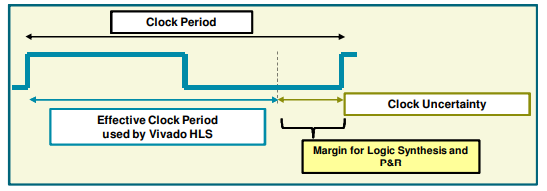
\includegraphics[width=0.5\textwidth]{solutions/unoptimized/clockperiod.png}
    \caption{HLS Clock Period from Synthesis Report}
\end{figure}

In particolare, il periodo di clock effettivo, calcolato dal tool, non deve essere considerato come parametro di progettazione ma come un margine di sicurezza previsto da HLS per il successivo place and route. Nel caso in cui si volesse operare sul periodo di clock della solution come design parameter, si dovrebbe impostare un periodo di clock differente durante la creazione della solution e poi far calcolare automaticamente l'incertezza ed il periodo del clock effettivo dallo stesso tool.

\begin{table}[H]
    \centering
    \begin{tabular}{|c|c|c|c|c|c|c|c|}
        \hline
        \multicolumn{1}{|c|}{Loop} & \multicolumn{2}{|c|}{\textbf{Latency}} & \multicolumn{1}{c|}{\textbf{Iteration Latency}} & \multicolumn{2}{c|}{\textbf{Initiation Interval}} & \multicolumn{1}{c|}{\textbf{Trip Count}}  \\
        Name & min & max &  & achieved & target &  \\
        \hline
        - loop & 22 & 44 & 2$\sim$4 & - & - & 11 \\
        \hline
    \end{tabular}
    \caption{HLS Unoptimized Solution Latency Loops Summary }
    \label{tab:hls-unoptimized-solution-loop-summary}
\end{table}

Considerando, invece, il loop descritto nel file sorgente, si può notare come esso presenti 11 iterazioni (corrispondenti alla capienza di processing del filtro corrispondente) e una iteration latency (IL), cioè latenza per ogni iterazione, compresa tra 2 e 4 cicli di clock. Si deduce che la latenza totale del loop in questione sia compresa tra 22 e 44 cicli di clock.
\begin{figure}[H]
    \centering
    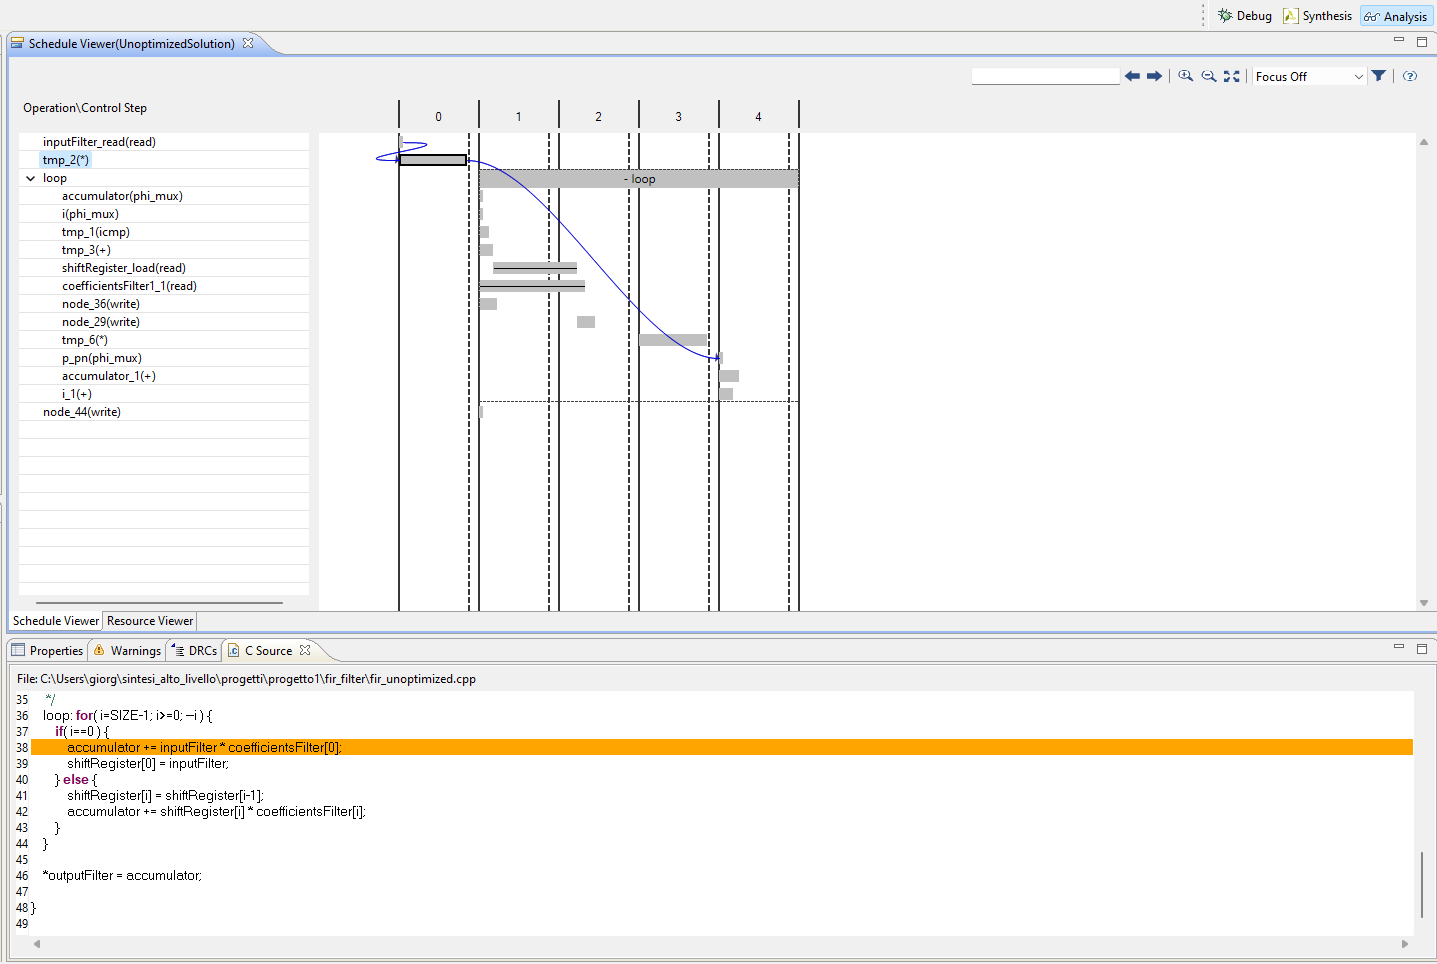
\includegraphics[width=0.7\textwidth]{solutions/unoptimized/cyclesunoptimized.png}
    \caption{HLS Unoptimized Solution If Statement Analysis}
\end{figure}

In particolare, si può notare come il ciclo di clock in più, previsto nella latenza totale dell'architettura, sia dovuto alla verifica dell'istruzione condizionale, al calcolo dell'accumulo e all'assegnazione in corrispondenza dell'iterazione 0 all'interno del loop. È come se l'if all'interno del ciclo for venga trattato al di fuori dello stesso loop. Questo può essere notato facendo riferimento alle operazioni svolte all'interno del loop.

Inoltre, si può notare come le operazioni di lettura previste all'interno del loop siano svolte in parallelo (come mostrato nel primo gruppo di figure allegato), mentre quelle di scrittura schedulate in differente maniera (come mostrato nel secondo gruppo di figure allegato).
\begin{figure}[H]
    \centering
    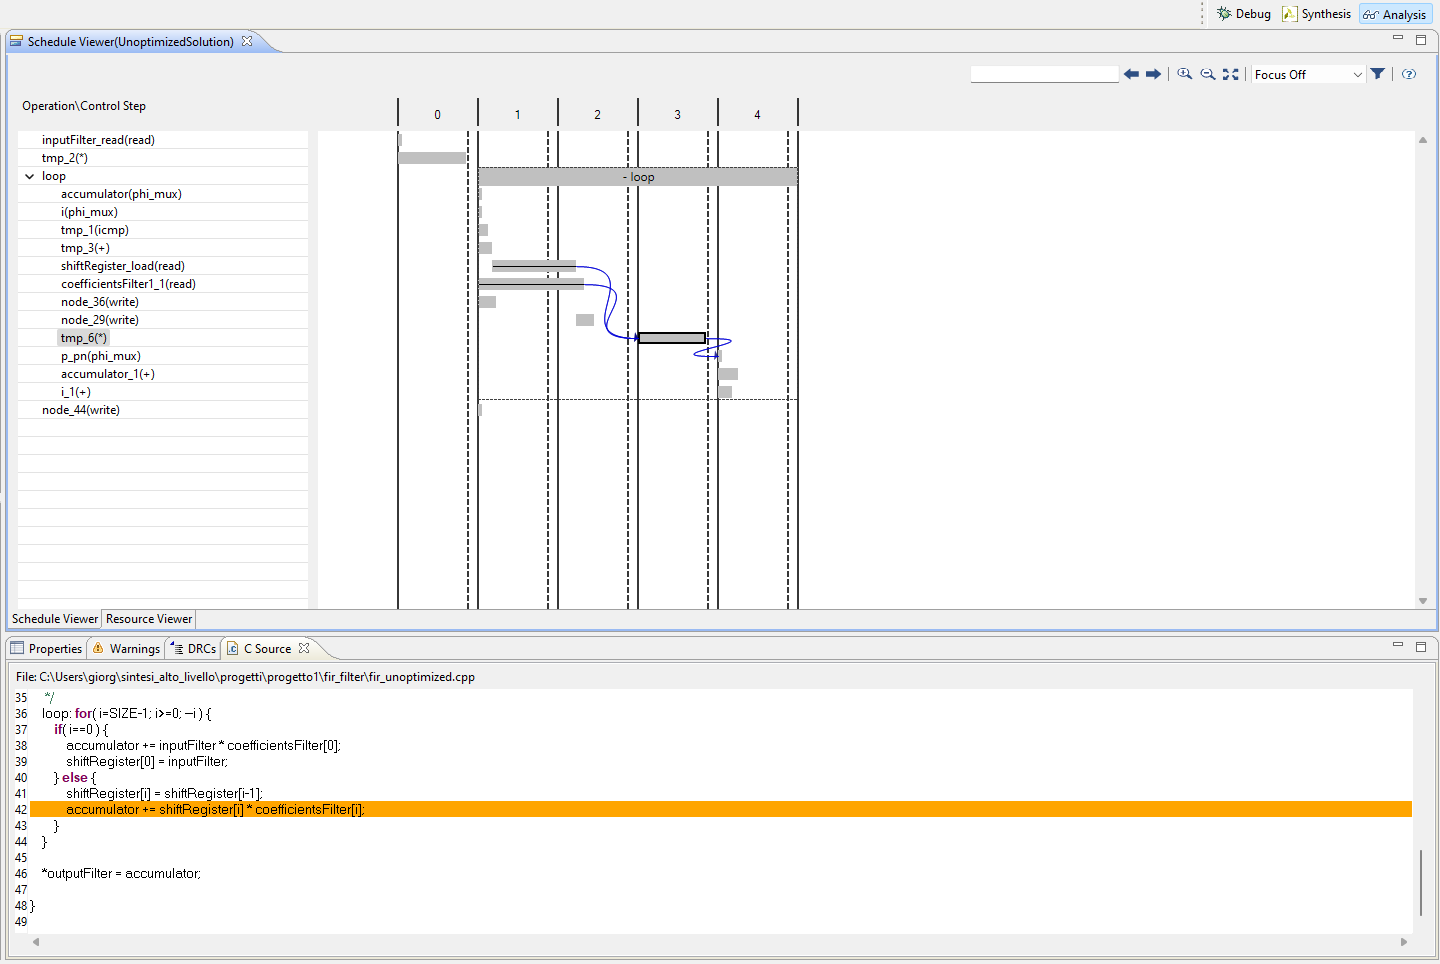
\includegraphics[width=0.7\textwidth]{solutions/unoptimized/cyclesunoptimized2.png}
    \caption{HLS Unoptimized Solution Else Statement Analysis}
\end{figure}

Infatti, si può notare come la latenza associata alle operazioni previste nelle rimanenti iterazioni del loop venga correlata alla latency associata al ciclo stesso.
\begin{figure}[H]
    \centering
    \begin{minipage}[b]{0.45\textwidth}
        \centering
        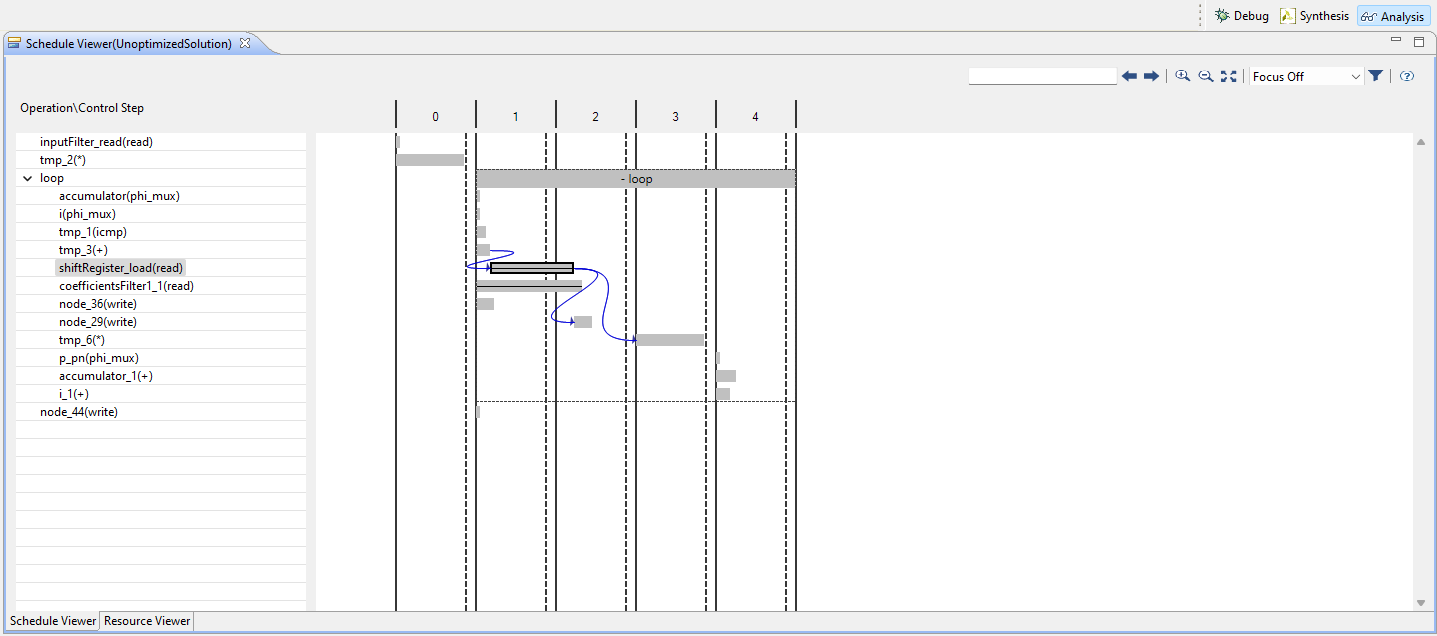
\includegraphics[width=\textwidth]{solutions/unoptimized/cyclesunoptimized3.png}
        \caption{HLS Unoptimized Solution Read Operations Analysis}
        \label{fig:left}
    \end{minipage}
    \hfill
    \begin{minipage}[b]{0.45\textwidth}
        \centering
        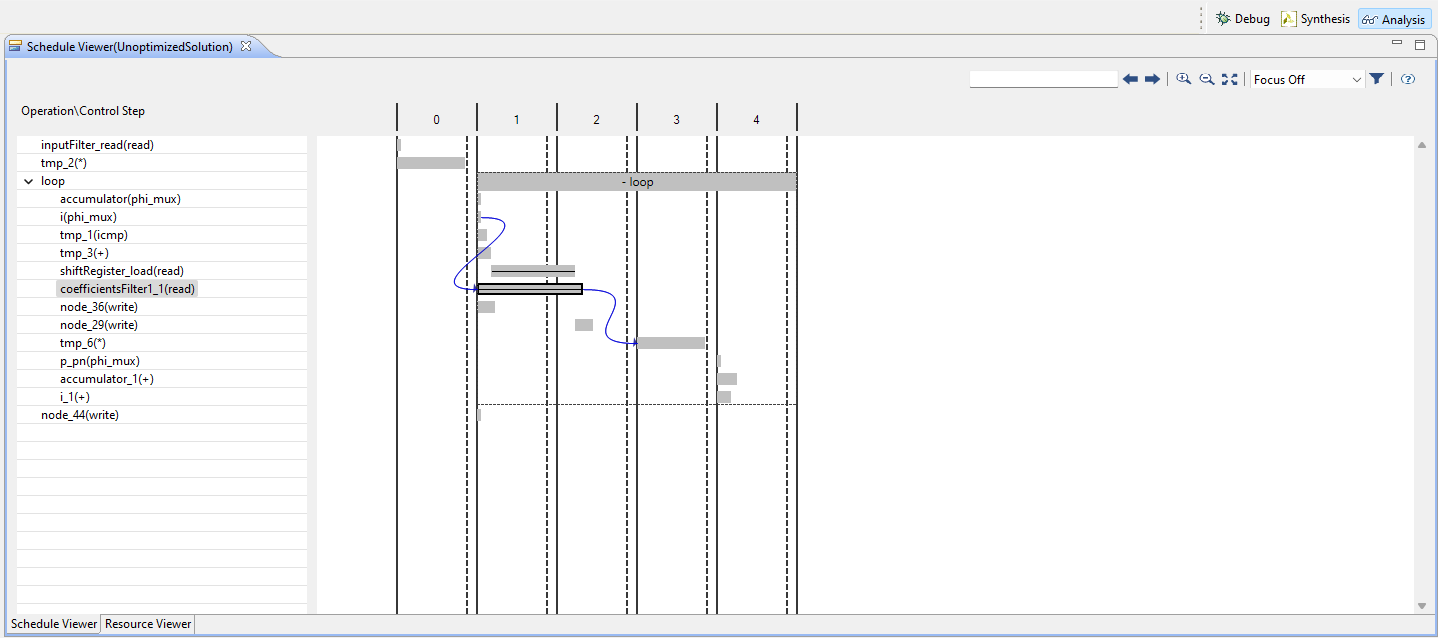
\includegraphics[width=\textwidth]{solutions/unoptimized/cyclesunoptimized4.png}
        \caption{HLS Unoptimized Solution Read Operations Analysis}
        \label{fig:right}
    \end{minipage}
\end{figure}
\begin{figure}[H]
    \centering
    \begin{minipage}[b]{0.45\textwidth}
        \centering
        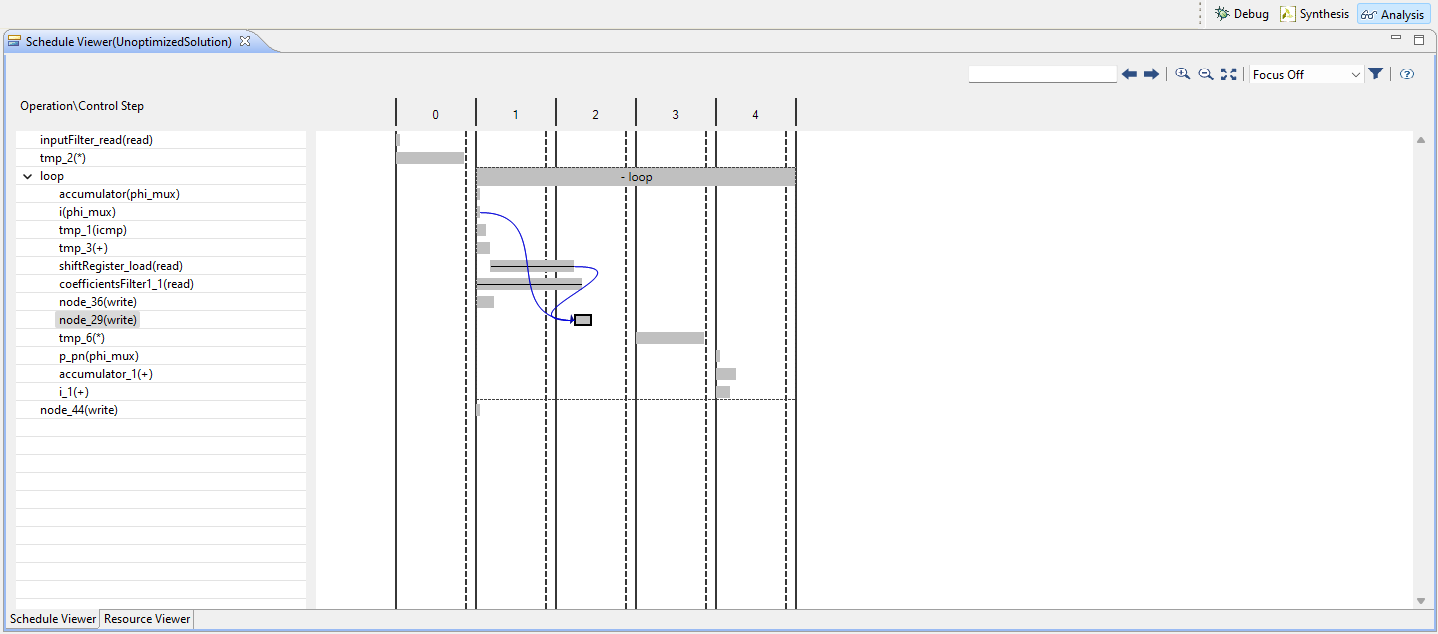
\includegraphics[width=\textwidth]{solutions/unoptimized/cyclesunoptimized5.png}
        \caption{HLS Unoptimized Solution Write Operations Analysis}
        \label{fig:left}
    \end{minipage}
    \hfill
    \begin{minipage}[b]{0.45\textwidth}
        \centering
        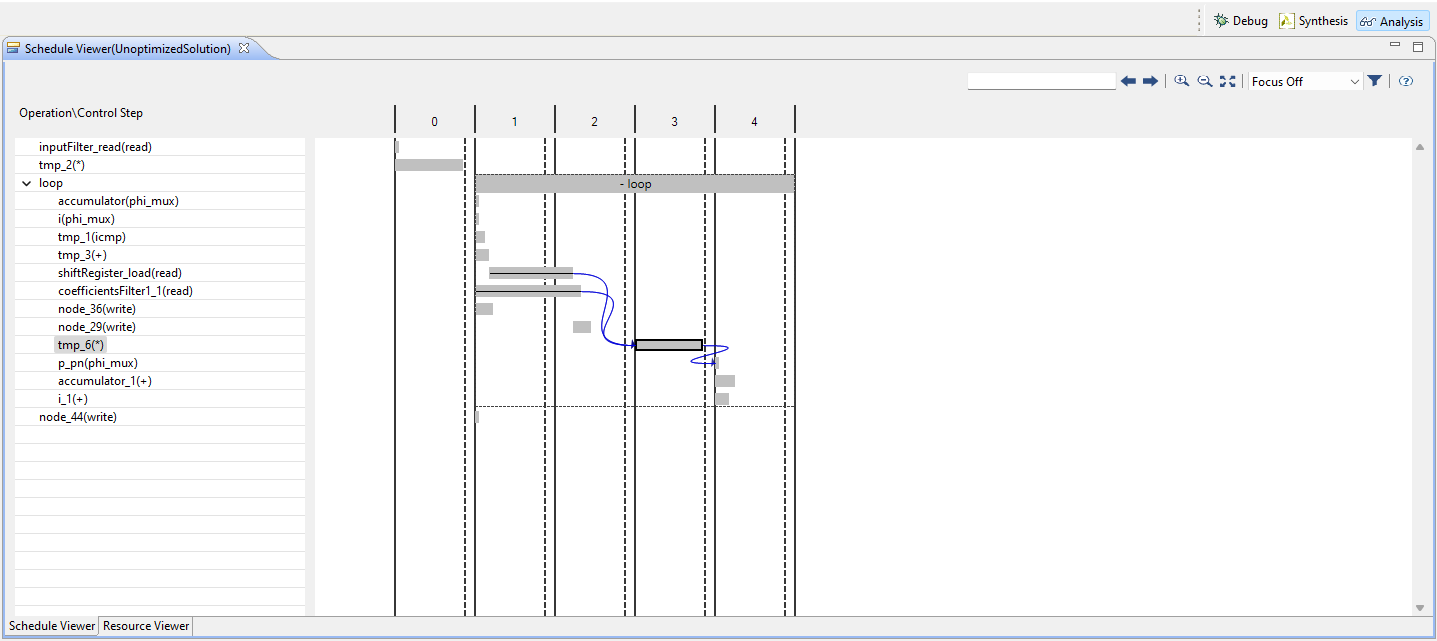
\includegraphics[width=\textwidth]{solutions/unoptimized/cyclesunoptimized6.png}
        \caption{HLS Unoptimized Solution Write Operations Analysis}
        \label{fig:right}
    \end{minipage}
\end{figure}

Qui di seguito, viene allegato l'utilizzazione delle risorse stimata dal processo di sintesi.
\begin{table}[h]
    \centering
    \begin{tabular}{|l|c|c|c|c|}
        \hline
        \textbf{Name}    & \textbf{BRAM\_18K} & \textbf{DSP48E} & \textbf{FF} & \textbf{LUT} \\ \hline
        DSP              & -                   & -               & -           & -            \\ 
        Expression       & -                   & 4               & 0           & 105          \\ 
        FIFO             & -                   & -               & -           & -            \\ 
        Instance         & -                   & -               & -           & -            \\ 
        Memory           & 0                   & -               & 74          & 8            \\ 
        Multiplexer      & -                   & -               & -           & 120          \\ 
        Register         & -                   & -               & 213         & -            \\ \hline
        \textbf{Total}   & 0                   & 4               & 287         & 233          \\ \hline
        \textbf{Available} & 280               & 220             & 106400      & 53200        \\ \hline
        \textbf{Utilization (\%)} & 0            & 1               & $\sim$0     & $\sim$0      \\ \hline
    \end{tabular}
    \caption{HLS Unoptimized Solution Utilization Estimates Summary}
    \label{tab:hls-unoptimized-solution-utilization-estimates-summary}
\end{table}

Successivamente effettuando la C/RTL Cosimulation è possibile evidenziare il seguente report:
\begin{table}[H]
    \centering
    \begin{tabular}{|c|c|c|c|c|c|c|c|}
        \hline
        \multicolumn{1}{|c|}{RTL} & \multicolumn{1}{|c|}{Status} & \multicolumn{3}{c|}{\textbf{Latency}} & \multicolumn{3}{c|}{\textbf{Interval}} \\
        &  & min & avg & max & min & avg & max \\
        \hline
        VHDL & Pass & 43 & 43 & 44 & 43 & 43 & 44 \\
        \hline
    \end{tabular}
    \caption{HLS Unoptimized Solution C/RTL Cosimulation Summary }
    \label{tab:hls-unoptimized-solution-cosimulation-summary}
\end{table}
Questa tabella mostra quanti cicli di clock sono necessari affinché venga fornito l'ingresso e l'uscita successivi.
\\

Dopodiché si può procedere con l'Export RTL.
\begin{table}[H]
    \centering
    \begin{minipage}[t]{0.45\linewidth}
        \centering
        \begin{tabular}{|l|r|}
            \hline
            \textbf{Resource} & \textbf{VHDL} \\
            \hline
            SLICE & 81 \\
            \hline
            LUT & 275 \\
            \hline
            FF & 160 \\
            \hline
            DSP & 2 \\
            \hline
            BRAM & 0 \\
            \hline
            SRL & 0 \\
            \hline
        \end{tabular}
        \caption{HLS Unoptimized Solution Export RTL Resource Usage}
        \label{tab:hls-unoptimized-solution-export-rtl-resoruce-usage}
    \end{minipage}
    \hfill
    \begin{minipage}[t]{0.45\linewidth}
        \centering
        \begin{tabular}{|l|r|}
            \hline
            \textbf{Timing} & \textbf{VHDL} \\
            \hline
            CP required & 10.000 \\
            \hline
            CP achieved post-synthesis & 5.745 \\
            \hline
            CP achieved post-implementation & 6.410 \\
            \hline
        \end{tabular}
        \caption{HLS Unoptimized Solution Export RTL Final Timing}
        \label{tab:hls-unoptimized-solution-export-rtl-final-timing}
    \end{minipage}
\end{table}
Si può notare come il numero di Flip Flop e di DSP sia diminuito rispetto a quello stimato nel report di sintesi. Questo è dovuto al fatto che, l'Export RTL non è una vera e propria implementazione ma si tratta di un processo durante il quale il tool effettua dei miglioramenti. 
\\
Successsivamente a tale fase si procede con l'importazione del'IP in Vivado. 
\lstinputlisting[language=VHDL]{solutions/unoptimized/firConvolutionUnoptimized_top.vhd}
\lstinputlisting[language=VHDL]{solutions/unoptimized/firConvolutionUnoptimized_tb.vhd}
\lstinputlisting[language=VHDL]{solutions/unoptimized/clk_constraint.xdc}
In particolare, impostando un constraint di clock pari a 10 ns (come impostato anche in HLS) e considerando un numero di ciclo di clock pari a quelli ottenuti nel report di C/RTL Cosimulation, è possibile eseguire il processo di sintesi e implementazione.
\\
\begin{table}[H]
    \centering
    \begin{tabular}{|c|c|c|c|c|c|c|}
        \hline
        \textbf{LUT} & \textbf{LUTRAM} & \textbf{FF} & \textbf{BRAM} & \textbf{DSP} & \textbf{IO} & \textbf{BUFG} \\
        \hline
        275 & 32 & 160 & 0 & 2 & 71 & 1 \\
        \hline
    \end{tabular}
    \caption{Vivado Unoptimized Solution Utilization Report [\#]}
    \label{tab:vivado-unoptimized-solution-utilization-reproot}
\end{table}

\begin{table}[H]
    \centering
    \begin{tabular}{|c|c|c|c|}
        \hline
        \textbf{Cycles} [\#] & \textbf{Clock Constraint} [ns] & \textbf{WNS} [ns] & \textbf{Maximum Clock Frequency} [Mhz] \\
        \hline
        44 & 10 & 3.654 & 157.5795777 \\
        \hline
    \end{tabular}
    \caption{Vivado Unoptimized Solution Timing Report}
    \label{tab:vivado-unoptimized-solution-timing-reproot}
\end{table}

Pertanto, dopo aver effettuato la Post-Implementation Timing Simulation e aver inserito il file \textit{.saif} all'interno dell'Implementation Power Report, è possibile analizzare con dettaglio la potenza dinamica e l'energia per singola operazione associata.

\begin{table}[H]
    \centering
    \begin{tabular}{|c|c|c|c|c|c|c|}
        \hline
        \textbf{BRAM} & \textbf{Clock Enable} & \textbf{Clocks} & \textbf{DSP} & \textbf{Logic} & \textbf{Set/Reset} [mW] & \textbf{Data} \\
        \hline
        0 & 0.454227469 & 1.215484925 & 0.335011806 & 0.921480532 & 3.57E-03 & 1.007059589 \\
        \hline
    \end{tabular}
    \caption{Vivado Unoptimized Solution Dynamic Power Report [mW]}
    \label{tab:vivado-unoptimized-solution-dynamic-power-reproot}
\end{table}

\begin{table}[H]
    \centering
    \begin{minipage}[t]{0.45\linewidth}
        \centering
        \begin{tabular}{|c|}
            \hline
            \textbf{Dynamic Total} \\
            \hline
            3.936829417 \\
            \hline
        \end{tabular}
        \caption{Vivado Unoptimized Solution Dynamic Power Report [mW]}
        \label{tab:vivado-unoptimized-solution-dynamic-power-reproot}
    \end{minipage}
    \hfill
    \centering
    \begin{minipage}[t]{0.45\linewidth}
        \centering
        \begin{tabular}{|c|}
            \hline
            \textbf{Energy Single Operation} \\
            \hline
            39.36829417 \\
            \hline
        \end{tabular}
        \caption{Vivado Unoptimized Solution Energy Single Operation Report [pJ]}
        \label{tab:vivado-unoptimized-solution-energy-single-operation-reproot}
    \end{minipage}
\end{table}

Quindi, dopo aver generato i report associati alla soluzione iniziale non ottimizzata, si può procedere con le successive soluzioni che cercheranno di migliorare diversi aspetti dell'architettura appena proposta. In particolare, nelle successive sezioni verranno commentati i risultati in termini di potenza, timing e risorse facendo riferimento alla soluzione iniziale o a quella precedente su cui sarà basata la corrente analizzata.
\newpage

\subsection{Operation Chaining Solution}
Considerando, ora, la stessa architettura software precedentemente esposta, si potrebbe fare un ragionamento riguardo il periodo di clock considerato. In particolare, si potrebbe pensare di utilizzare un periodo minore per analizzare come il tool gestisce la situazione associata. L'idea è quella di diminuire tale periodo senza andare oltre un margine. Questo vuol dire considerare lo slack associato alla soluzione iniziale e ridurlo fin quando è possibile, cioè fin quando i constraint di timing non sono violati. Ciò che dovremmo aspettarci è che il tool riesca a gestire la stessa architettura con un periodo di clock minore, rispetto a quello della soluzione iniziale non ottimizzata, garantendo in alcuni casi delle ottimizzazioni effettuate dallo stesso tool. L'ideale sarebbe ottenere una soluzione che mi permette di avere un giusto trade-off tra latenza (intesa come cicli di clock per ottenere un risultato), potenza e risorse utilizzate.
\\
Qui di seguito verranno presentati i report associati alla sintesi, C/RTL Cosimulation ed Export RTL considerando un range di periodo di clock pari a $[10ns, 3ns]$. In particolare, le soluzioni analizzate non sono state considerate con un periodo del clock minore a 3ns dato che, come verrà mostrato e analizzato successivamente, in corrispondenza di un periodo del clock pari a 3ns, la soluzione hardware implementata all'interno di Vivado presenta un WNS negativo comportando, di conseguenza, la violazione dei constraint di timing.
\begin{table}[H]
    \centering
    \begin{minipage}[t]{0.38\linewidth}
        \centering
        \begin{tabular}{|c|c|c|c|c|}
            \hline
            \textbf{Solution} & \textbf{Clock} & \textbf{Target} & \textbf{Estimated} & \textbf{Uncertainty} \\
            \hline
            clk=10ns & ap\_clk & 10.00 & 8.510 & 1.25 \\
            \hline
            clk=9ns & ap\_clk & 9.00 & 6.912 & 1.12 \\
            \hline
            clk=8ns & ap\_clk & 8.00 & 6.912 & 1 \\
            \hline
            clk=7ns & ap\_clk & 7.00 & 5.745 & 0.88 \\
            \hline
            clk=6ns & ap\_clk & 6.00 & 4.644 & 0.75 \\
            \hline
            clk=5ns & ap\_clk & 5.00 & 4.321 & 0.62 \\
            \hline
            clk=4ns & ap\_clk & 4.00 & 3.254 & 0.5 \\
            \hline
            clk=3ns & ap\_clk & 3.00 & 2.552 & 0.38 \\
            \hline
        \end{tabular}
        \caption{HLS Operation Chaining Solution Timing Summary (ns)}
        \label{tab:hls-operation-chaining-solution-timing-summary}
    \end{minipage}
    \hfill
    \begin{minipage}[t]{0.38\linewidth}
        \centering
        \begin{tabular}{|c|c|c|c|c|}
            \hline
            \multicolumn{1}{|c|}{\textbf{Solution}} & \multicolumn{2}{|c|}{\textbf{Latency}} & \multicolumn{2}{|c|}{\textbf{Interval}} \\
            & min & max & min & max \\
            \hline
            clk=10ns & 23 & 45 & 23 & 45 \\
            \hline
            clk=9ns & 24 & 57 & 24 & 57 \\
            \hline
            clk=8ns & 24 & 57 & 24 & 57 \\
            \hline
            clk=7ns & 25 & 69 & 25 & 69 \\
            \hline
            clk=6ns & 27 & 93 & 27 & 93 \\
            \hline
            clk=5ns & 27 & 93 & 27 & 93 \\
            \hline
            clk=4ns & 40 & 139 & 40 & 139 \\
            \hline
            clk=3ns & 40 & 139 & 40 & 139 \\
            \hline
        \end{tabular}
        \caption{HLS Operation Chaining Solution Latency Summary (clock cycles)}
        \label{tab:hls-unoptimized-solution-latency-summary}
    \end{minipage}
\end{table}

\begin{table}[H]
    \centering
    \begin{tabular}{|c|c|c|c|c|c|c|c|c|c|}
        \hline
        \multicolumn{1}{|c|}{\textbf{Solution}} & \multicolumn{1}{|c|}{Loop} & \multicolumn{2}{|c|}{\textbf{Latency}} & \multicolumn{2}{c|}{\textbf{Iteration Latency}} & \multicolumn{2}{c|}{\textbf{Initiation Interval}} & \multicolumn{1}{c|}{\textbf{Trip Count}}  \\
        & Name & min & max & min & max & achieved & target &  \\
        \hline
        clk=10ns & - loop & 22 & 44 & 2 & 4 & - & - & 11 \\
        \hline
        clk=9ns & - loop & 22 & 55 & 2 & 5 & - & - & 11 \\
        \hline
        clk=8ns & - loop & 22 & 55 & 2 & 5 & - & - & 11 \\
        \hline
        clk=7ns & - loop & 22 & 66 & 2 & 6 & - & - & 11 \\
        \hline
        clk=6ns & - loop & 22 & 88 & 2 & 8 & - & - & 11 \\
        \hline
        clk=5ns & - loop & 22 & 88 & 2 & 8 & - & - & 11 \\
        \hline
        clk=4ns & - loop & 33 & 132 & 3 & 12 & - & - & 11 \\
        \hline
        clk=3ns & - loop & 33 & 132 & 3 & 12 & - & - & 11 \\
        \hline
    \end{tabular}
    \caption{HLS Operation Chaining Solution Latency Loops Summary }
    \label{tab:hls-operation-chaining-solution-loop-summary}
\end{table}
Si può notare come al diminuire del periodo di clock, la latenza totale e la latenza per ogni iterazione aumentano rispettivamente. Questo è dovuto al fatto che, considerando un periodo di clock sempre minore, il tool cerca di garantire il minor tempo di latenza affinché le operazioni presenti all'interno del loop vengano eseguite correttamente. Pertanto, se il periodo del clock diminuisce, questo si traduce in un aumento dei cicli di clock richiesti per ogni iterazione. Bisogna notare che, in corrispondenza di alcune soluzioni, alcuni parametri assumono valori uguali. In particolare, tale situazione si verifica in corrispondenza delle soluzioni aventi periodo del clock pari a 9ns e 8ns e anche in corrispondenza di 6ns e 5ns e, infine, 4ns e 3ns. Questa peculiarità potrebbe essere sfruttata successivamente, considerando ulteriori design parameters di confronto, per la scelta di un trade-off opportuno. Dal momento che il tool cerca di garantire il soddisfacimento di tali operazioni complesse con un minore periodo di clock, quello che ci si aspetta è una utilizzazione delle risorse stimate e, in particolare, un aumento di quest'ultime al diminuire del periodo di clock.
\begin{table}[H]
    \centering
    \begin{tabular}{|c|c|c|c|c|}
        \hline
        \textbf{Solution} & \textbf{BRAM} & \textbf{DSP} & \textbf{FF} & \textbf{LUT} \\
        \hline
        clk=10ns & 0 & 4 & 287 & 233 \\
        \hline
        clk=9ns & 0 & 4 & 619 & 301 \\
        \hline
        clk=8ns & 0 & 4 & 619 & 301 \\
        \hline
        clk=7ns & 0 & 4 & 623 & 305 \\
        \hline
        clk=6ns & 0 & 4 & 725 & 221 \\
        \hline
        clk=5ns & 0 & 4 & 725 & 221 \\
        \hline
        clk=4ns & 0 & 4 & 832 & 286 \\
        \hline
        clk=3ns & 0 & 4 & 832 & 286 \\
        \hline
    \end{tabular}
    \caption{HLS Operation Chaining Solution Utilization Estimates [\#]}
    \label{tab:vivado-operation-chaining-solution-utilization-report}
\end{table}
Si evidenzia quanto citato precedentemente e, inoltre, si può notare come, anche in questo caso, in corrispondenza di alcune soluzioni hardware, l'utilizzazione delle risorse risulta essere la medesima. In particolare, è possibile già effettuare una riflessione riguardo i risultati ottenuti dopo il processo di sintesi. Si può notare come, in corrispondenza delle soluzioni hardware con clk=9ns e clk=8ns si ha lo stessa latency, iteration latency e utilizzazione delle risorse. Ma soprattutto, facendo riferimento alla soluzione con periodo di clock pari a 7ns, la latency e l'iteration latency aumentano di un fattore pari a 11 (rispetto alle altre soluzioni dove i valori sono di gran lunga maggiori) e l'utilizzazione di FF e LUT (dal momento che il numero di BRAM e DSP utilizzati è il medesimo) risulta essere aumentata rispettivamente del 0.6\% e del 1.32\%. Pertanto, a fronte del processo di sintesi, la soluzione hardware avente periodo di clock pari a 7ns si potrebbe già considerare come candidata al trade-off sopra citato.

\begin{table}[H]
    \centering
    \begin{tabular}{|c|c|c|c|c|c|c|c|c|}
        \hline
        \multicolumn{1}{|c|}{\textbf{Solution}} & \multicolumn{1}{|c|}{RTL} & \multicolumn{1}{|c|}{Status} & \multicolumn{3}{c|}{\textbf{Latency}} & \multicolumn{3}{c|}{\textbf{Interval}} \\
        & &  & min & avg & max & min & avg & max \\
        \hline
        clk=10ns & VHDL & Pass & 43 & 43 & 44 & 43 & 43 & 44 \\
        \hline
        clk=9ns & VHDL & Pass & 54 & 54 & 55 & 54 & 54 & 55 \\
        \hline
        clk=8ns & VHDL & Pass & 54 & 54 & 55 & 54 & 54 & 55 \\
        \hline
        clk=7ns & VHDL & Pass & 65 & 65 & 66 & 65 & 65 & 66 \\
        \hline
        clk=6ns & VHDL & Pass & 87 & 87 & 88 & 87 & 87 & 88 \\
        \hline
        clk=5ns & VHDL & Pass & 87 & 87 & 88 & 87 & 87 & 88 \\
        \hline
        clk=4ns & VHDL & Pass & 130 & 130 & 131 & 130 & 130 & 131 \\
        \hline
        clk=4ns & VHDL & Pass & 130 & 130 & 131 & 130 & 130 & 131 \\
        \hline
        clk=3ns & VHDL & Pass & 130 & 130 & 131 & 130 & 130 & 131 \\
        \hline
    \end{tabular}
    \caption{HLS Operation Chaining Solution C/RTL Cosimulation Report }
    \label{tab:hls-operation-chaining-solution-cosimulation-report}
\end{table}

\begin{table}[H]
    \centering
    \begin{tabular}{|c|c|c|c|c|c|c|c|c|}
        \hline
        \textbf{Solution} & \textbf{SLICE} & \textbf{LUT} & \textbf{FF} & \textbf{DSP} & \textbf{BRAM} & \textbf{CP} & \textbf{CP} & \textbf{CP} \\
        & & & & & & \textbf{required} & \textbf{achieved} & \textbf{achieved}\\
        & & & & & & & \textbf{post-} & \textbf{post-}\\
        & & & & & & & \textbf{synthesis} & \textbf{implementation}\\
        \hline
        clk=10ns & 81 & 275 & 160 & 2 & 0 & 10 & 5.745 & 6.41 \\
        \hline
        clk=9ns & 88 & 276 & 226 & 2 & 0 & 9 & 5.745 & 6.059 \\
        \hline
        clk=8ns & 89 & 276 & 226 & 2 & 0 & 8 & 5.745 & 6.034 \\
        \hline
        clk=7ns & 75 & 186 & 222 & 2 & 0 & 7 & 5.745 & 5.692 \\
        \hline
        clk=6ns & 76 & 186 & 241 & 2 & 0 & 6 & 4.823 & 4.364 \\
        \hline
        clk=5ns & 96 & 186 & 258 & 2 & 0 & 5 & 4.823 & 4.282 \\
        \hline
        clk=4ns & 114 & 188 & 376 & 2 & 0 & 4 & 3.667 & 3.724 \\
        \hline
        clk=3ns & 107 & 192 & 377 & 4 & 0 & 3 & 3.667 & 3.627 \\
        \hline
    \end{tabular}
    \caption{HLS Operation Chaining Solution Export RTL Report}
    \label{tab:vivado-operation-chaining-solution-export-rtl-report}
\end{table}

Si può notare come la soluzione ottimale precedentemente proposta risulta essere la migliore tra quelle citate. Infatti, è possibile evidenziare che rispetto alle altre soluzioni presenta il minor numero di risorse stimate dopo aver effettuato l'Export RTL in HLS. 
\\
Pertanto, si può affermare che il tool, in corrispondenza di un periodo di clock pari a 7ns, è riuscito ad effettuare delle ottimizzazioni che hanno permesso di ottenere un minimo aumento della latenza e una diminuzione delle risorse utilizzate.
\\
Quindi, considerando constraint di clock differenti per ogni IP importato in Vivado, si procede con la sintesi, l'implementazione, la Post-Implementation Timing Simulation e la generazione del file .saif per ogni soluzione corrispondente.
\lstinputlisting[language=VHDL]{solutions/operation_chaining/10ns/clk_constraint.xdc}
\lstinputlisting[language=VHDL]{solutions/operation_chaining/9ns/clk_constraint.xdc}
\lstinputlisting[language=VHDL]{solutions/operation_chaining/8ns/clk_constraint.xdc}
\lstinputlisting[language=VHDL]{solutions/operation_chaining/7ns/clk_constraint.xdc}
\lstinputlisting[language=VHDL]{solutions/operation_chaining/6ns/clk_constraint.xdc}
\lstinputlisting[language=VHDL]{solutions/operation_chaining/5ns/clk_constraint.xdc}
\lstinputlisting[language=VHDL]{solutions/operation_chaining/4ns/clk_constraint.xdc}
\lstinputlisting[language=VHDL]{solutions/operation_chaining/3ns/clk_constraint.xdc}

In particolare, qui di seguito verranno mostrati e analizzati soltanto i report corrispondenti alle soluzioni avente periodo di clock compreso nell'intervallo $[10ns,4ns]$. Infatti, è possibile notare come, in corrrispondenza del periodo di clock pari a 3ns, i constraint di timing siano violati.
\begin{figure}[H]
    \centering
    
\includegraphics[width=\textwidth]{solutions/operation_chaining/3ns/timingrequirement.png}
    \label{fig:left}
\end{figure}
\begin{figure}[H]
    \centering
    \begin{minipage}[t]{0.45\textwidth}
        \centering
        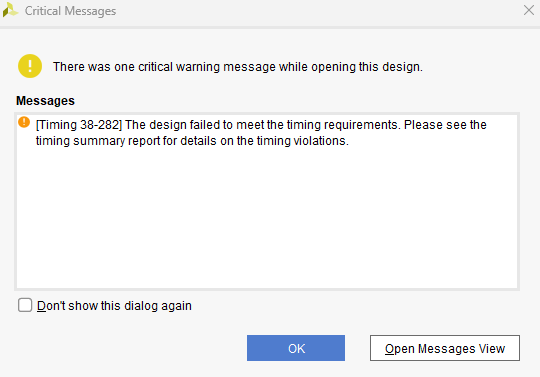
\includegraphics[width=\textwidth]{solutions/operation_chaining/3ns/critical.png}
    \caption{Vivado Operation Chaining Solution clk=3ns Timing Constraint Violated}
        \label{fig:left}
    \end{minipage}
    \hfill
    \begin{minipage}[t]{0.45\textwidth}
        \centering
        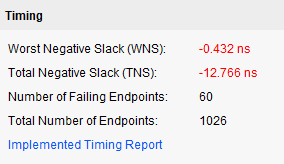
\includegraphics[width=\textwidth]{solutions/operation_chaining/3ns/wns.png}
    \caption{Vivado Operation Chaining Solution clk=3ns Timing Constraint Violated}
        \label{fig:right}
    \end{minipage}
\end{figure}

Pertanto, si procede con l'analisi dei report delle soluzioni hardware implementate in Vivado aventi periodo di clock coompreso nell'intervallo $[10ns,4ns]$.

\begin{table}[H]
    \centering
    \begin{tabular}{|c|c|c|c|c|c|c|c|}
        \hline
        \textbf{Solution} & \textbf{LUT} & \textbf{LUTRAM} & \textbf{FF} & \textbf{BRAM} & \textbf{DSP} & \textbf{IO} & \textbf{BUFG} \\
        \hline
        clk=10ns & 275 & 32 & 160 & 0 & 2 & 71 & 1 \\
        \hline
        clk=9ns & 276 & 32 & 226 & 0 & 2 & 71 & 1 \\
        \hline
        clk=8ns & 276 & 32 & 226 & 0 & 2 & 71 & 1 \\
        \hline
        clk=7ns & 186 & 32 & 222 & 0 & 4 & 71 & 1 \\
        \hline
        clk=6ns & 186 & 32 & 241 & 0 & 4 & 71 & 1 \\
        \hline
        clk=5ns & 186 & 32 & 258 & 0 & 4 & 71 & 1 \\
        \hline
        clk=4ns & 188 & 32 & 376 & 0 & 4 & 71 & 1 \\
        \hline
    \end{tabular}
    \caption{Vivado Operation Chaining Solution Utilization Report [\#]}
    \label{tab:vivado-operation-chaining-utilization-report}
\end{table}

\begin{figure}[H]
    \centering
    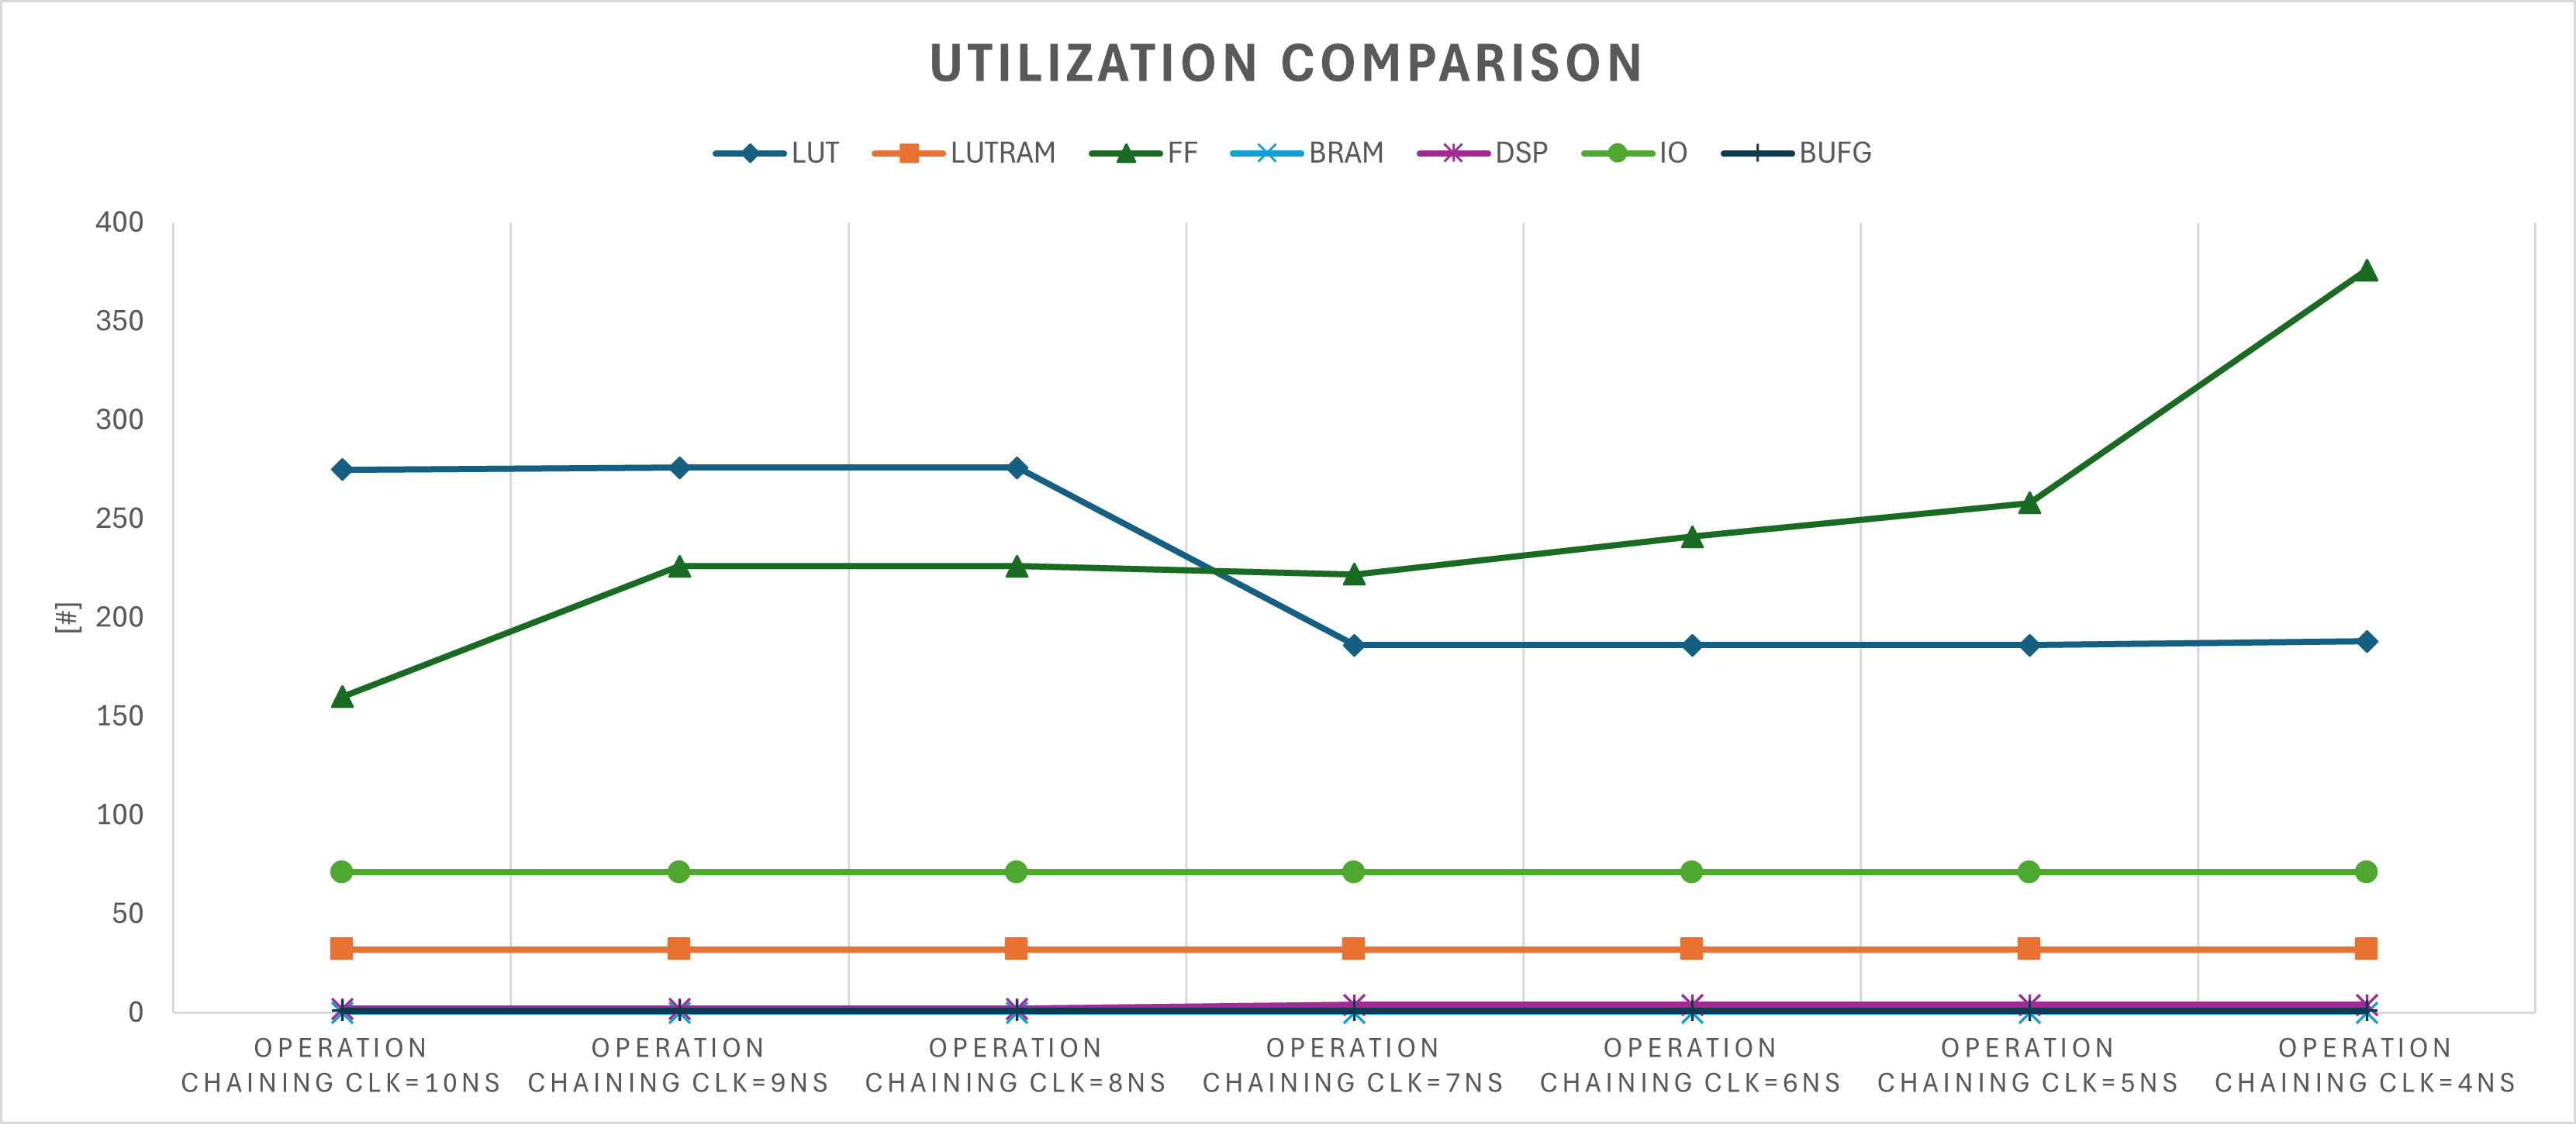
\includegraphics[width=\textwidth]{solutions/operation_chaining/operationchainingutilization.png}
    \caption{Vivado Operation Chaining Utilization Plot}
    \label{fig:vivado-operation-chaining-utilization-plot}
\end{figure}

\begin{table}[H]
    \centering
    \begin{tabular}{|c|c|c|c|c|}
        \hline
        \textbf{Solution} & \textbf{Cycles} [\#] & \textbf{Clock Constraint} [ns] & \textbf{WNS} [ns] & \textbf{Maximum Clock Frequency} [Mhz] \\
        \hline
        clk=10ns & 44 & 10 & 3.654 & 157.5795777 \\
        \hline
        clk=9ns & 55 & 9 & 3.06 & 168.3501684 \\
        \hline
        clk=8ns & 55 & 8 & 2.277 & 174.7335314 \\
        \hline
        clk=7ns & 66 & 7 & 1.33 & 176.366843 \\
        \hline
        clk=6ns & 88 & 6 & 1.573 & 225.8866049 \\
        \hline
        clk=5ns & 88 & 5 & 0.374 & 216.1694769 \\
        \hline
        clk=4ns & 131 & 4 & 0.454 & 282.0078962 \\
        \hline
    \end{tabular}
    \caption{Vivado Operation Chaining Solution Timing Report}
    \label{tab:vivado-operation-chaining-solution-timing-report}
\end{table}

\begin{figure}[H]
    \centering
    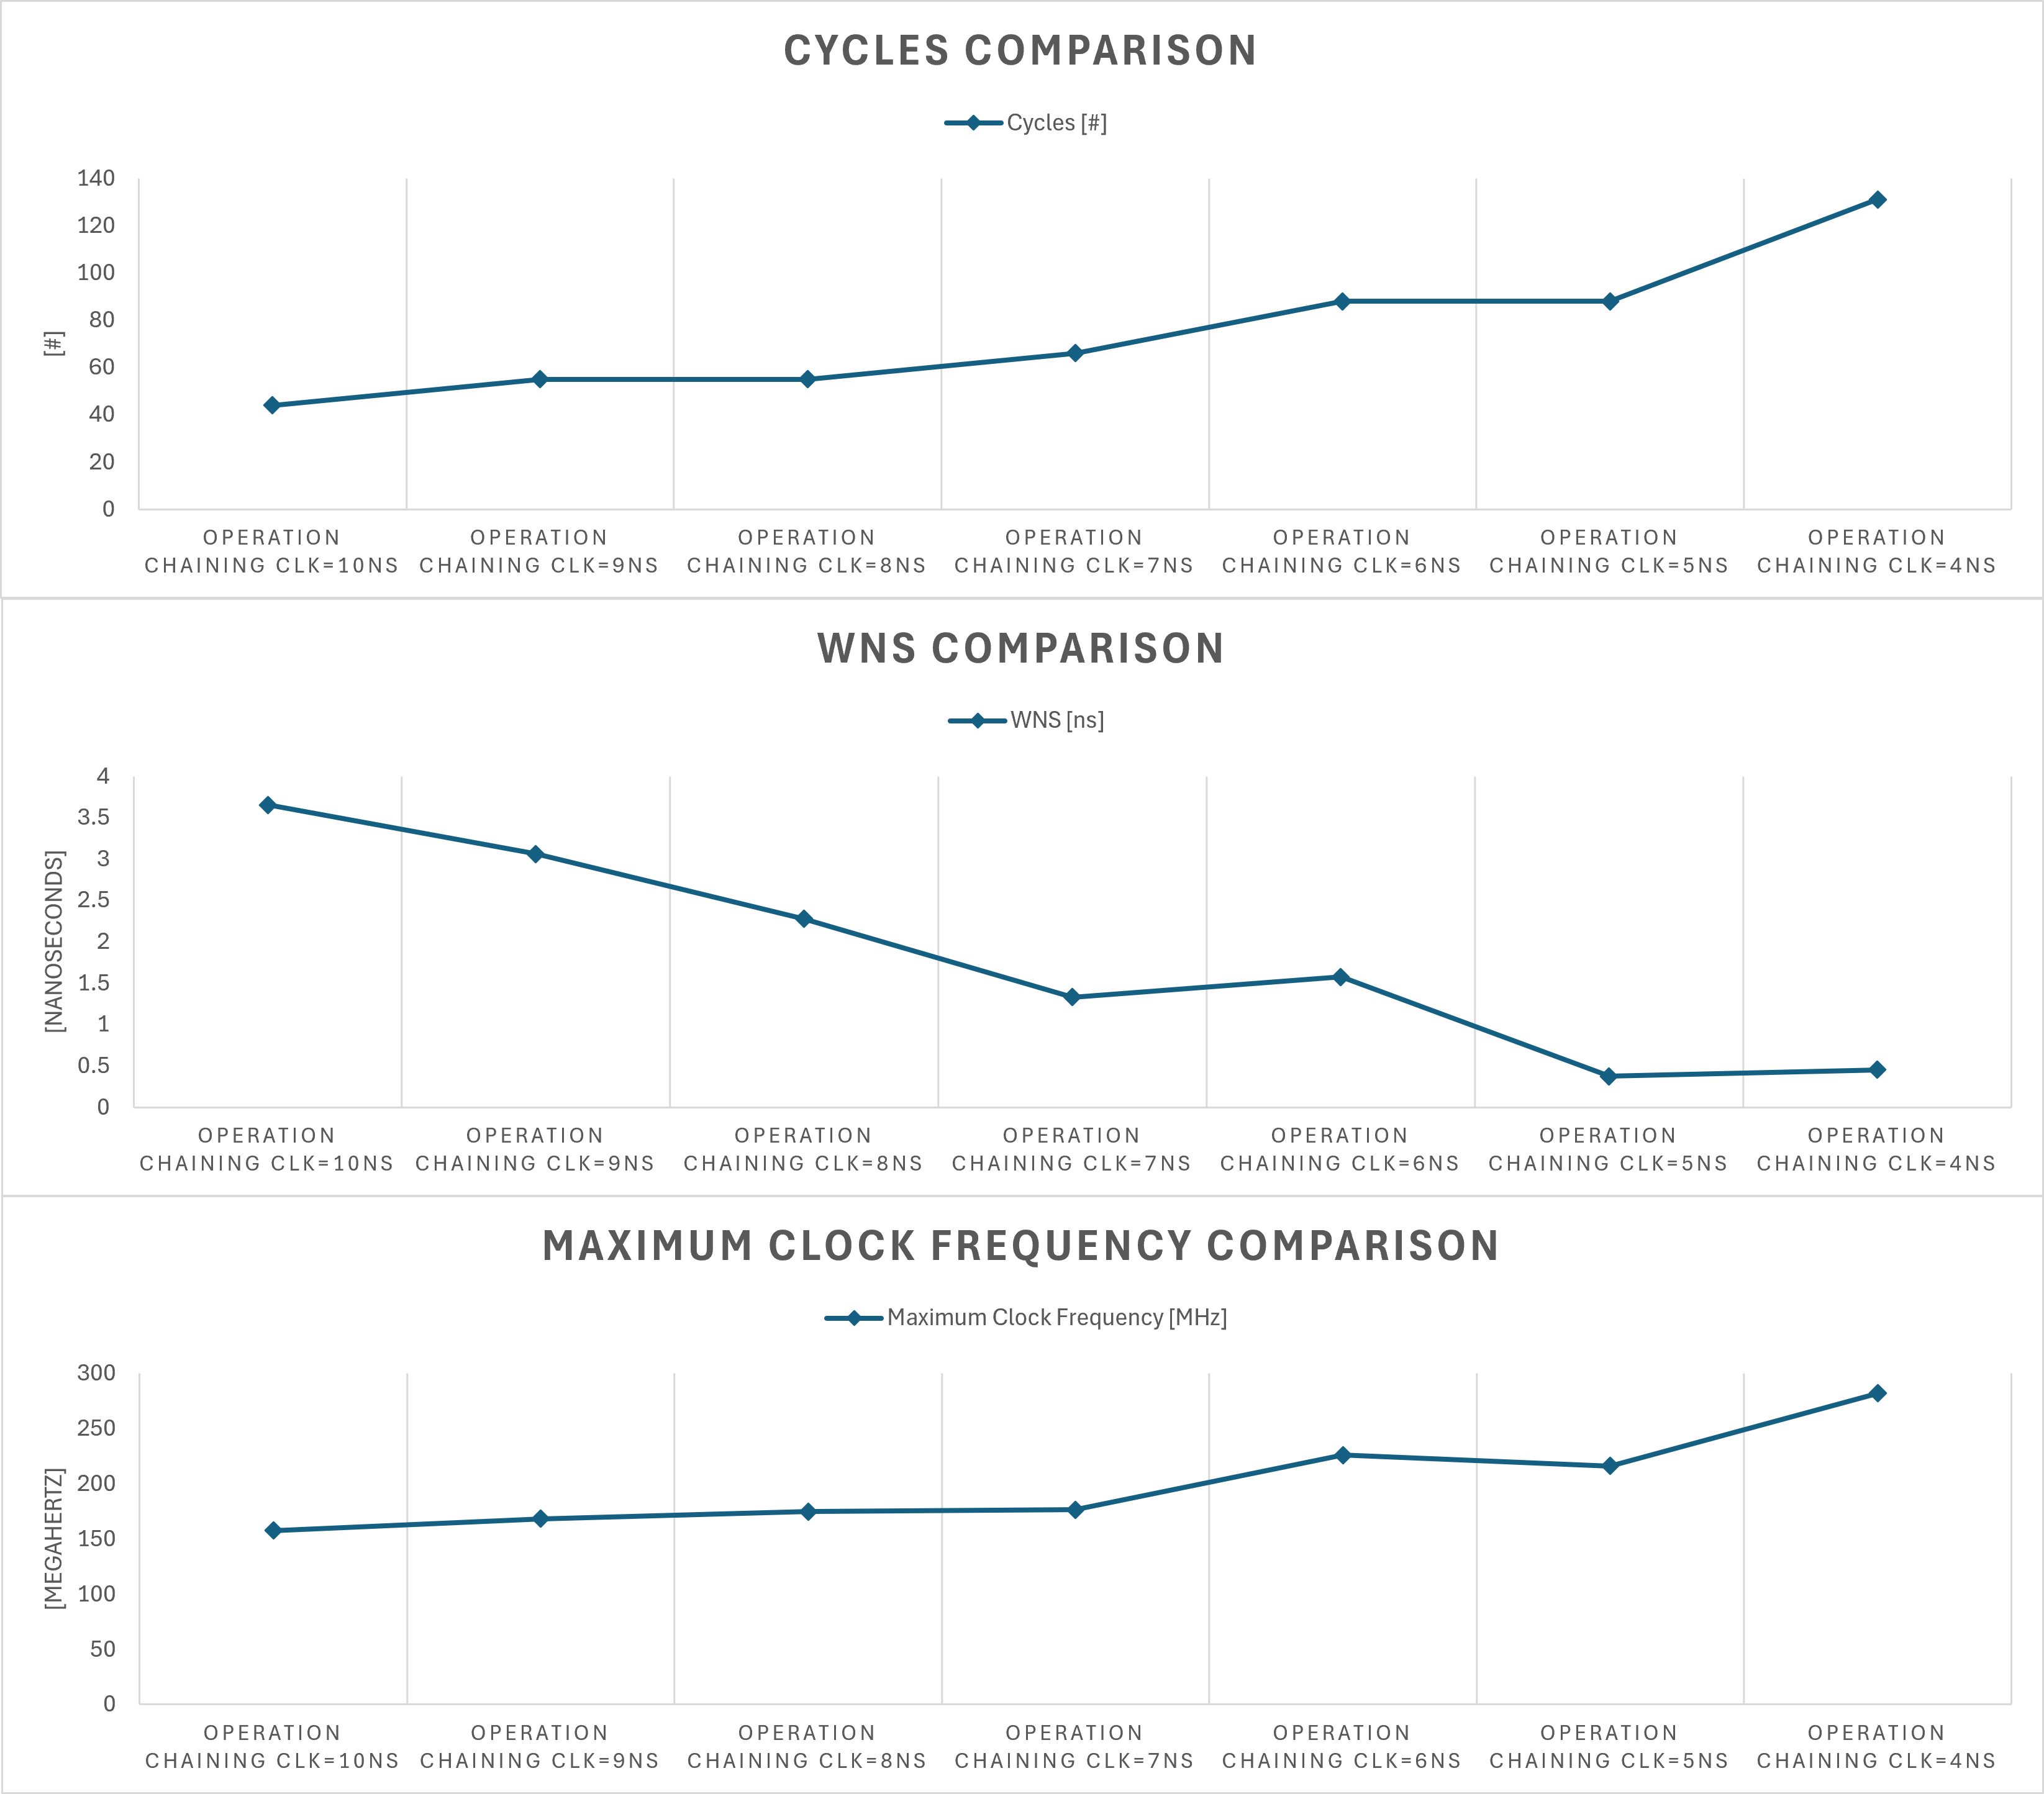
\includegraphics[width=\textwidth]{solutions/operation_chaining/operationchainingtiming.png}
    \caption{Vivado Operation Chaining Timing Plot}
    \label{fig:vivado-operation-chaining-timing-plot}
\end{figure}

Si può notare come in corrispondenza dell'architettura hardware a cui corrisponde un periodo di clock pari a 7ns si ha l'utilizzazione delle risorse minore a meno del numero di LUT e FF che risulta essere aumentato rispettivamente di un'unità e di 66 unità. Questo aumento di risorse può essere giustificato dal momento che, rispetto alla soluzione iniziale non ottimizzata a 10ns, il periodo del clock risulta essere diminuito e, pertanto, il tool prevede una gestione delle istruzioni in maniera più complessa comportando un'aumento delleee risorse stesse. Tanto è vero che al diminuire del periodo di clock, si ha un aumento delle risorse utilizzate e dei cicli di clock considerati per ottenere un nuovo risultato. In particolare, per quanto riguarda la massima frequenza di clock associata ad ogni soluzione proposta in questa sezione, si può notare come quella a cui corrisponde un periodo di clock pari a 7ns, presenta una maximum clock frequency maggiore rispetto a quelle avente periodo maggiore. Questo aumento lo si può, inoltre, evidenziare nelle successive soluzioni aventi periodo di clock ancora minore. Tanto è vero che il WNS, al diminuire del clock constraint, anch'esso diminuisce.

\begin{table}[H]
    \centering
    \begin{tabular}{|c|c|c|c|c|c|c|}
        \hline
        \textbf{Solution} & \textbf{Clock Enable} & \textbf{Clocks} & \textbf{DSP} & \textbf{Logic} & \textbf{Set/Reset} & \textbf{Data} \\
        \hline
        clk=10ns & 0.455035944 & 1.215706812 & 0.343570428 & 0.925468281 & 0.00349783 & 1.014495501 \\
        \hline
        clk=9ns & 0.371109403 & 1.601127908 & 0.308091694 & 0.871003722 & 0.003504661 & 0.845550094 \\
        \hline
        clk=8ns & 0.432465255 & 1.790320966 & 0.364705513 & 1.03614782 & 0.003386509 & 1.085355412 \\
        \hline
        clk=7ns & 0.4179838 & 1.991891069 & 0.305155962 & 0.881534419 & 0.002575182 & 0.757947506 \\
        \hline
        clk=6ns & 0.367850007 & 2.092533279 & 0.244985771 & 0.788475969 & 0.00273619 & 0.666663051 \\
        \hline
        clk=5ns & 0.556948828 & 3.174162703 & 0.291668839 & 0.943421735 & 0.004532358 & 0.906153 \\
        \hline
        clk=4ns & 0.57213963 & 3.804846667 & 0.253423554 & 0.799402245 & 0.002476984 & 0.756326073 \\
        \hline
    \end{tabular}
    \caption{Vivado Operation Chaining Solution Dynamic Power Report [mW]}
    \label{tab:vivado-operation-chaining-solution-dynamic-power-reproot}
\end{table}

\begin{table}[H]
    \centering
    \begin{minipage}[t]{0.45\linewidth}
        \centering
        \begin{tabular}{|c|c|}
            \hline
            \textbf{Solution} & \textbf{Dynamic Total} \\
            \hline
            clk=10ns & 3.957774796 \\
            \hline
            clk=9ns & 4.000387481 \\
            \hline
            clk=8ns & 4.712381475 \\
            \hline
            clk=7ns & 4.357087937 \\
            \hline
            clk=6ns & 4.163244267 \\
            \hline
            clk=5ns & 5.876887463 \\
            \hline
            clk=4ns & 6.188615153 \\
            \hline
        \end{tabular}
        \caption{Vivado Operation Chaining Solution Dynamic Power Report [mW]}
        \label{tab:vivado-operation-chaining-solution-dynamic-power-reproot}
    \end{minipage}
    \hfill
    \centering
    \begin{minipage}[t]{0.45\linewidth}
        \centering
        \begin{tabular}{|c|c|}
            \hline
            \textbf{Solution} & \textbf{Energy Single Operation} \\
            \hline
            clk=10ns & 39.57774796 \\
            \hline
            clk=9ns & 36.00348733 \\
            \hline
            clk=8ns & 37.6990518 \\
            \hline
            clk=7ns & 30.49961556 \\
            \hline
            clk=6ns & 24.9794656 \\
            \hline
            clk=5ns & 29.38443731 \\
            \hline
            clk=4ns & 24.75446061 \\
            \hline
        \end{tabular}
        \caption{Vivado Operation Chaining Solution Energy Single Operation Report [pJ]}
        \label{tab:vivado-operation-chaining-solution-solution-energy-single-operation-reproot}
    \end{minipage}
\end{table}

\begin{figure}[H]
    \centering
    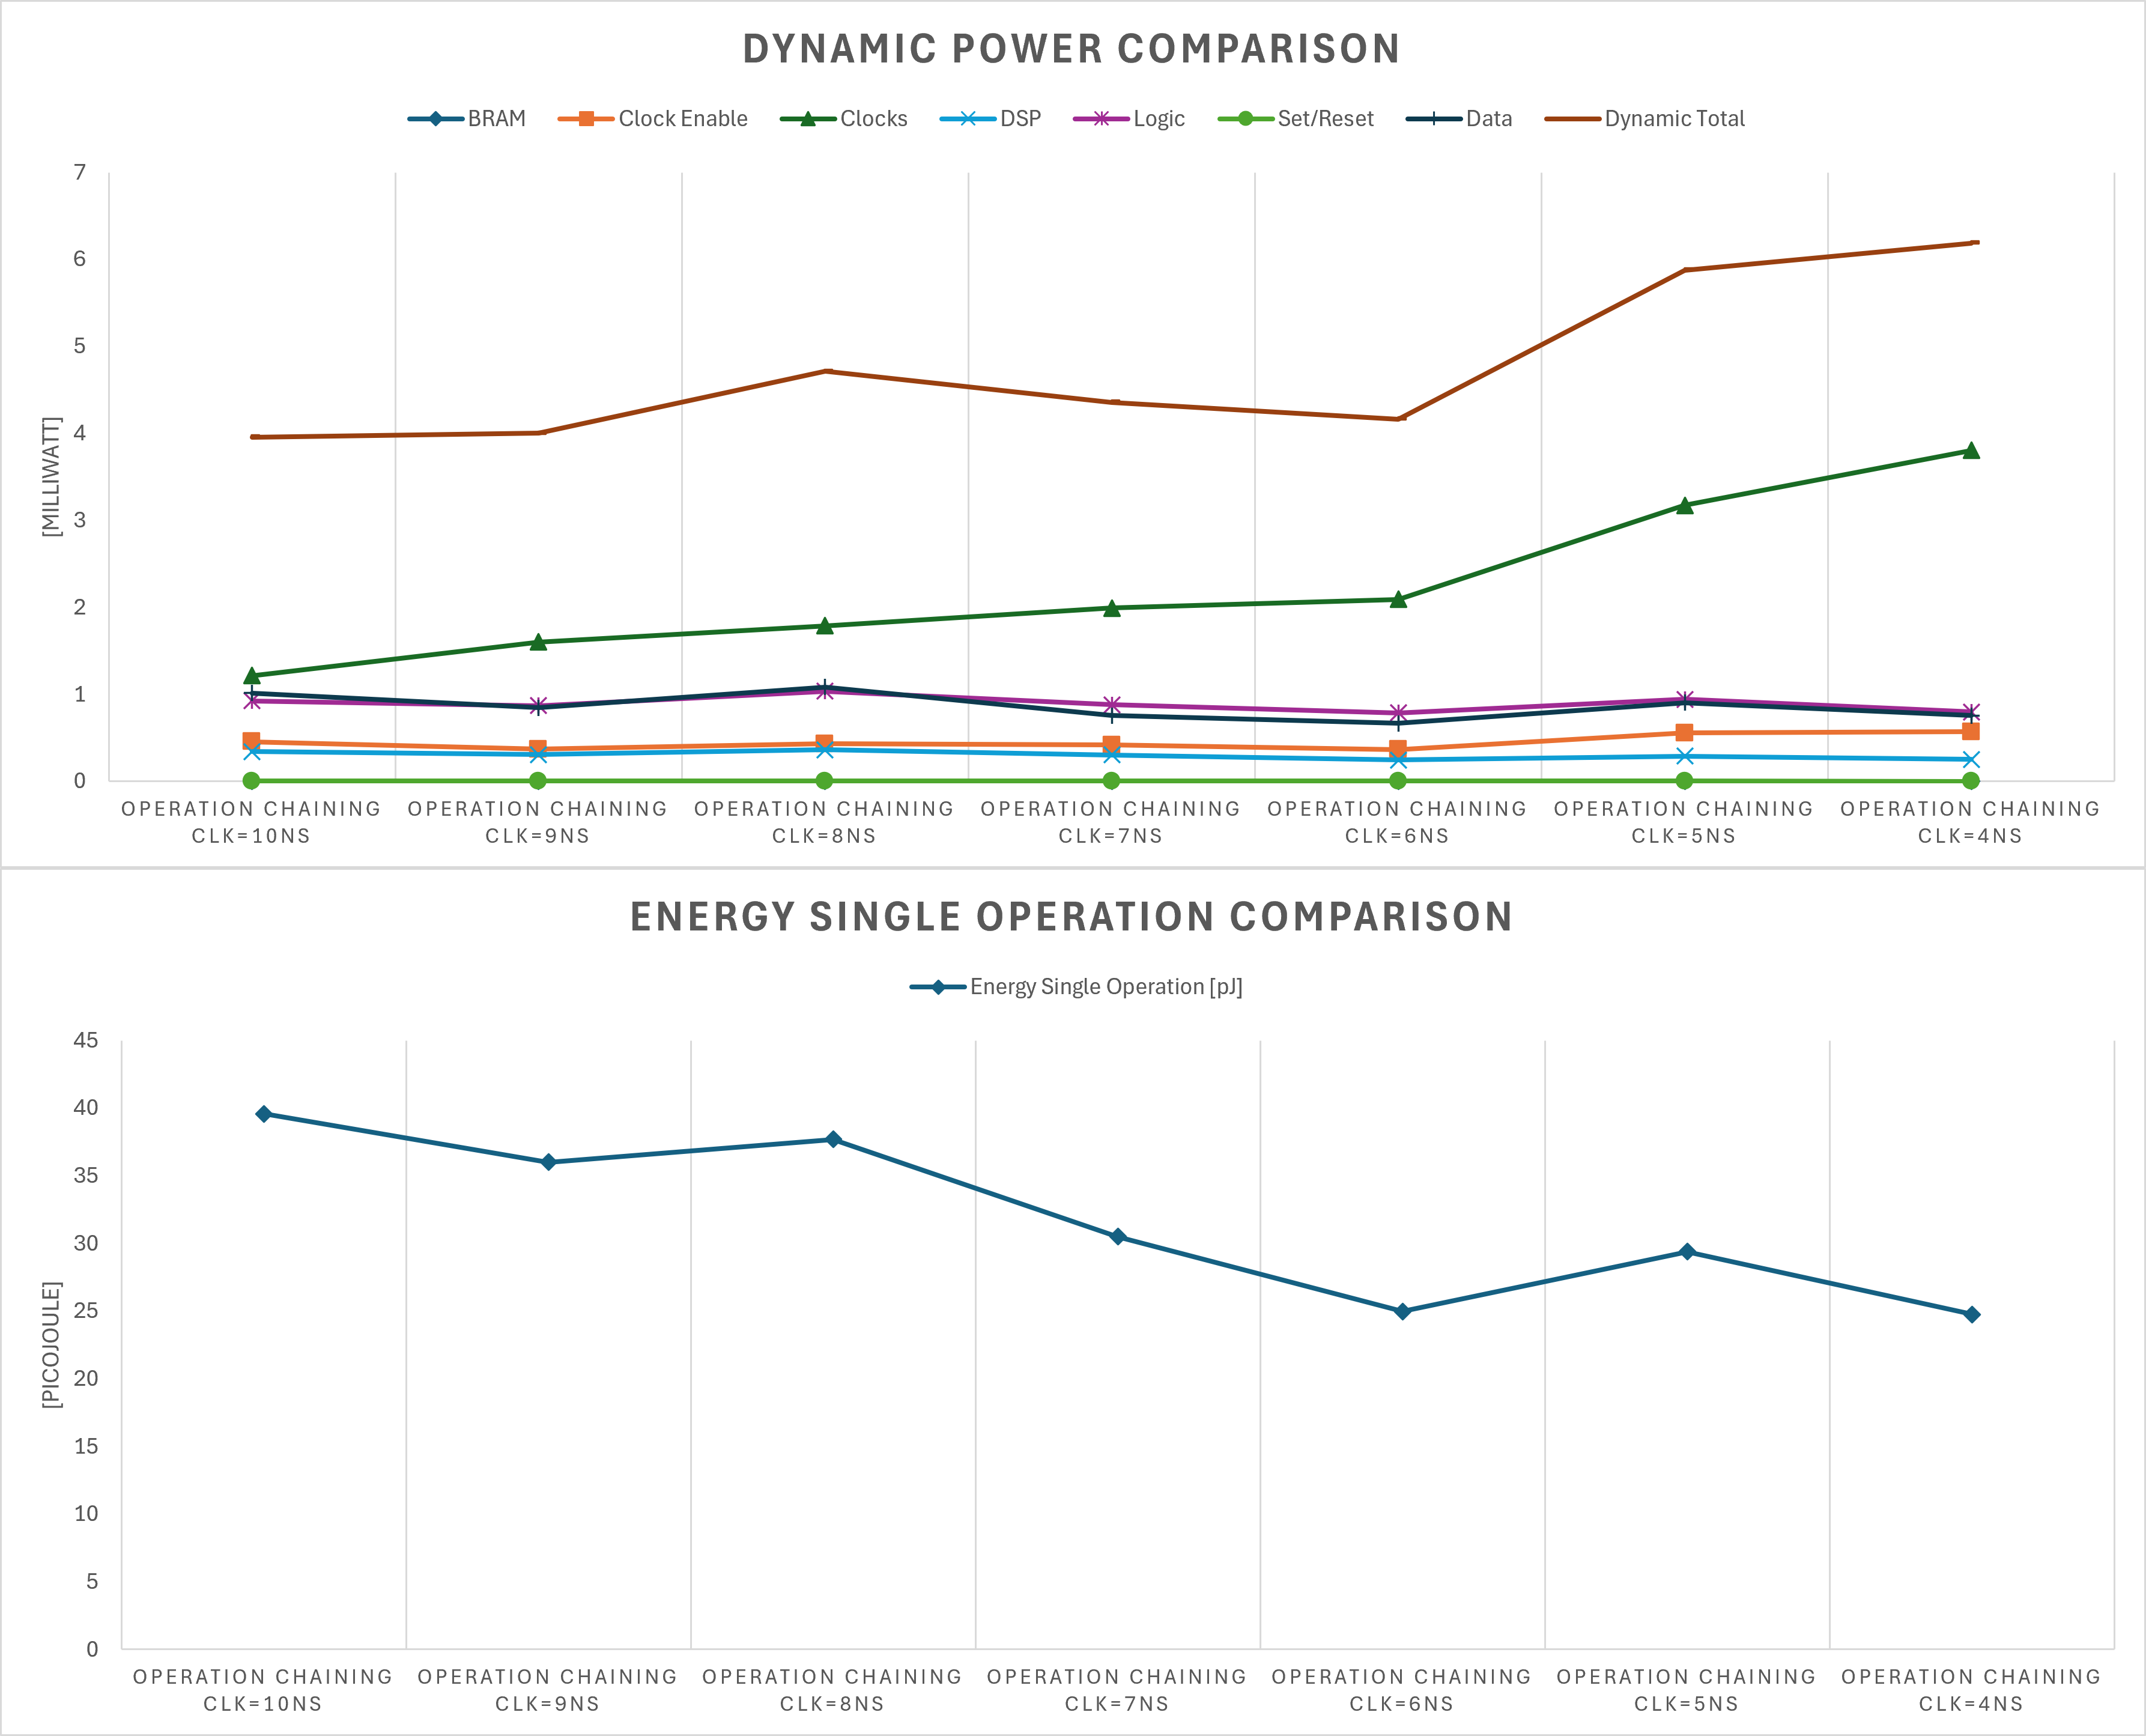
\includegraphics[width=\textwidth]{solutions/operation_chaining/operationchainingpower.png}
    \caption{Vivado Operation Chaining Power Plot}
    \label{fig:vivado-operation-chaining-power-plot}
\end{figure}

Si può notare come la potenza dinamica aumenti al diminuire del periodo di clock considerato. Questo si evince dal fatto che l'utilizzazione delle risorse (in particolar modo per quello che riguarda i FF) aumenta al diminuire del constraint di clock. Tanto è vero che la potenza dinamica associata all'albero di distribuzione del clock (BUFG) e del clock enable sia di gran lunga maggiore rispetto alla soluzione iniziale dove è stato considerato un constraint pari a 10ns. In particolare, questo aumento di potenza dinamica può essere associato al maggior numero di Flip Flop utilizzato nelle soluzioni aventi periodo di clock sempre minore.
\\
Pertanto, considerando i report di utilizzazione delle risorse, di timing, di potenza dinamica ed energia per singola operazione, si può evincere che la soluzione hardware che permette un trade-off ottimale è quella ottenuta in corrispondenza del periodo di clock pari a 7ns.
\newpage

\subsection{Code Hoisting Solution}
Considerando, ora, la stessa architettura software precedentemente utilizzata, si potrebbe mettere il luce un possibile problema: impiego di risorse aggiuntive a causa di istruzioni logiche condizionali. In particolare, questo problema è dovuto al fatto che, all'interno del ciclo for, è prevista l'istruzione condizionale $if(i == 0)$ che comporta l'utilizzo di risorse hardware addizionali. Bisogna precisare che, istruzioni logiche quali $if$, $else$ e $then$ rendono i loop inefficienti limitando le performance dal punto di vista hardware.
Fondamentalmente, l'istruzione condizionale $if(i == 0)$ a livello hardware si traduce nel leggere il valore dell'indice $i$ in una certa struttura dati ed effettuare il confronto, tramite un comparatore, tra tale valore appena citato e il valore zero.

\lstinputlisting[language=C++]{solutions/code_hoisting/fir_code_hoisting.cpp}

Pertanto, si potrebbe pensare di eliminare l'$if$ in questione e spostarlo al di fuori del loop. In questo modo, anche l'istruzione condizionale $else$, che ricopriva il resto delle iterazioni, verrà gestita direttamente all'interno del loop avente quest'ultimo un'iterazione in meno dovuto ai motivi appena citati. Pertanto, quello che ci si aspetta è una diminuzione dal punto di vista della latenza totale, dal punto di vista delle risorse e per ciò che riguarda la potenza dinamica associata alla parte di logica dell'architettura hardware in questione. 
\\
Pertanto, si mostrano qui di seguito i report, generati da HLS, riguardo la sintesi, la C/RTL Cosimulation e l'Export RTL.

\begin{table}[H]
    \centering
    \begin{minipage}[t]{0.45\linewidth}
        \centering
        \begin{tabular}{|c|c|c|c|}
            \hline
            \textbf{Clock} & \textbf{Target} & \textbf{Estimated} & \textbf{Uncertainty} \\
            \hline
            ap\_clk & 10.00 & 8.510 & 1.25 \\
            \hline
        \end{tabular}
        \caption{HLS Code Hoisting Solution Timing Summary (ns)}
        \label{tab:hls-code-hoisting-solution-timing-summary}
    \end{minipage}
    \hfill
    \begin{minipage}[t]{0.45\linewidth}
        \centering
        \begin{tabular}{|c|c|c|c|}
            \hline
            \multicolumn{2}{|c|}{\textbf{Latency}} & \multicolumn{2}{|c|}{\textbf{Interval}} \\
            min & max & min & max \\
            \hline
            42 & 42 & 42 & 42 \\
            \hline
        \end{tabular}
        \caption{HLS Code Hoisting Solution Latency Summary (clock cycles)}
        \label{tab:hls-code-hoisting-solution-latency-summary}
    \end{minipage}
\end{table}

\begin{table}[H]
    \centering
    \begin{tabular}{|c|c|c|c|c|c|c|c|}
        \hline
        \multicolumn{1}{|c|}{Loop} & \multicolumn{2}{|c|}{\textbf{Latency}} & \multicolumn{1}{c|}{\textbf{Iteration Latency}} & \multicolumn{2}{c|}{\textbf{Initiation Interval}} & \multicolumn{1}{c|}{\textbf{Trip Count}}  \\
        Name & min & max & & achieved & target &  \\
        \hline
        - loop & 40 & 40 & 4 & - & - & 10 \\
        \hline
    \end{tabular}
    \caption{HLS Code Hoisting Solution Latency Loops Summary }
    \label{tab:hls-code-hoisting-solution-loop-summary}
\end{table}

Si può notare come il numero di iterazioni del loop, in questo caso, sia pari a 10 tale che la latenza totale del ciclo risulta essere pari a 40.

\begin{figure}[H]
    \centering
    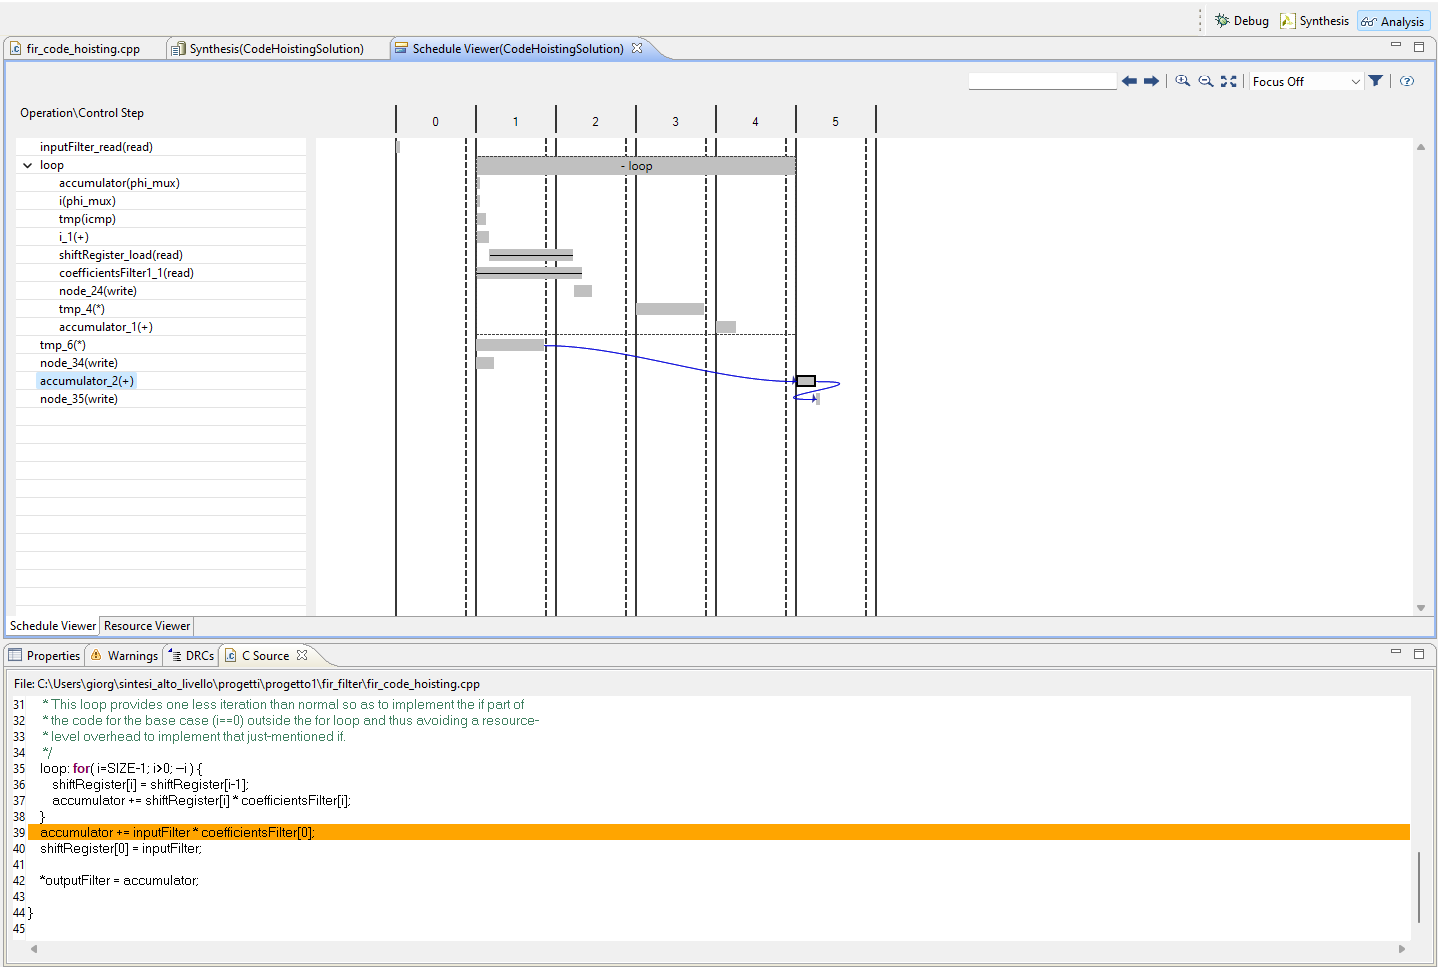
\includegraphics[width=1\textwidth]{solutions/code_hoisting/codehoistinganalysis.png}
    \caption{HLS Code Hoisting Solution Trip Count Analysis}
\end{figure}

In particolare, è opportuno fare un'attenta riflessione riguardo la latenza totale dell'architettura hardware in questione. Il report di sintesi, effettivamente, ha restituito una stima di tale valore pari a 42 dal momento bisogna considera una latenza totale del loop pari a 40, un ciclo di latency ulteriore dovuto alla lettura iniziale dell'input (come avviene per ogni soluzione progettata) e, come ultimo, un altro ciclo finale dovuto alle due operazioni in parallelo effettuate: accumulo associato al coefficiente in posizione 0 e scrittura del dato in uscita. Precedentemente, nella soluzione iniziale non ottimizzata, tale latenza finale non era prevista dal momento che il caso $i==0$ veniva gestito all'interno del loop mediante istruzione condizionale e la scrittura del dato in uscita veniva effettuata in parallelo all'operazione appena citata.

\begin{table}[h]
    \centering
    \begin{tabular}{|l|c|c|c|c|}
        \hline
        \textbf{Name}    & \textbf{BRAM\_18K} & \textbf{DSP48E} & \textbf{FF} & \textbf{LUT} \\ \hline
        DSP              & -                   & -               & -           & -            \\ 
        Expression       & -                   & 4               & 0           & 140          \\ 
        FIFO             & -                   & -               & -           & -            \\ 
        Instance         & -                   & -               & -           & -            \\ 
        Memory           & 0                   & -               & 74          & 8            \\ 
        Multiplexer      & -                   & -               & -           & 92          \\ 
        Register         & -                   & -               & 156         & -            \\ \hline
        \textbf{Total}   & 0                   & 4               & 230         & 240          \\ \hline
        \textbf{Available} & 280               & 220             & 106400      & 53200        \\ \hline
        \textbf{Utilization (\%)} & 0            & 1               & $\sim$0     & $\sim$0      \\ \hline
    \end{tabular}
    \caption{HLS Code Hoisting Solution Utilization Estimates Summary}
    \label{tab:hls-code-hoisting-solution-utilization-estimates-summary}
\end{table}

Si può notare come il report di C/RTL Cosimulation evidenzi un ciclo di latenza in meno rispetto alla soluzione hardware iniziale non ottimizzata. Questo è dovuto al fatto che, come precedentemente citato, il loop presenta un'iterazione in meno tale per cui il numero di cicli di clock, affinché venga processato si abbia un risultato in uscita, è pari a 43 rispetto ai 44 corrispondenti alla soluzione non ottimizzata.

\begin{table}[H]
    \centering
    \begin{tabular}{|c|c|c|c|c|c|c|c|}
        \hline
        \multicolumn{1}{|c|}{RTL} & \multicolumn{1}{|c|}{Status} & \multicolumn{3}{c|}{\textbf{Latency}} & \multicolumn{3}{c|}{\textbf{Interval}} \\
        &  & min & avg & max & min & avg & max \\
        \hline
        VHDL & Pass & 42 & 42 & 43 & 42 & 42 & 43 \\
        \hline
    \end{tabular}
    \caption{HLS Code Hoisting Solution C/RTL Cosimulation Summary }
    \label{tab:hls-code-hoisting-solution-cosimulation-summary}
\end{table}

Inoltre, si può notare come il numero di risorse relative alla soluzione hardware in questione risulta essere pressocché il medesimo tranne per il numero di FF che risulta essere ridotto di circa il 18\%.

\begin{table}[H]
    \centering
    \begin{minipage}[t]{0.45\linewidth}
        \centering
        \begin{tabular}{|l|r|}
            \hline
            \textbf{Resource} & \textbf{VHDL} \\
            \hline
            SLICE & 75 \\
            \hline
            LUT & 270 \\
            \hline
            FF & 131 \\
            \hline
            DSP & 2 \\
            \hline
            BRAM & 0 \\
            \hline
            SRL & 0 \\
            \hline
        \end{tabular}
        \caption{HLS Code Hoisting Solution Export RTL Resource Usage}
        \label{tab:hls-code-hoisting-solution-export-rtl-resoruce-usage}
    \end{minipage}
    \hfill
    \begin{minipage}[t]{0.45\linewidth}
        \centering
        \begin{tabular}{|l|r|}
            \hline
            \textbf{Timing} & \textbf{VHDL} \\
            \hline
            CP required & 10.000 \\
            \hline
            CP achieved post-synthesis & 5.745 \\
            \hline
            CP achieved post-implementation & 6.847 \\
            \hline
        \end{tabular}
        \caption{HLS Code Hoisting Solution Export RTL Final Timing}
        \label{tab:hls-code-hoisting-solution-export-rtl-final-timing}
    \end{minipage}
\end{table}

Pertanto, importando l'IP in Vivado e impostando un clock constraint pari a 10ns è possibile analizzare i seguenti report di risorse, timing, potenza dinamica ed energia per singola operazione.
\lstinputlisting[language=VHDL]{solutions/code_hoisting/clk_constraint.xdc}

\begin{table}[H]
    \centering
    \begin{tabular}{|c|c|c|c|c|c|c|}
        \hline
        \textbf{LUT} & \textbf{LUTRAM} & \textbf{FF} & \textbf{BRAM} & \textbf{DSP} & \textbf{IO} & \textbf{BUFG} \\
        \hline
        270 & 32 & 134 & 0 & 2 & 71 & 1 \\
        \hline
    \end{tabular}
    \caption{Vivado Code Hoisting Solution Utilization Report [\#]}
    \label{tab:vivado-code-hoisting-solution-utilization-reproot}
\end{table}

Dal momento che il WNS è diminuito, si può notare come la maximum clock frequency sia diminuita rispetto alla soluzione non ottimizzata.

\begin{table}[H]
    \centering
    \begin{tabular}{|c|c|c|c|}
        \hline
        \textbf{Cycles} [\#] & \textbf{Clock Constraint} [ns] & \textbf{WNS} [ns] & \textbf{Maximum Clock Frequency} [Mhz] \\
        \hline
        43 & 10 & 3.074 & 144.3834825 \\
        \hline
    \end{tabular}
    \caption{Vivado Code Hoisting Solution Timing Report}
    \label{tab:vivado-code-hoisting-solution-timing-reproot}
\end{table}

Per quanto riguarda la potenza dinamica e l'energia per singola operazione, si evidenzia un aumento rispetto alla soluzione iniziale. Si può ipotizzare che, dal punto di vista della potenza, il tool riesca meglio ad ottimizzare direttamente tutte le operazioni relative ad accumulo e shifting nello stesso ciclo, anziché avere 10 operazioni all'interno del loop e una fuori dal ciclo. 
\begin{table}[H]
    \centering
    \begin{tabular}{|c|c|c|c|c|c|c|}
        \hline
        \textbf{BRAM} & \textbf{Clock Enable} & \textbf{Clocks} & \textbf{DSP} & \textbf{Logic} & \textbf{Set/Reset} [mW] & \textbf{Data} \\
        \hline
        0 & 0.370487687 & 1.756788697 & 0.41467679 & 0.838255044 & 3.35E-03 & 1.381990616 \\
        \hline
    \end{tabular}
    \caption{Vivado Code Hoisting Solution Dynamic Power Report [mW]}
    \label{tab:vivado-code-hoisting-solution-dynamic-power-reproot}
\end{table}

\begin{table}[H]
    \centering
    \begin{minipage}[t]{0.45\linewidth}
        \centering
        \begin{tabular}{|c|}
            \hline
            \textbf{Dynamic Total} \\
            \hline
            4.765546238 \\
            \hline
        \end{tabular}
        \caption{Vivado Code Hoisting Solution Dynamic Power Report [mW]}
        \label{tab:vivado-code-hoisting-solution-dynamic-power-reproot}
    \end{minipage}
    \hfill
    \centering
    \begin{minipage}[t]{0.45\linewidth}
        \centering
        \begin{tabular}{|c|}
            \hline
            \textbf{Energy Single Operation} \\
            \hline
            47.65546238 \\
            \hline
        \end{tabular}
        \caption{Vivado Code Hoisting Solution Energy Single Operation Report [pJ]}
        \label{tab:vivado-code-hoisting-solution-energy-single-operation-reproot}
    \end{minipage}
\end{table}

Pertanto, se da una parte si è ottenuto una piccola diminuzione delle risorse avendo gestito l'overhead di risorse dovuto alle istruzioni condizionali presenti all'interno del loop, dall'altra parte si è ottenuto un aumento di circa il 21\% della potenza dinamica rispetto alla soluzione iniziale non ottimizzata.
\newpage

\subsection{Loop Fission Solution}
Considerando la soluzione precedente, si è risolto la possibile problematica di overhead delle risorse dovuta alle istruzioni condizionali presenti all'interno del loop. Bisogna notare, però, che all'interno di tale ciclo for siano presenti istruzioni potenzialmente complesse dal punto di vista computazionale. In particolare, il tool, durante la compilazione del codice, cerca in qualche modo di apportare qualche tipologia di ottimizzazione al loop in questione. Pertanto, si potrebbe pensare di implementare due loop: uno per l'operazione di shifting ed un altro per l'operazione di accumulo. Quindi, effettuando la scissione del loop, relativo alla soluzione precedente, si potrebbe pensare che il tool possa effettuare tali ottimizzazioni in maniera più efficiente dal momento che le ottimizzazioni verrebbero effettuate su due cicli distinti. Quello che ci si aspetta, però, è un aumento significativo della latenza totale dovuto al fatto che, in questo caso, bisogna considerare la latenza di due loop.
\lstinputlisting[language=C++]{solutions/loop_fission/fir_loop_fission.cpp}

Effettuando la sintesi, la C/RTL Cosimulation ed Export RTL si ottengono i seguenti report.

\begin{table}[H]
    \centering
    \begin{minipage}[t]{0.45\linewidth}
        \centering
        \begin{tabular}{|c|c|c|c|}
            \hline
            \textbf{Clock} & \textbf{Target} & \textbf{Estimated} & \textbf{Uncertainty} \\
            \hline
            ap\_clk & 10.00 & 8.510 & 1.25 \\
            \hline
        \end{tabular}
        \caption{HLS Loop Fission Solution Timing Summary (ns)}
        \label{tab:hls-loop-fission-solution-timing-summary}
    \end{minipage}
    \hfill
    \begin{minipage}[t]{0.45\linewidth}
        \centering
        \begin{tabular}{|c|c|c|c|}
            \hline
            \multicolumn{2}{|c|}{\textbf{Latency}} & \multicolumn{2}{|c|}{\textbf{Interval}} \\
            min & max & min & max \\
            \hline
            66 & 66 & 66 & 66 \\
            \hline
        \end{tabular}
        \caption{HLS Loop Fission Solution Latency Summary (clock cycles)}
        \label{tab:hls-loop-fission-solution-latency-summary}
    \end{minipage}
\end{table}

Si può notare come la latenza sia aumentata rispetto alle soluzioni precedenti in cui era presente un solo loop. Questo può essere, inoltre, analizzato nella tabella "Table 38: HLS Loop Fission Solution Latency Loops Summary" sotto allegata dove è possibile osservare che i due loop vengono riconosciuti come due loop indipendenti tra loro e con una latenza associata. In particolare, "loopShifting" presenta un trip count pari a 10 dal momento che il caso $i==0$ viene gestito secondo la tecnica del code hoisting, cioè al di fuori del ciclo stesso.

\begin{table}[H]
    \centering
    \begin{tabular}{|c|c|c|c|c|c|c|c|c|}
        \hline
        \multicolumn{1}{|c|}{Loop} & \multicolumn{2}{|c|}{\textbf{Latency}} & \multicolumn{2}{c|}{\textbf{Iteration Latency}} & \multicolumn{2}{c|}{\textbf{Initiation Interval}} & \multicolumn{1}{c|}{\textbf{Trip Count}}  \\
        Name & min & max & min & max & achieved & target &  \\
        \hline
        - loopShifting & 20 & 20 & 2 & 2 & - & - & 10 \\
        - loopAccumulator & 44 & 44 & 4 & 4 & - & - & 11 \\
        \hline
    \end{tabular}
    \caption{HLS Loop Fission Solution Latency Loops Summary }
    \label{tab:hls-loop-fission-solution-loop-summary}
\end{table}

\begin{figure}[H]
    \centering
    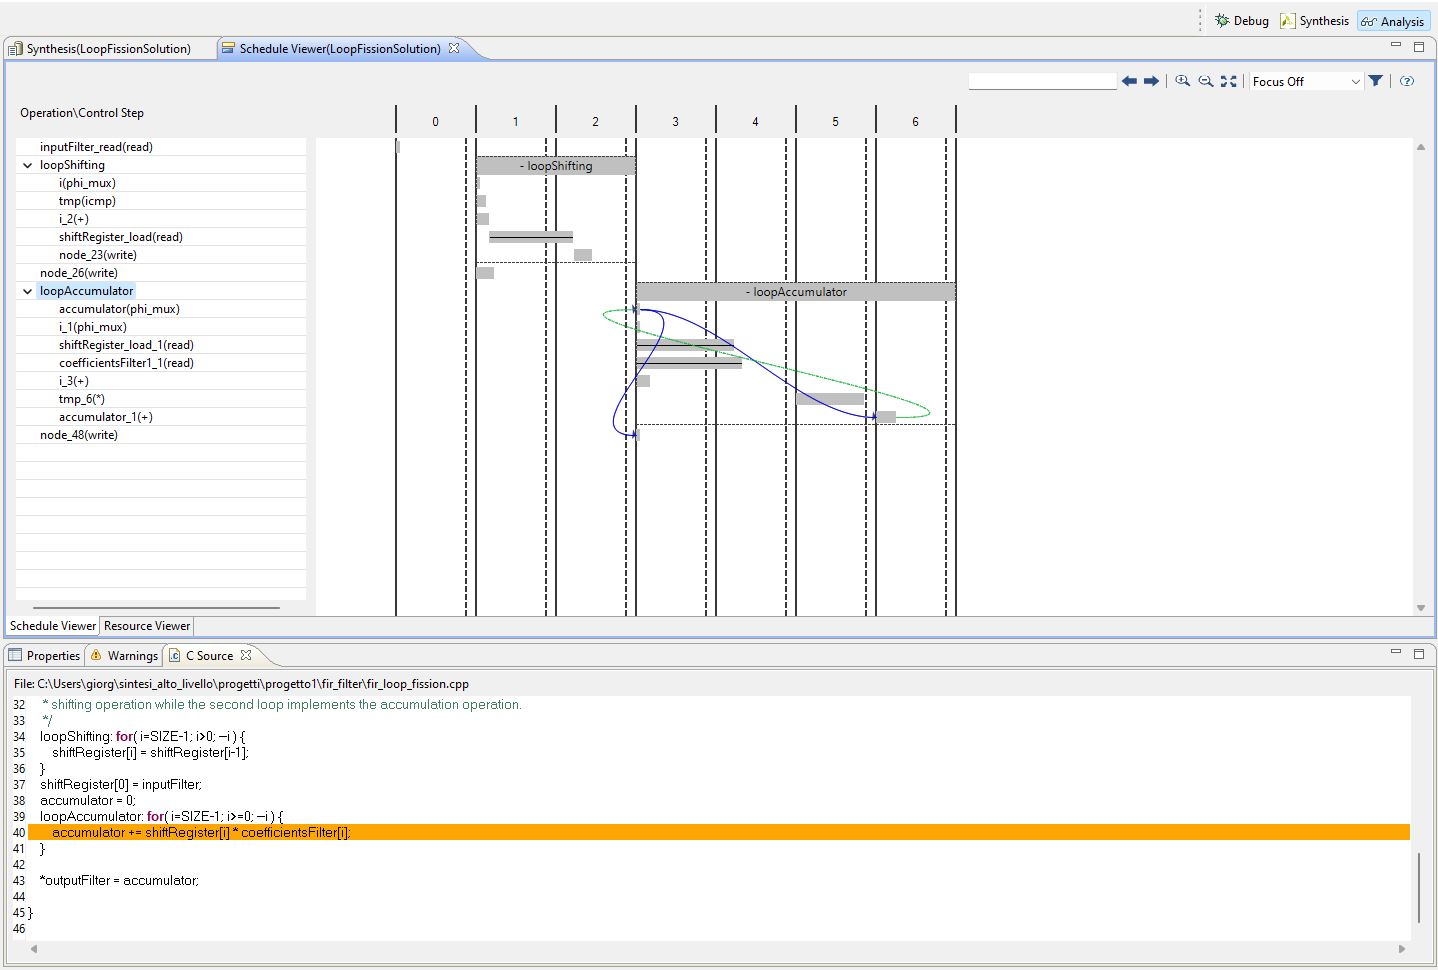
\includegraphics[width=1\textwidth]{solutions/loop_fission/loopfissionanalysis.png}
    \caption{HLS Loop Fission Solution Analysis}
\end{figure}

La scissione del loop nei cicli "loopShifting" e "loopAccumulator" la si può notare, inoltre, nella figura sopra allegata che mostra la finestra di \textit{Analysis}. Bisogna di nuovo precisare che, tale tecnica ha l'obiettivo di favorire il tool di ottimizzare i due loop in maniera indipendente effettuando magari uno scheduling delle operazioni differente, attraverso procedure proprietarie, rispetto alle soluzioni precedenti dove era previsto un ciclo for unico. 

\begin{table}[h]
    \centering
    \begin{tabular}{|l|c|c|c|c|}
        \hline
        \textbf{Name}    & \textbf{BRAM\_18K} & \textbf{DSP48E} & \textbf{FF} & \textbf{LUT} \\ \hline
        DSP              & -                   & -               & -           & -            \\ 
        Expression       & -                   & 2               & 0           & 96          \\ 
        FIFO             & -                   & -               & -           & -            \\ 
        Instance         & -                   & -               & -           & -            \\ 
        Memory           & 0                   & -               & 74          & 8            \\ 
        Multiplexer      & -                   & -               & -           & 110          \\ 
        Register         & -                   & -               & 131         & -            \\ \hline
        \textbf{Total}   & 0                   & 2               & 205         & 214          \\ \hline
        \textbf{Available} & 280               & 220             & 106400      & 53200        \\ \hline
        \textbf{Utilization (\%)} & 0            & $\sim$0               & $\sim$0     & $\sim$0      \\ \hline
    \end{tabular}
    \caption{HLS Loop Fission Solution Utilization Estimates Summary}
    \label{tab:hls-loop-fission-solution-utilization-estimates-summary}
\end{table}

\begin{table}[H]
    \centering
    \begin{tabular}{|c|c|c|c|c|c|c|c|}
        \hline
        \multicolumn{1}{|c|}{RTL} & \multicolumn{1}{|c|}{Status} & \multicolumn{3}{c|}{\textbf{Latency}} & \multicolumn{3}{c|}{\textbf{Interval}} \\
        &  & min & avg & max & min & avg & max \\
        \hline
        VHDL & Pass & 66 & 66 & 67 & 66 & 66 & 67 \\
        \hline
    \end{tabular}
    \caption{HLS Loop Fissiong Solution C/RTL Cosimulation Summary }
    \label{tab:hls-loop-fission-solution-cosimulation-summary}
\end{table}

\begin{table}[H]
    \centering
    \begin{minipage}[t]{0.45\linewidth}
        \centering
        \begin{tabular}{|l|r|}
            \hline
            \textbf{Resource} & \textbf{VHDL} \\
            \hline
            SLICE & 44 \\
            \hline
            LUT & 157 \\
            \hline
            FF & 106 \\
            \hline
            DSP & 2 \\
            \hline
            BRAM & 0 \\
            \hline
            SRL & 0 \\
            \hline
        \end{tabular}
        \caption{HLS Loop Fissiong Solution Export RTL Resource Usage}
        \label{tab:hls-loop-fission-solution-export-rtl-resoruce-usage}
    \end{minipage}
    \hfill
    \begin{minipage}[t]{0.45\linewidth}
        \centering
        \begin{tabular}{|l|r|}
            \hline
            \textbf{Timing} & \textbf{VHDL} \\
            \hline
            CP required & 10.000 \\
            \hline
            CP achieved post-synthesis & 5.745 \\
            \hline
            CP achieved post-implementation & 6.363 \\
            \hline
        \end{tabular}
        \caption{HLS Loop Fissiong Solution Export RTL Final Timing}
        \label{tab:hls-loop-fission-solution-export-rtl-final-timing}
    \end{minipage}
\end{table}

Si può evidenziare come, dopo aver effettuato l'Export RTL, il numero di cicli di clock affinché un risultato venga processato in uscita sia aumentato a 67 rispetto a quello ottenuto nella soluzione precedente pari a 43. Di fondamentale importanza è la diminuzione dell'utilizzazione delle risorse. Infatti, si può notare, rispetto alla soluzione hardware basata sul code hoisting, come il numero di SLICE sia diminuito di circa il $41\%$, quello delle LUT di circa il $42\%$ e quello dei FF di circa il $19\%$.
\\
Pertanto, importando l'IP in Vivado e impostando un clock constraint pari a 10ns è possibile analizzare i seguenti report di risorse, timing, potenza dinamica ed energia per singola operazione.
\lstinputlisting[language=VHDL]{solutions/loop_fission/clk_constraint.xdc}

\begin{table}[H]
    \centering
    \begin{tabular}{|c|c|c|c|c|c|c|}
        \hline
        \textbf{LUT} & \textbf{LUTRAM} & \textbf{FF} & \textbf{BRAM} & \textbf{DSP} & \textbf{IO} & \textbf{BUFG} \\
        \hline
        158 & 32 & 106 & 0 & 2 & 71 & 1 \\
        \hline
    \end{tabular}
    \caption{Vivado Loop Fission Solution Utilization Report [\#]}
    \label{tab:vivado-loop-fission-solution-utilization-reproot}
\end{table}

Si può notare come l'utilizzazione delle risorse sia minore ($-42\%$ LUT e $-21\%$ FF) rispetto alla solution precedente e, inoltre, la maximum clock frequency sia aumentata (dato dal fatto che il WNS è maggiore). Ovviamente, a tali vantaggi corrisponde, come già anticipato precedentemente, un aumento dei cicli di clock necessari ($+55.8\%$) affinchè un risultato venga processato in uscita.

\begin{table}[H]
    \centering
    \begin{tabular}{|c|c|c|c|}
        \hline
        \textbf{Cycles} [\#] & \textbf{Clock Constraint} [ns] & \textbf{WNS} [ns] & \textbf{Maximum Clock Frequency} [Mhz] \\
        \hline
        67 & 10 & 3.464 & 152.998776 \\
        \hline
    \end{tabular}
    \caption{Vivado Loop Fission Solution Timing Report}
    \label{tab:vivado-loop-fission-solution-timing-reproot}
\end{table}

\begin{table}[H]
    \centering
    \begin{tabular}{|c|c|c|c|c|c|c|}
        \hline
        \textbf{BRAM} & \textbf{Clock Enable} & \textbf{Clocks} & \textbf{DSP} & \textbf{Logic} & \textbf{Set/Reset} [mW] & \textbf{Data} \\
        \hline
        0 & 0.292603218 & 1.098937588 & 0.321194879 & 0.590288255 & 0.004160448 & 0.937705627 \\
        \hline
    \end{tabular}
    \caption{Vivado Loop Fission Solution Dynamic Power Report [mW]}
    \label{tab:vivado-loop-fission-solution-dynamic-power-reproot}
\end{table}

\begin{table}[H]
    \centering
    \begin{minipage}[t]{0.45\linewidth}
        \centering
        \begin{tabular}{|c|}
            \hline
            \textbf{Dynamic Total} \\
            \hline
            3.244890014 \\
            \hline
        \end{tabular}
        \caption{Vivado Loop Fission Solution Dynamic Power Report [mW]}
        \label{tab:vivado-loop-fission-solution-dynamic-power-reproot}
    \end{minipage}
    \hfill
    \centering
    \begin{minipage}[t]{0.45\linewidth}
        \centering
        \begin{tabular}{|c|}
            \hline
            \textbf{Energy Single Operation} \\
            \hline
            32.44890014 \\
            \hline
        \end{tabular}
        \caption{Vivado Loop Fission Solution Energy Single Operation Report [pJ]}
        \label{tab:vivado-loop-fission-solution-energy-single-operation-reproot}
    \end{minipage}
\end{table}

Si evidenzia che, la potenza dinamica totale e l'energia per singola operazione risultano essere diminuite, rispetto alla soluzione hardware precedente, di circa il $32\%$. In particolare, le maggiori diminuzioni si hanno in corrispondenza dei seguenti contributi: Clocks ($-38\%$), Logic ($-30\%$) e Data ($-32\%$). Infatti, bisogna ricordare che l'utilizzazione delle risorse, come già precedentemente citato, è anch'essa notevolmente diminuita rispetto alla solution precedente. 

\newpage

\subsection{Loop Unrolling Solution}
Considerando l'architettura hardware precedente, è possibile, effettivamente, implementare un approccio più veloce dal punto di vista delle operazioni, cioè una soluzione basata su parallelismo. In particolare, allocando un maggior numero di risorse, è possibile eseguire delle operazioni in parallelo riducendo di conseguenza la latenza, cioè il tempo di esecuzione totale.
\\
Tale approccio è possibile implementarlo in due modi differenti:
\begin{itemize}
    \item \textbf{Manuale}\\Unrolling ottenuto tramite rimodulazione software
    \item \textbf{Automatico}\\Unrolling ottenuto tramite direttiva proprietaria (pragma)
\end{itemize}

In particolare, sia l'unrolling manuale sia quello automatico, sono stati ottenuti considerando sia un fattore di parallelismo pari a 2 sia pari a 4. Inoltre, bisogna specificare che, per quanto riguarda l'unrolling automatico (tramite pragma), è stata realizzata un'ulteriore soluzione hardware, tenendo conto sia del fattore 2 sia del fattore 4, dove è stato considerato sia il pragma di unrolling sia il pragma di partitioning. Il partizionamento serve per risolvere un problema tipicamente causato dagli array. Gli array sono implementati come BRAM, solitamente progettate per un dual-port massimo. Questo può limitare il throughput di un algoritmo ad alta intensità di read/write. La larghezza di banda può essere migliorata dividendo l'array (una singola BRAM) in array più piccoli (più BRAM), aumentando di fatto il numero di porte. Gli array vengono partizionati utilizzando la direttiva ARRAY\_PARTITION. Vivado HLS offre tre tipi di partizionamento degli array. I tre tipi di partizionamento sono:
\begin{itemize}
    \item \textbf{block}\\L'array originale viene suddiviso in blocchi di uguali dimensioni di elementi consecutivi dell'array originale.
    \item \textbf{cyclic}\\L'array originale viene suddiviso in blocchi di uguali dimensioni che interlacciano gli elementi dell'array originale.
    \item \textbf{complete}\\L'operazione predefinita consiste nel dividere l'array nei suoi singoli elementi. Ciò corrisponde alla risoluzione di una memoria in registri.
\end{itemize}

\begin{figure}[H]
    \centering
    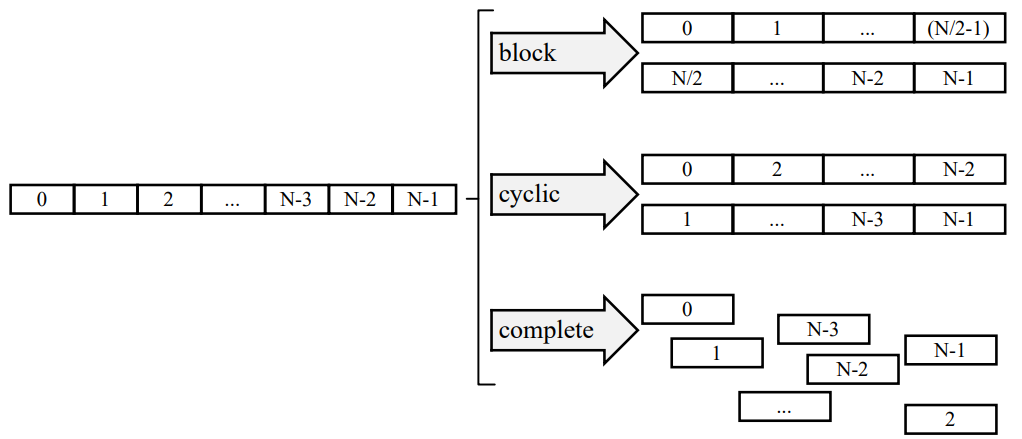
\includegraphics[width=1\textwidth]{solutions/loop_unrolling/partitioning.png}
    \caption{HLS Array Partitioning}
\end{figure}

Pertanto, è possibile elencare qui di seguito le soluzioni hardware progettate per l'approccio del parallelismo:
\begin{itemize}
    \item Unrolling Manuale Fattore=2
    \item Unrolling Manuale Fattore=4
    \item Unrolling Automatico Fattore=2
    \item Unrolling Automatico Fattore=4
    \item Unrolling Automatico con Partitioning Fattore=2
    \item Unrolling Automatico con Partitioning Fattore=4
\end{itemize}

\begin{figure}[H]
    \centering
    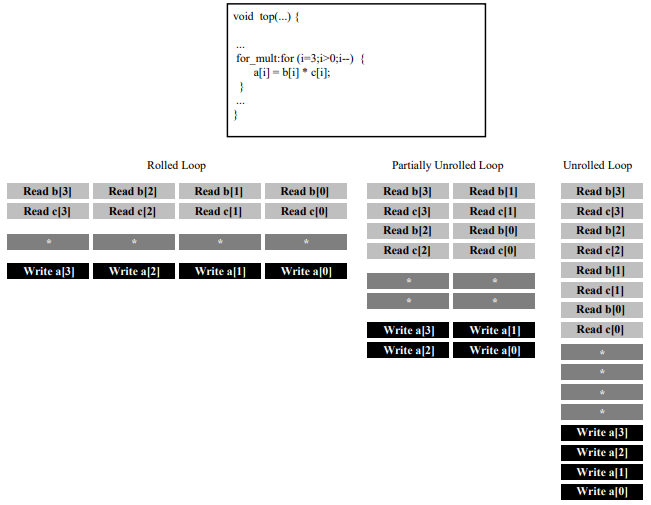
\includegraphics[width=1\textwidth]{solutions/loop_unrolling/unrolling.png}
    \caption{HLS Loop Unrolling}
\end{figure}

A questo proposito, verranno analizzati i report considerando le soluzioni hardware aventi stesso fattore così da poter effettuare confronti adeguati tra le varie implementazioni.In particolare, è stato considerato un loop unrolling di fattore 2 e un fattore 4. Ovviamente, la figura sopra allegata è solo un esempio per rappresentare meglio il concetto di unrolling e partitioning.

\subsubsection{Loop Unrolling Factor=2}
\lstinputlisting[language=C++]{solutions/loop_unrolling/factor2/fir_loop_unrolling_manual_factor2.cpp}
\lstinputlisting[language=C++]{solutions/loop_unrolling/factor2/fir_loop_unrolling_automatic_factor2.cpp}
\lstinputlisting[language=C++]{solutions/loop_unrolling/factor2/fir_loop_unrolling_automatic_partiotioning_factor2.cpp}

\begin{table}[H]
    \centering
    \begin{tabular}{|c|c|c|c|c|}
        \hline
        \textbf{Solution} & \textbf{Clock} & \textbf{Target} & \textbf{Estimated} & \textbf{Uncertainty} \\
        \hline
        Manuale & ap\_clk & 10.00 & 8.510 & 1.25 \\
        \hline
        Automatico & ap\_clk & 10.00 & 8.510 & 1.25 \\
        \hline
        Automatico con Partitioning & ap\_clk & 10.00 & 8.510 & 1.25 \\
        \hline
    \end{tabular}
    \caption{HLS Loop Unrolling Factor=2 Solution Timing Summary (ns)}
    \label{tab:hls-loop-unrolling-factor2-solution-timing-summary}
\end{table}

Si può notare come la latenza associata alla soluzione hardware basata su unrolling manuale sia la medesima di quella basata su unrolling automatico (effettuato mediante pragma). Questo è dovuto al fatto che l'implementazione è la stessa: nel primo caso è effettuato manualmente mentre nel secondo caso è effettuato mediante direttiva proprietaria del tool. Invece, nel caso della soluzione hardware basata su unrolling automatico e partitioning, si riscontra una latenza maggiore. Questo risultato è dovuto al fatto che, tramite il pragma di partizionamento, si è dovuto gestire, inoltre, letture e scritture in parallelo.

\begin{table}[H]
    \centering
    \begin{tabular}{|c|c|c|c|c|}
        \hline
        \multicolumn{1}{|c|}{\textbf{Solution}} & \multicolumn{2}{|c|}{\textbf{Latency}} & \multicolumn{2}{|c|}{\textbf{Interval}} \\
        & min & max & min & max \\
        \hline
        Manuale & 56 & 56 & 56 & 56 \\
        \hline
        Automatico & 56 & 56 & 56 & 56 \\
        \hline
        Automatico con Partitioning & 61 & 66 & 61 & 66 \\
        \hline
    \end{tabular}
    \caption{HLS Loop Unrolling Factor=2 Solution Latency Summary (clock cycles)}
    \label{tab:hls-loop-unrolling-factor2-solution-latency-summary}
\end{table}

Si può evidenziare come, nel caso della soluzione hardware con urolling automatico e partizionamento, l'aumento della latenza si ha soltanto in corrispondenza del loop di shifting, cioè proprio dove è stato collocato il pragma di partitioning.

\begin{table}[H]
    \centering
    \begin{tabular}{|c|c|c|c|c|c|c|c|c|c|}
        \hline
        \multicolumn{1}{|c|}{\textbf{Solution}} & \multicolumn{1}{|c|}{Loop Name} & \multicolumn{2}{|c|}{\textbf{Latency}} & \multicolumn{2}{c|}{\textbf{Iteration Latency}} & \multicolumn{2}{c|}{\textbf{Initiation Interval}} & \multicolumn{1}{c|}{\textbf{Trip}}  \\
        &  & min & max & min & max & achieved & target & \textbf{Count} \\
        \hline
        Manuale & - loopShifting & 10 & 10 & 2 & 2 & - & - & 5 \\
        & - loopAccumulator & 44 & 44 & 4 & 4 & - & - & 11 \\
        \hline
        Automatico & - loopShifting & 10 & 10 & 2 & 2 & - & - & 5 \\
        & - loopAccumulator & 44 & 44 & 4 & 4 & - & - & 11 \\
        \hline
        Automatico  & - loopShifting & 15 & 20 & 3 & 4 & - & - & 5 \\
        con Partitioning & - loopAccumulator & 44 & 44 & 4 & 4 & - & - & 11 \\
        \hline
    \end{tabular}
    \caption{HLS Loop Unrolling Factor=2 Solution Latency Loops Summary }
    \label{tab:hls-loop-unrolling-factor2-solution-loop-summary}
\end{table}

Aprendo la sezione Analysis del tool si può vedere meglio nel dettaglio che, all'interno del loop di shifting, sono presenti 2 shifting in parallelo (dal momento che è stato considerato un fattore di parallelismo pari a 2) sia peer la soluzione hardware di unrolling manuale sia per quella di unrolling automatico (mediante pragma).

\begin{figure}[H]
    \centering
    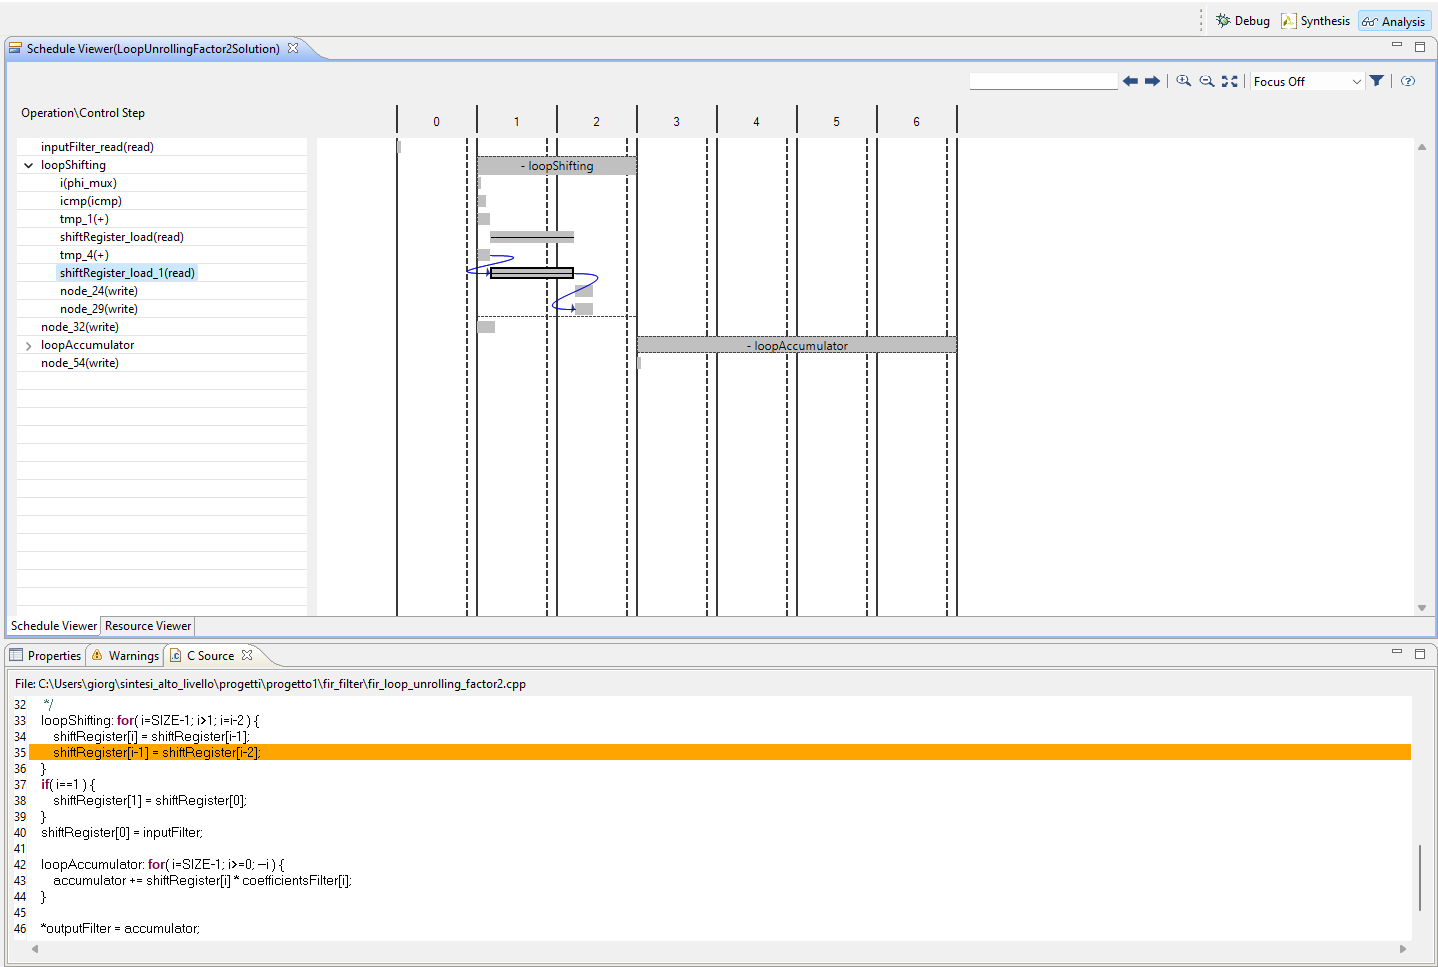
\includegraphics[width=0.9\textwidth]{solutions/loop_unrolling/factor2/loopunrollingmanual2.png}
    \caption{HLS Loop Unrolling Manual Factor=2 Analysis}
\end{figure}

\begin{figure}[H]
    \centering
    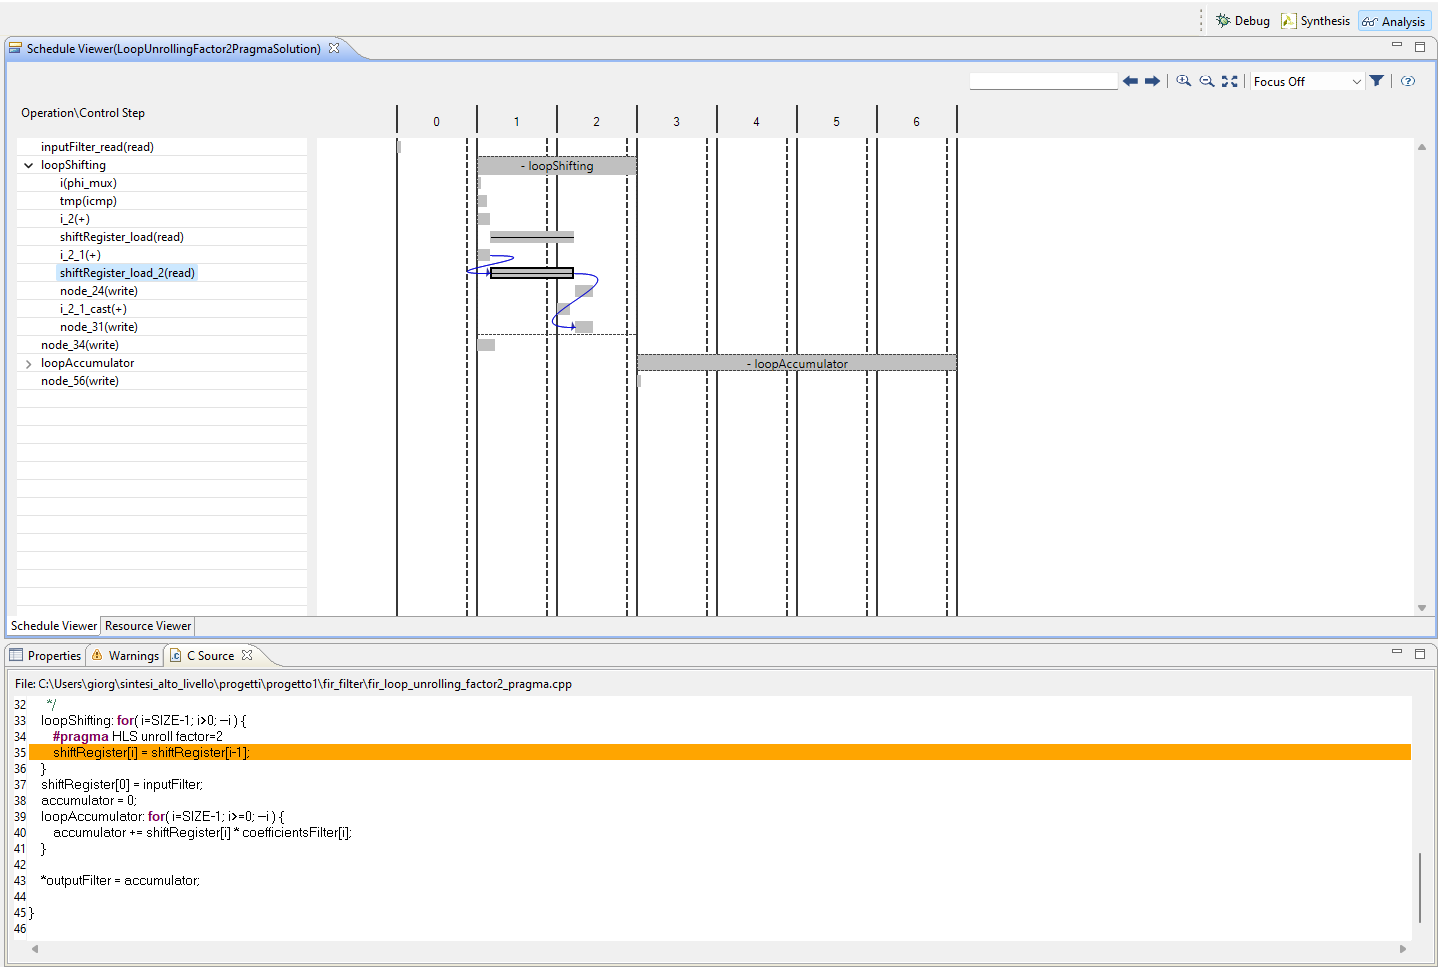
\includegraphics[width=0.9\textwidth]{solutions/loop_unrolling/factor2/loopunrollingautomatic2.png}
    \caption{HLS Loop Unrolling Automatic Factor=2 Analysis}
\end{figure}

Analizzando nel dettaglio il report si può notare come il numero di DSP e LUT sia pressocché il medesimo per tutte e tre le soluzioni hardware proposte. Per quanto riguarda, invece, il numero di BRAM utilizzate, le soluzioni basate su unrolling manuale e automatico presentano un'utilizzazione pari a 2, mentre quella basta su unrolling automatico e partitioning presenta un numero di BRAM utilizzato pari a 0. Questo è dovuto al fatto che il pragma di partizionamento, al fine di garantire accessi di read/write in memoria in parallelo, impone di non utilizzare le BRAM dual-port (che limiterebbero tali accessi). In particolare, impostando la tipologia di partizionamento \textit{complete}, la direttiva fa in modo che la soluzione hardware impieghi come memoria dei singoli registri, cosí che siano garantiti gli accessi in memoria in parallelo. Tanto è vero che si può notare un aumento considerevole dei FF in corrispondenza dell'architettura basata su unrolling automatico e partizionamento.

\begin{table}[H]
    \centering
    \begin{tabular}{|c|c|c|c|c|}
        \hline
        \textbf{Solution} & \textbf{BRAM\_18K} & \textbf{DSP48E} & \textbf{FF} & \textbf{LUT} \\
        \hline
        Manuale & 2 & 2 & 145 & 236 \\
        \hline
        Automatico & 2 & 2 & 141 & 251 \\
        \hline
        Automatico con Partitioning & 0 & 2 & 912 & 289 \\
        \hline
    \end{tabular}
    \caption{HLS Loop Unrolling Factor=2 Solution Utilization Estimates [\#]}
    \label{tab:hls-loop-unrolling-factor2-solution-utilization-report}
\end{table}

Qui di seguito vengono riportati i report relativi alla C/RTL Cosimulation, dove è possibile analizzare il numero di cicli di clock che servono per ottenere un risultato in uscita, e quello relativo a Export RTL.

\begin{table}[H]
    \centering
    \begin{tabular}{|c|c|c|c|c|c|c|c|c|}
        \hline
        \multicolumn{1}{|c|}{\textbf{Solution}} & \multicolumn{1}{|c|}{RTL} & \multicolumn{1}{|c|}{Status} & \multicolumn{3}{c|}{\textbf{Latency}} & \multicolumn{3}{c|}{\textbf{Interval}} \\
        & &  & min & avg & max & min & avg & max \\
        \hline
        Manuale & VHDL & Pass & 56 & 56 & 57 & 56 & 56 & 57 \\
        \hline
        Automatico & VHDL & Pass & 56 & 56 & 57 & 56 & 56 & 57 \\
        \hline
        Automatico con Partitioning & VHDL & Pass & 65 & 65 & 66 & 65 & 65 & 66 \\
        \hline
    \end{tabular}
    \caption{HLS Loop Unrolling Factor=2 Solution C/RTL Cosimulation Report }
    \label{tab:hls-loop-unrolling-factor2-solution-cosimulation-report}
\end{table}

\begin{table}[H]
    \centering
    \begin{tabular}{|c|c|c|c|c|c|c|c|c|}
        \hline
        \textbf{Solution} & \textbf{SLICE} & \textbf{LUT} & \textbf{FF} & \textbf{DSP} & \textbf{BRAM} & \textbf{CP} & \textbf{CP} & \textbf{CP} \\
        & & & & & & \textbf{required} & \textbf{achieved} & \textbf{achieved}\\
        & & & & & & & \textbf{post-} & \textbf{post-}\\
        & & & & & & & \textbf{synthesis} & \textbf{implementation}\\
        \hline
        Manuale & 31 & 97 & 72 & 2 & 2 & 10 & 5.745 & 5.692 \\
        \hline
        Automatico & 29 & 97 & 72 & 2 & 2 & 10 & 5.745 & 5.692 \\
        \hline
        Automatico  & 294 & 413 & 843 & 2 & 0 & 10 & 5.745 & 6.188 \\
        con Partitioning & & & & & & & & \\
        \hline
    \end{tabular}
    \caption{HLS Loop Unrolling Factor=2 Solution Export RTL Report}
    \label{tab:vivado-loop-unrolling-factor2-solution-export-rtl-report}
\end{table}


Pertanto, importando l'IP in Vivado e impostando un clock constraint pari a 10ns è possibile analizzare i seguenti report di risorse, timing, potenza dinamica ed energia per singola operazione.
\lstinputlisting[language=VHDL]{solutions/loop_unrolling/factor2/clk_constraint.xdc}

Analizzando il report di utilizzazione delle risorse generato da Vivado dopo aver effettuato il processo di implementazione, è possibile notare come il numero di risorse stimato dal tool HLS è leggermente mutato. Però, si può evidenziare come il cambiamento delle risorse tra le varie soluzioni hardware è il medesimo, cioè il numero di LUT e FF nel caso dell'implementazione con unrolling automatico e partitioning sia aumentato considerevolmente e il numero di BRAM si è ridotto a zero.

\begin{table}[H]
    \centering
    \begin{tabular}{|c|c|c|c|c|c|c|c|}
        \hline
        \textbf{Solution} & \textbf{LUT} & \textbf{LUTRAM} & \textbf{FF} & \textbf{BRAM} & \textbf{DSP} & \textbf{IO} & \textbf{BUFG} \\
        \hline
        Manuale & 98 & 0 & 72 & 1 & 2 & 71 & 1 \\
        \hline
        Automatico & 98 & 0 & 72 & 1 & 2 & 71 & 1 \\
        \hline
        Automatico & 413 & 0 & 843 & 0 & 2 & 71 & 1 \\
        con Partitioning & & & & & & & \\
        \hline
    \end{tabular}
    \caption{Vivado Loop Unrolling Factor=2 Solution Utilization Report [\#]}
    \label{tab:vivado-loop-unrolling-factor2-utilization-report}
\end{table}

Si è, inoltre, analizzato l'utilizzazione delle risorse effettuando un confronto con la soluzione hardware basata sulla scissione del loop dal momento che tali architetture basate su unrolling sono basate sulla prima citata. In particolare, si può notare come il numero di risorse utilizzate sia pressoché il medesimo tra la soluzione hardware basta su loop fission e quelle basate rispettivamente sull'unrolling manuale e automatico di fattore 2. Più nello specifico, considerando le implementazioni basate sul parallelismo manuale e automatico rispetto a quella basta sul loop fission, il numero di LUT è diminuito di circa il $40\%$, il numero di FF è diminuito di circa il $32\%$ e il numero di BRAM è aumentato di un'unità. Invece, effettuando un confronto tra quella basata su partitioning e quella basata sulla scissione del loop, il numero di LUT è aumentato di circa il $161\%$ e il numero di FF di circa il $695\%$.

\begin{figure}[H]
    \centering
    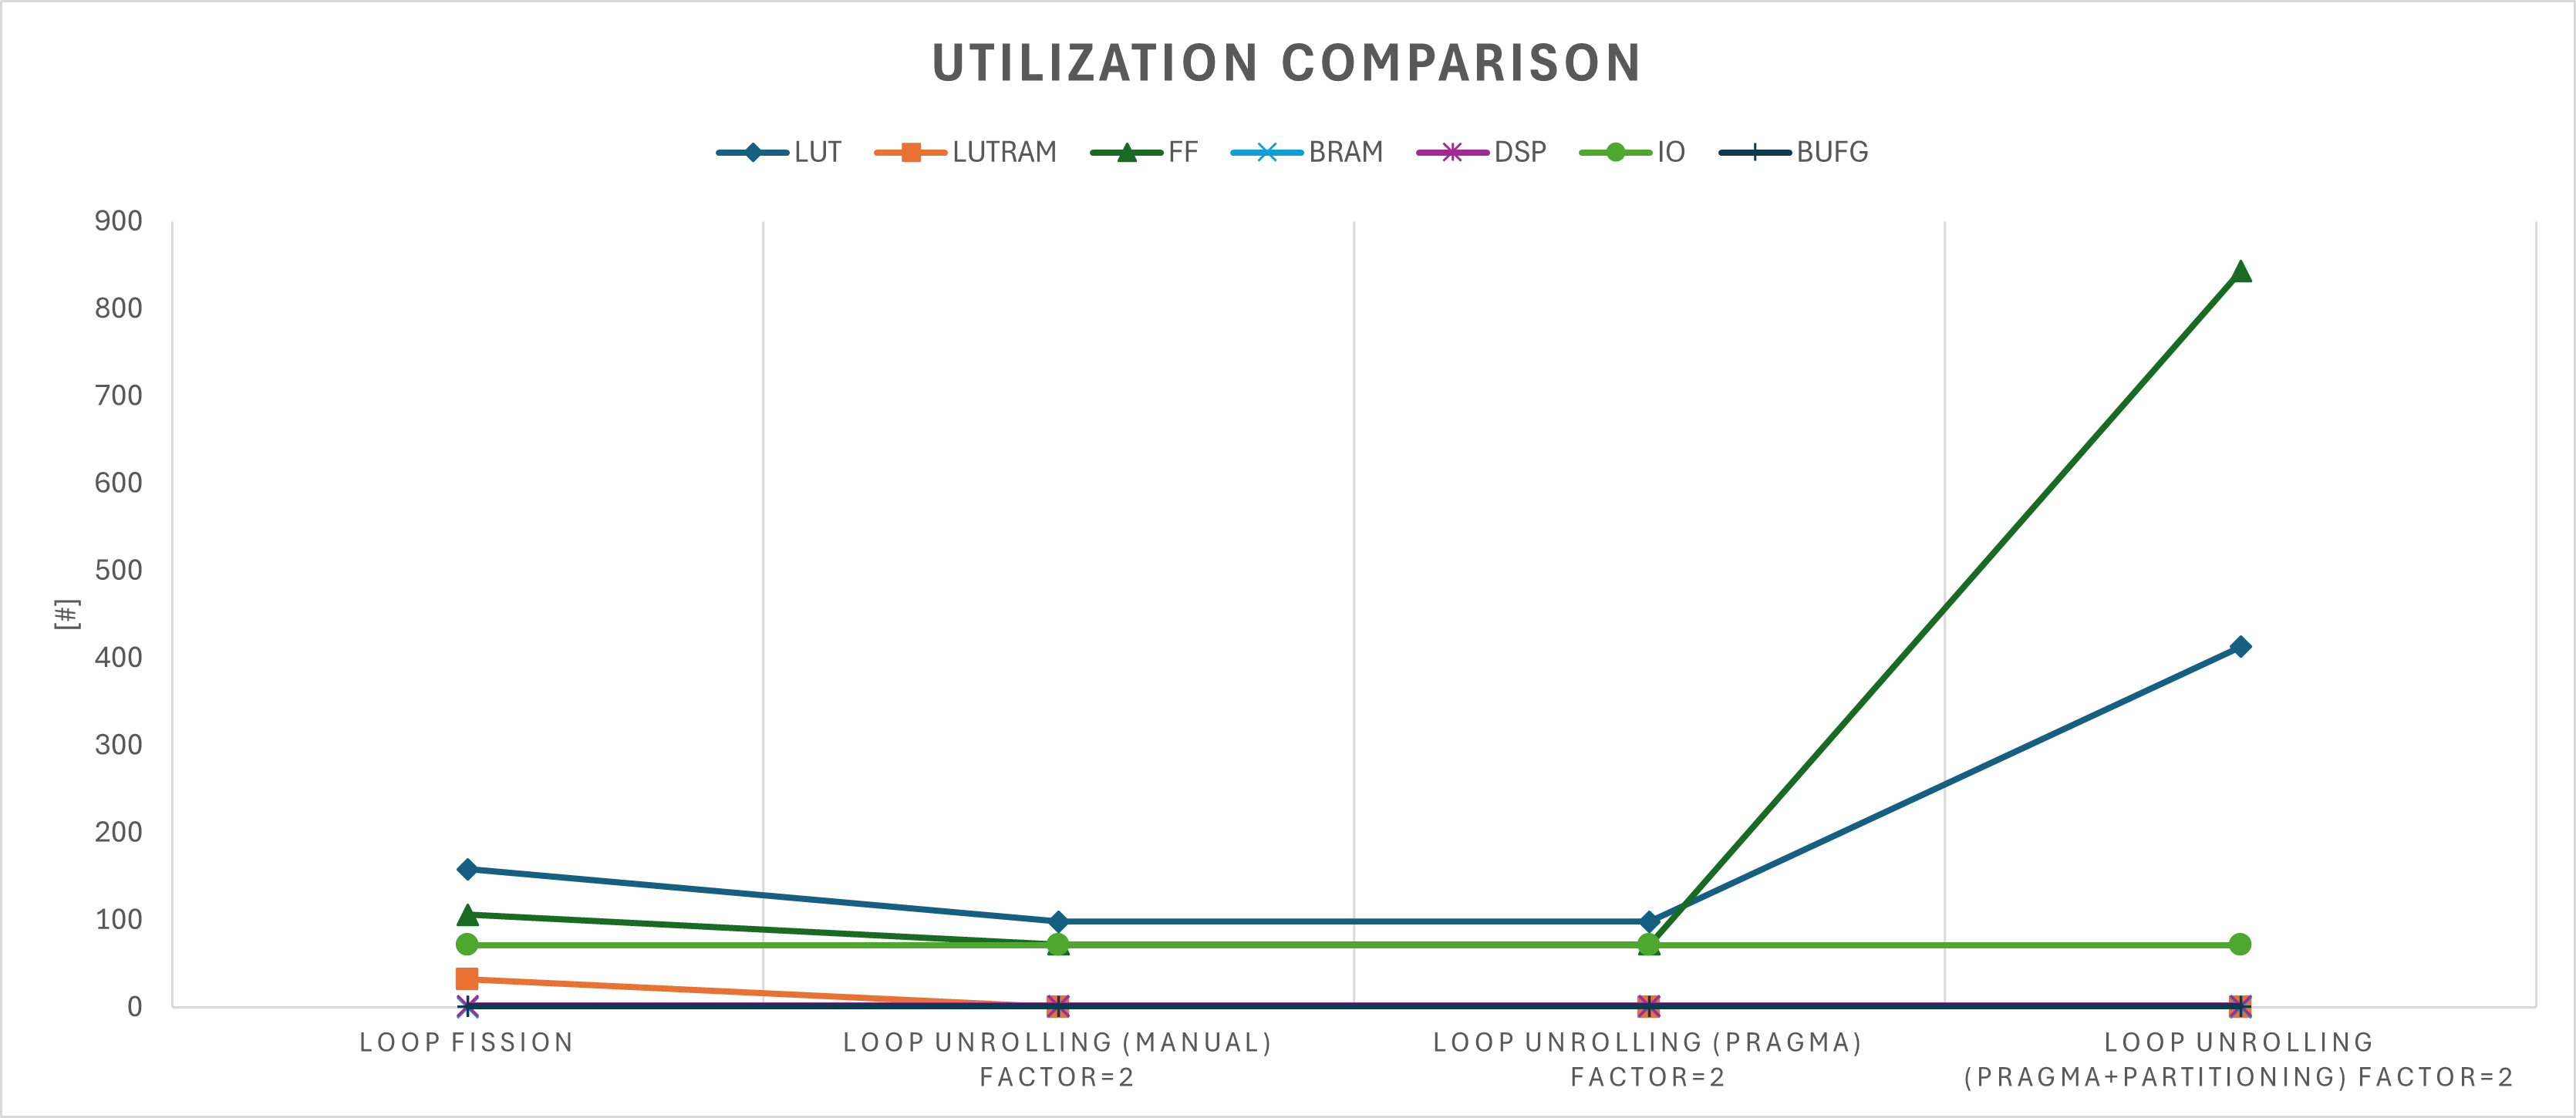
\includegraphics[width=0.9\textwidth]{solutions/loop_unrolling/factor2/loopunrollingfactor2utilization.png}
    \caption{Vivado Loop Unrolling Factor=2 Utilization Plot}
    \label{fig:vivado-loop-unrolling-factor2-utilization-plot}
\end{figure}

Infine, per quanto riguarda il timing, è possibile notare come il numero di cicli sia pressocché il medesimo tra la soluzione basata su unrolling manuale e quella basata su unrolling automatico. Invece, come precedentemente citato, la soluzione basata su partizionamento presenta un numero di cicli di clock, tali per garantire un risultato, maggiore.

\begin{table}[H]
    \centering
    \begin{tabular}{|c|c|c|c|c|}
        \hline
        \textbf{Solution} & \textbf{Cycles} [\#] & \textbf{Clock Constraint} [ns] & \textbf{WNS} [ns] & \textbf{Maximum Clock} \\
        & & & & \textbf{Frequency} [MHz] \\
        \hline
        Manuale & 57 & 10 & 4.33 & 176.366843 \\
        \hline
        Automatico & 57 & 10 & 4.33 & 176.366843 \\
        \hline
        Automatico & 66 & 10 & 3.469 & 153.1159087 \\
        con Partitioning & & & & \\
        \hline
    \end{tabular}
    \caption{Vivado Loop Unrolling Factor=2 Solution Timing Report}
    \label{tab:vivado-loop-unrolling-factor2-solution-timing-report}
\end{table}

Effettuando un confronto grafico e tenendo conto anche della soluzione basata sulla scissione del loop, è possibile evidenziare un numero di cicli di clock, tali per garantire un risultato, un WNS e una maximum clock frequency pressoché uguali tra l'implementazione basata su loop fission e quella basata su partizionamento. Questo accade dal momento che la soluzione hardware basata su unrolling automatico e partitioning fa diminuire il numero di cicli di clock tramite il parallelismo e lo fa aumentare allo stesso tempo a causa del partizionamento. 

\begin{figure}[H]
    \centering
    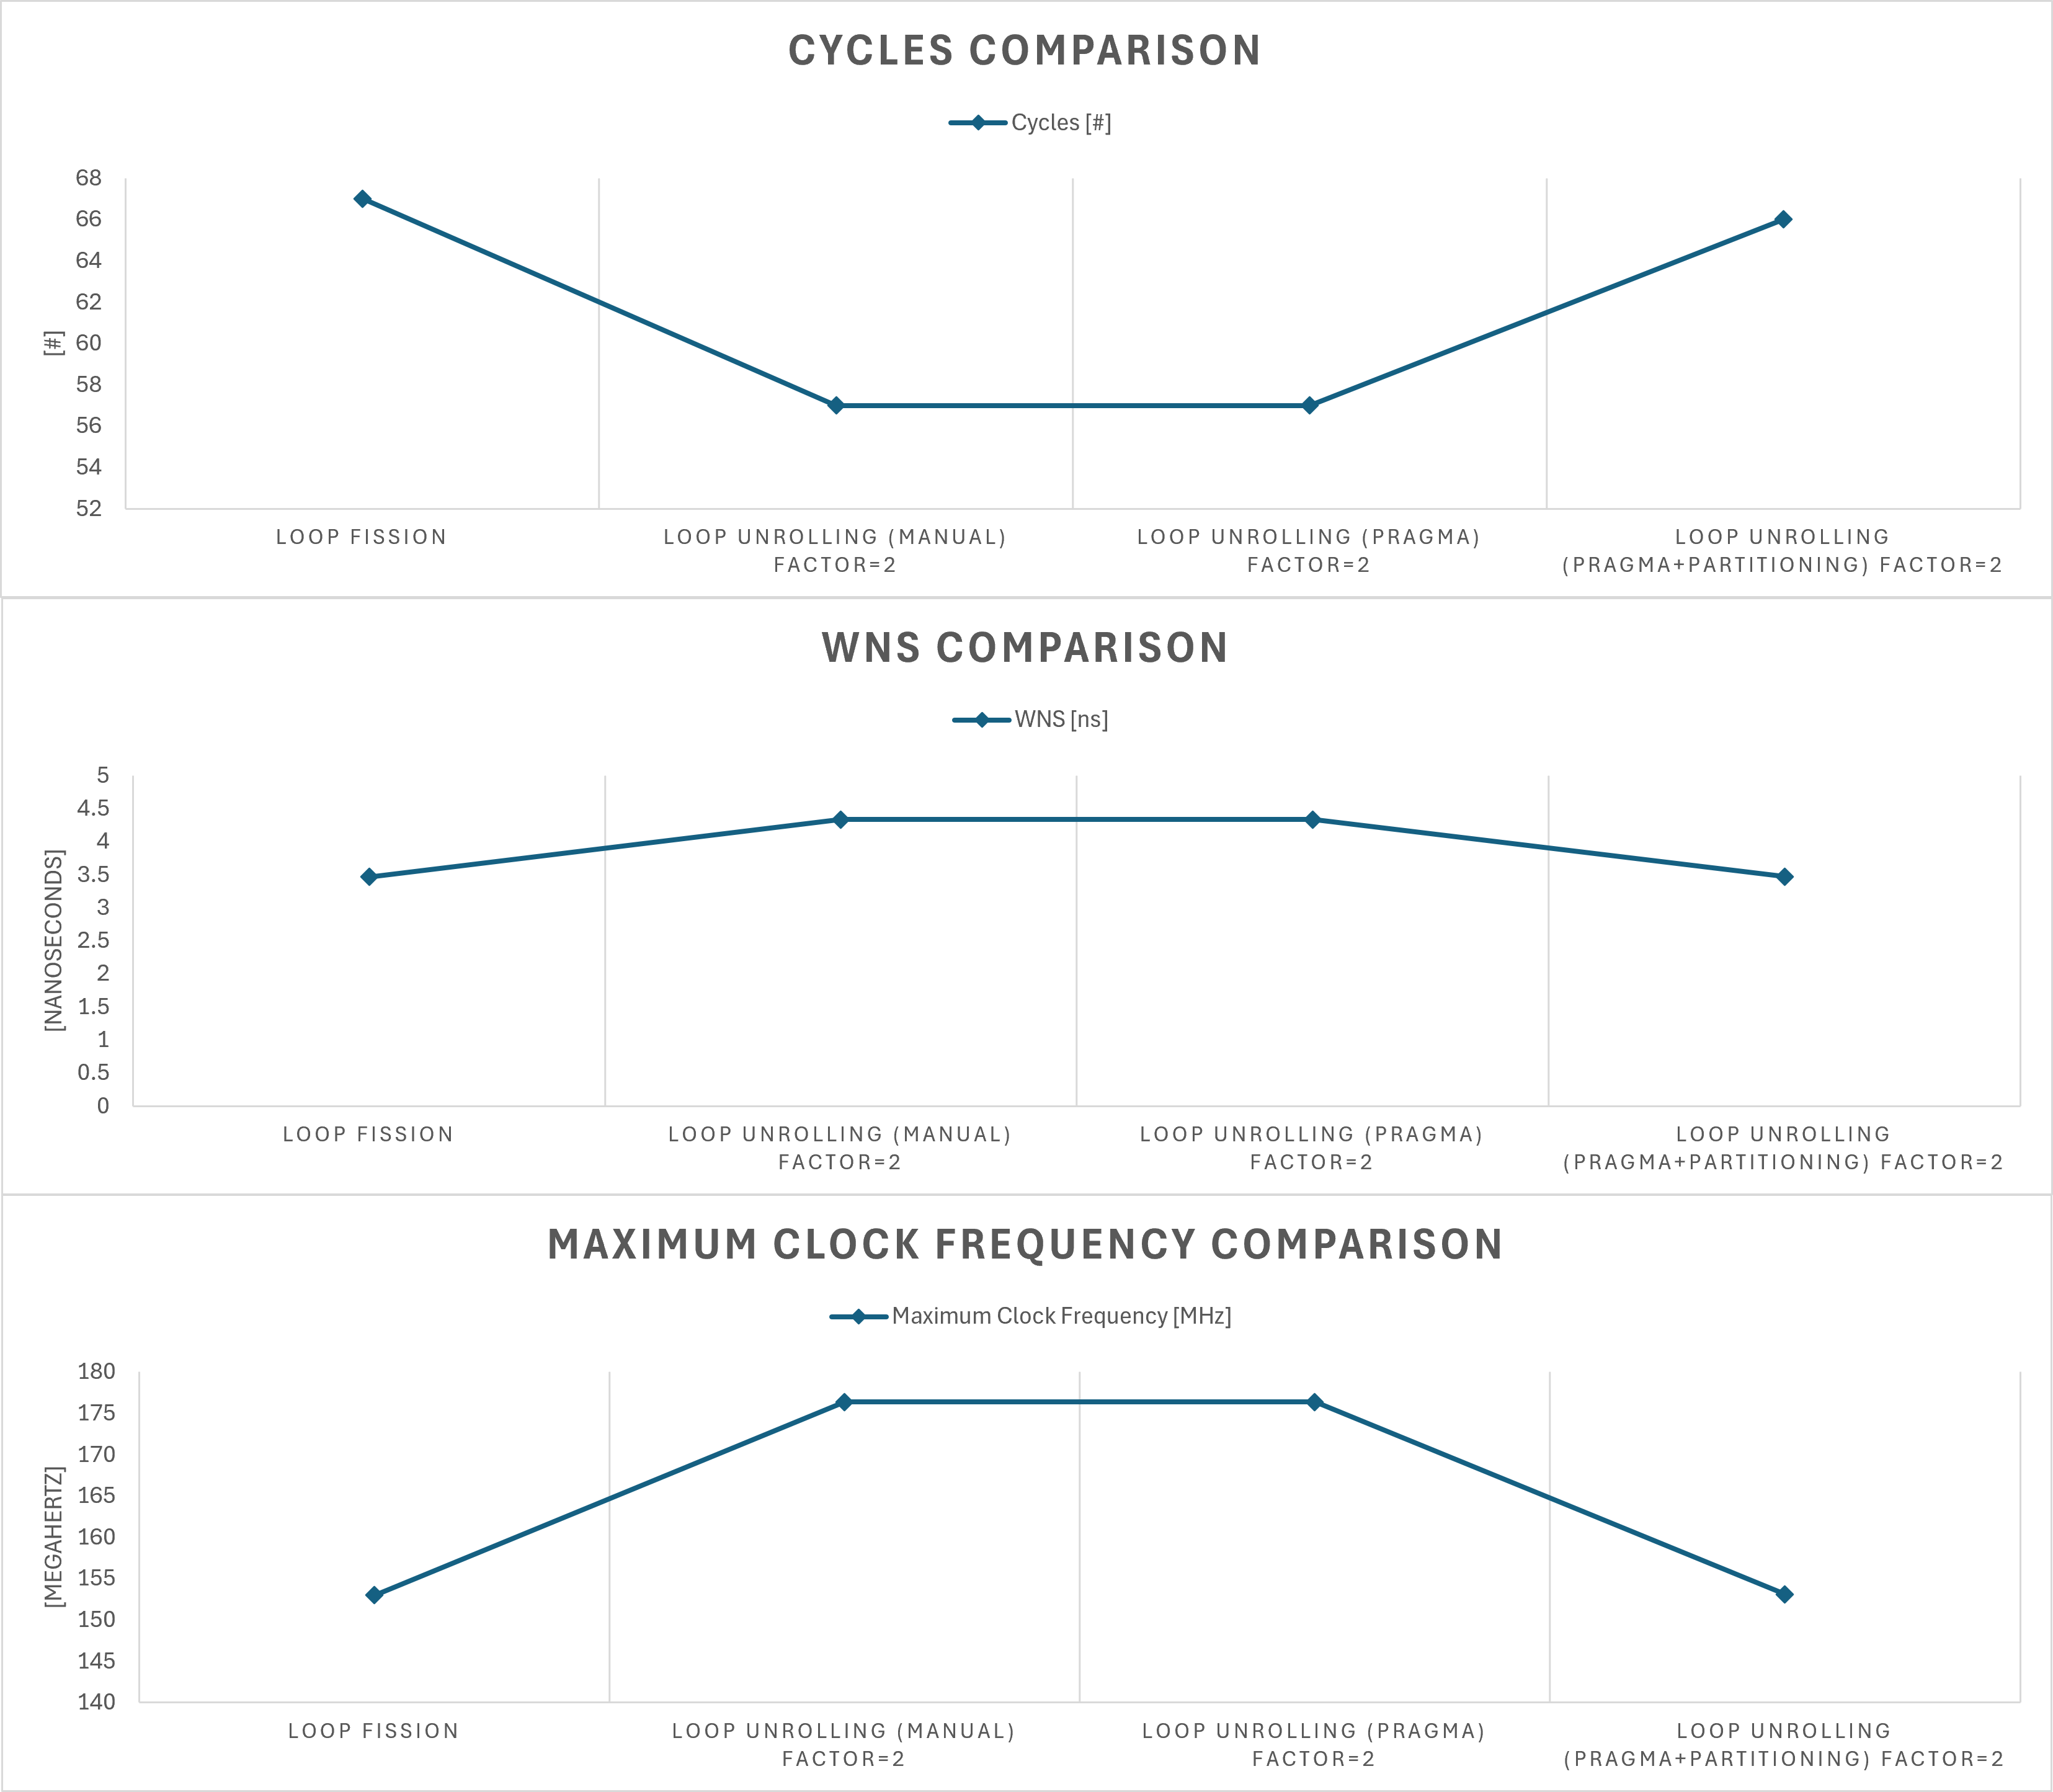
\includegraphics[width=0.8\textwidth]{solutions/loop_unrolling/factor2/loopunrollingfactor2timing.png}
    \caption{Vivado Loop Unrolling Factor=2 Timing Plot}
    \label{fig:vivado-loop-unrolling-factor2-solution-timing-plot}
\end{figure}

Per quanto riguarda, invece, la potenza dinamica associata alle tre soluzioni hardware proposte in questa sezione, è possibile notare come i contributi associati al Clock Enable e Clocks risultano essere notevolmente più grandi in corrispondenza dell'implementazione basata su partizionamento. Questo potrebbe essere causato dal notevole aumento dell'utilizzazione dei FF per questa solution. 

\begin{table}[H]
    \centering
    \begin{tabular}{|c|c|c|c|c|c|c|c|}
        \hline
        \textbf{Solution} & \textbf{BRAM} & \textbf{Clock} & \textbf{Clocks} & \textbf{DSP} & \textbf{Logic} & \textbf{Set/}& \textbf{Data} \\
        & & \textbf{Enable} & & & & \textbf{Reset} & \\
        \hline
        Manuale & 1.250551548 & 0.096387172 & 0.900532817 & 0.268251897 & 0.260709843 & 0.003146866 & 0.423992984 \\
        \hline
        Automatico & 1.240851358 & 0.082524632 & 0.960682868 & 0.272355421 & 0.266662013 & 0.00428147 & 0.425589533 \\
        \hline
        Automatico & & & & & & & \\
        con & 0 & 0.325270201 & 2.352835611 & 0.263715046 & 0.575191109 & 0.007010513 & 0.750690058 \\
        Partitioning & & & & & & & \\
        \hline
    \end{tabular}
    \caption{Vivado Loop Unrolling Factor=2 Solution Dynamic Power Report [mW]}
    \label{tab:vivado-loop-unrolling-factor2-solution-dynamic-power-reproot}
\end{table}

Infatti, è possibile riscontrare un aumento della potenza dinamica totale e dell'energia per singola operazione in corrispondenza dell'architettura basata su unrolling e partitioning. Invece, per quanto riguarda le altre due solution (unrolling manuale e automatico), entrambi i parametri appena citati risultano essere i medesimi. 

\begin{table}[H]
    \centering
    \begin{minipage}[t]{0.45\linewidth}
        \centering
        \begin{tabular}{|c|c|}
            \hline
            \textbf{Solution} & \textbf{Dynamic Total} \\
            \hline
            Manuale & 3.203573127 \\
            \hline
            Automatico & 3.252947294 \\
            \hline
            Automatico & 4.274712538 \\
            con Partitioning & \\
            \hline
        \end{tabular}
        \caption{Vivado Loop Unrolling Factor=2 Solution Dynamic Power Report [mW]}
        \label{tab:vivado-loop-unrolling-factor2-solution-dynamic-power-reproot}
    \end{minipage}
    \hfill
    \centering
    \begin{minipage}[t]{0.45\linewidth}
        \centering
        \begin{tabular}{|c|c|}
            \hline
            \textbf{Solution} & \textbf{Energy Single Operation} \\
            \hline
            Manuale & 32.03573127 \\
            \hline
            Automatico & 32.52947294 \\
            \hline
            Automatico & 42.74712538 \\
            con Partitioning & \\
            \hline
        \end{tabular}
        \caption{Vivado Loop Unrolling Factor=2 Solution Energy Single Operation Report [pJ]}
        \label{tab:vivado-loop-unrolling-factor2-solution-solution-energy-single-operation-reproot}
    \end{minipage}
\end{table}

Analizzando graficamente queste tre soluzioni e in aggiunta anche l'implementazione basata sulla scissione del loop, è possibile notare come quella basasta su loop fission presenta un medesimo valore di potenza dinamica totale ed energia per singola operazione rispetto alle due soluzioni di unrolling manuale e automatico.

\begin{figure}[H]
    \centering
    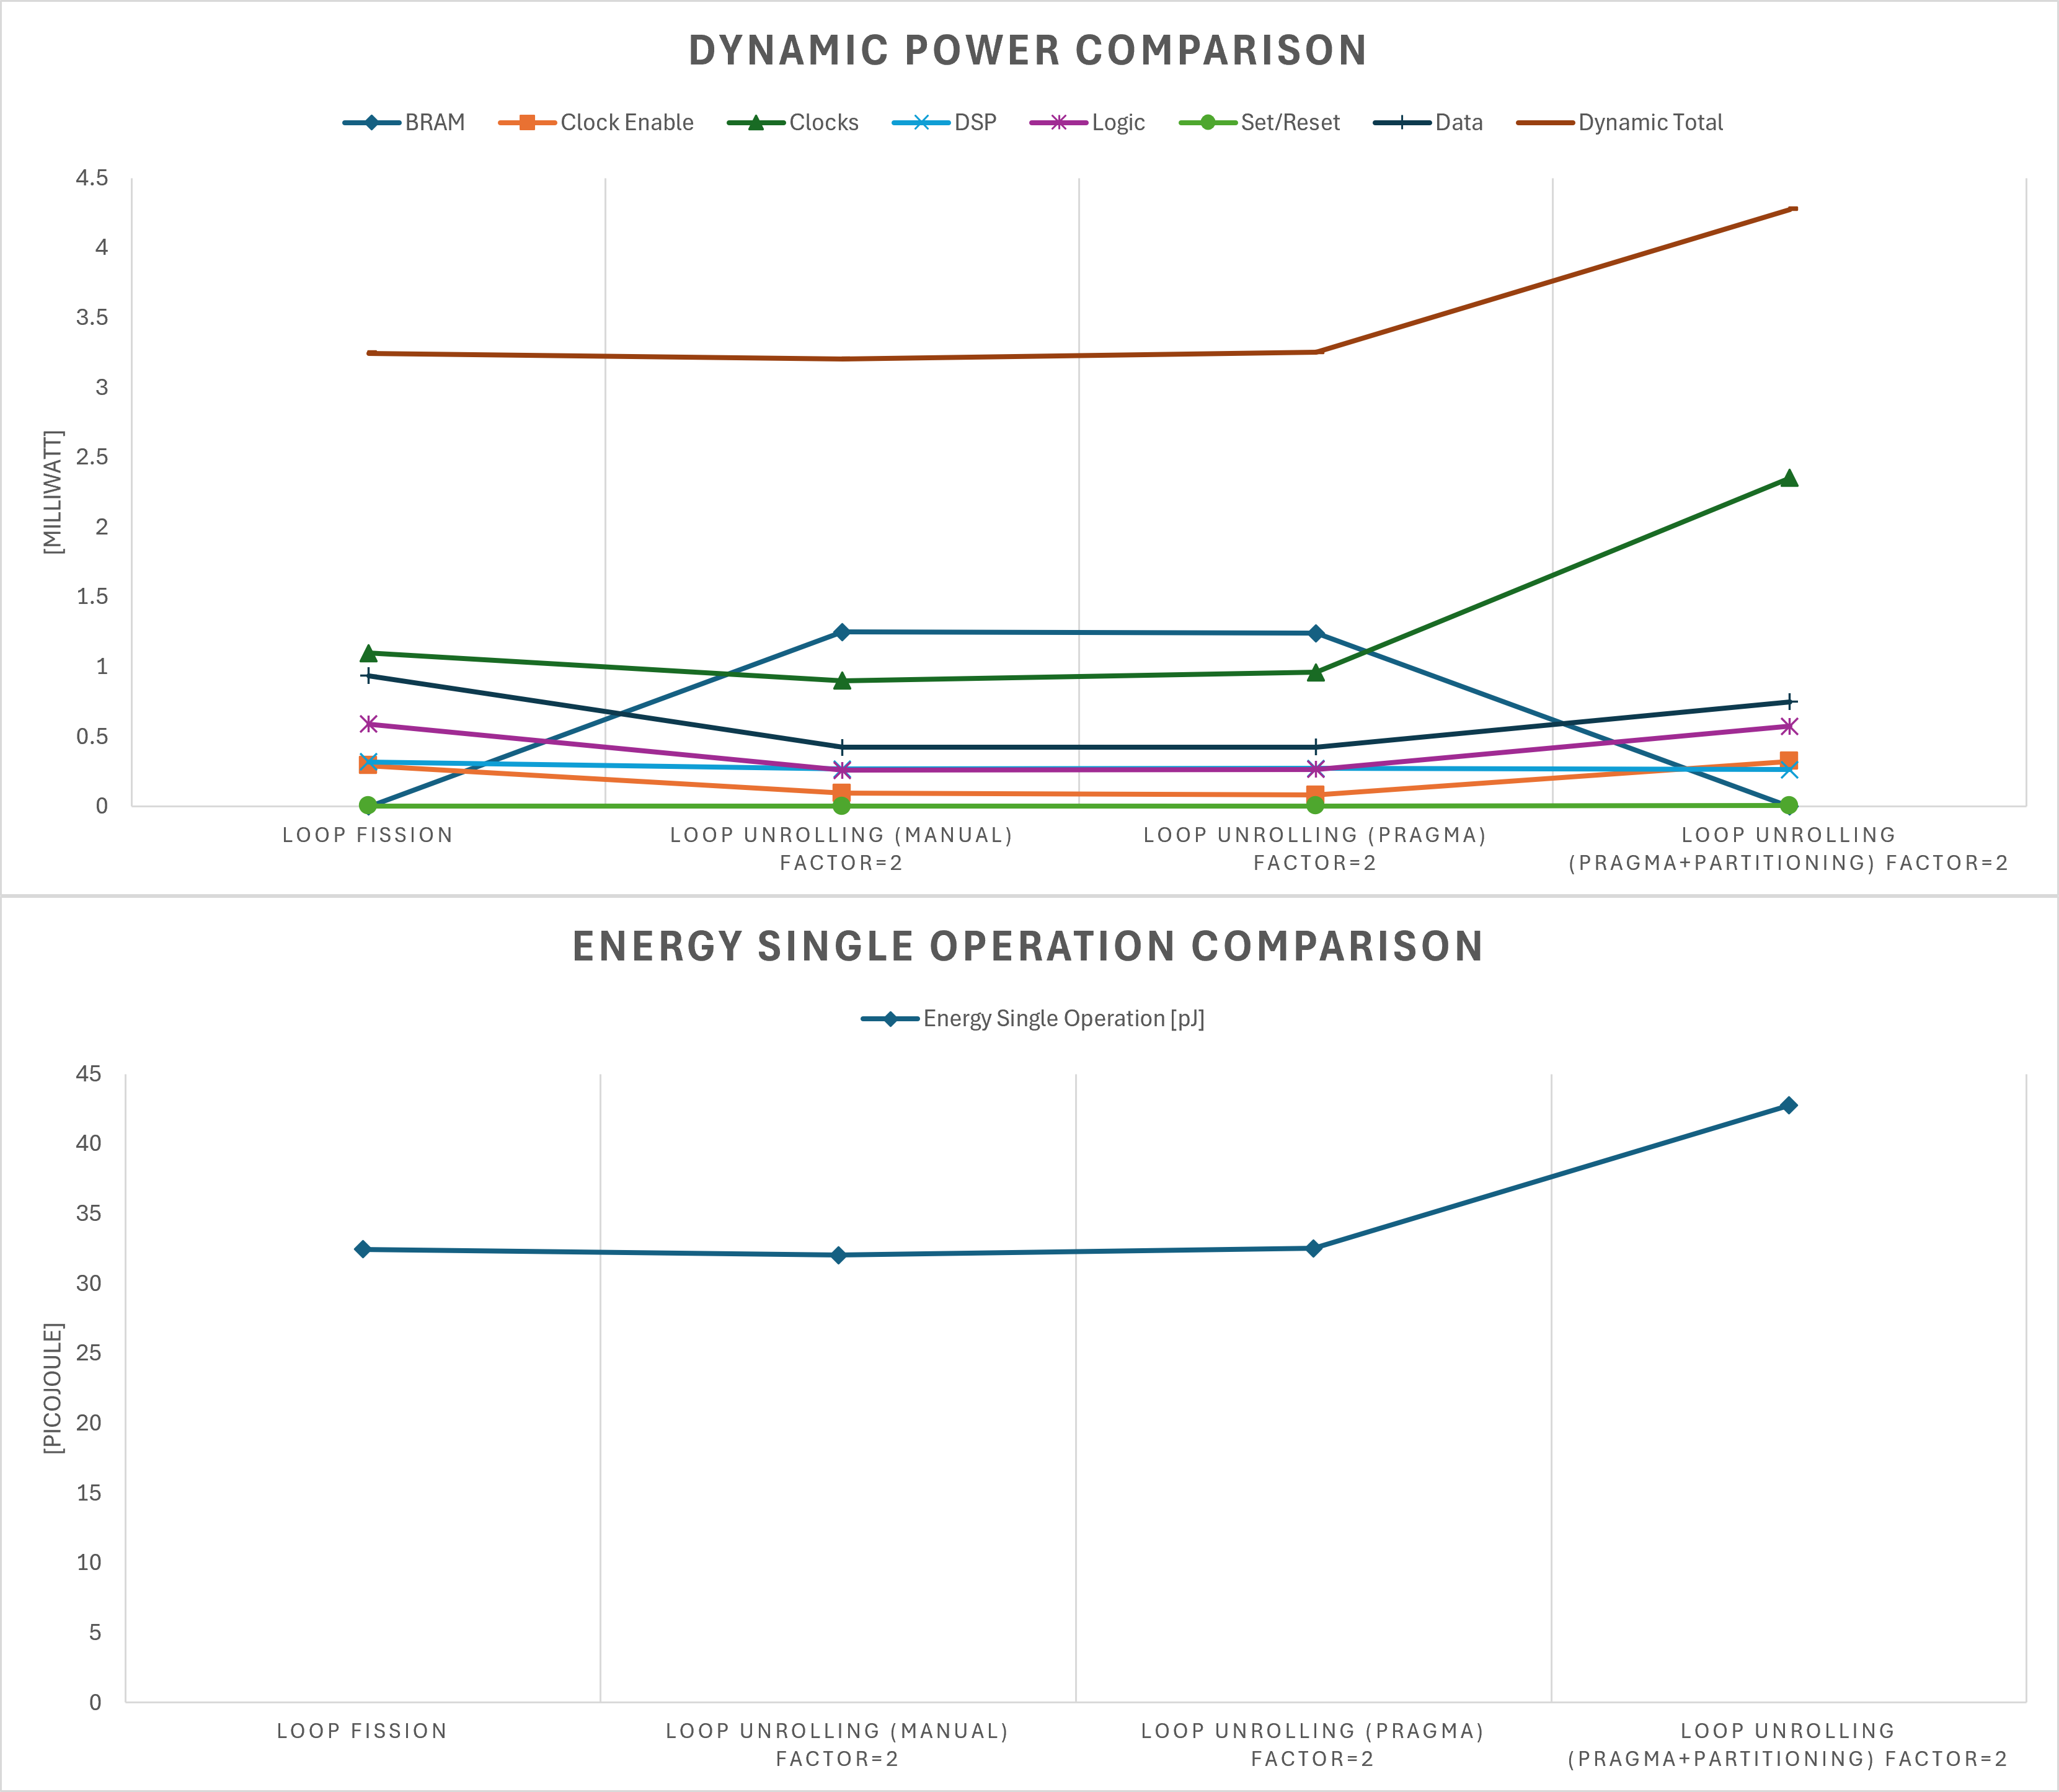
\includegraphics[width=\textwidth]{solutions/loop_unrolling/factor2/loopunrollingfactor2power.png}
    \caption{Vivado Loop Unrolling Factor=2 Dynamic Power Plot}
    \label{fig:vivado-loop-unrolling-factor2-solution-power-plot}
\end{figure}


\newpage

\subsubsection{Loop Unrolling Factor=4}
\lstinputlisting[language=C++]{solutions/loop_unrolling/factor4/fir_loop_unrolling_manual_factor4.cpp}
\lstinputlisting[language=C++]{solutions/loop_unrolling/factor4/fir_loop_unrolling_automatic_factor4.cpp}
\lstinputlisting[language=C++]{solutions/loop_unrolling/factor4/fir_loop_unrolling_automatic_partiotioning_factor4.cpp}

\begin{table}[H]
    \centering
    \begin{tabular}{|c|c|c|c|c|}
        \hline
        \textbf{Solution} & \textbf{Clock} & \textbf{Target} & \textbf{Estimated} & \textbf{Uncertainty} \\
        \hline
        Manuale & ap\_clk & 10.00 & 8.510 & 1.25 \\
        \hline
        Automatico & ap\_clk & 10.00 & 8.510 & 1.25 \\
        \hline
        Automatico con Partitioning & ap\_clk & 10.00 & 8.510 & 1.25 \\
        \hline
    \end{tabular}
    \caption{HLS Loop Unrolling Factor=4 Solution Timing Summary (ns)}
    \label{tab:hls-loop-unrolling-factor4-solution-timing-summary}
\end{table}

\begin{table}[H]
    \centering
    \begin{tabular}{|c|c|c|c|c|}
        \hline
        \multicolumn{1}{|c|}{\textbf{Solution}} & \multicolumn{2}{|c|}{\textbf{Latency}} & \multicolumn{2}{|c|}{\textbf{Interval}} \\
        & min & max & min & max \\
        \hline
        Manuale & 58 & 58 & 58 & 58 \\
        \hline
        Automatico & 62 & 66 & 62 & 66 \\
        \hline
        Automatico con Partitioning & 62 & 64 & 62 & 64 \\
        \hline
    \end{tabular}
    \caption{HLS Loop Unrolling Factor=4 Solution Latency Summary (clock cycles)}
    \label{tab:hls-loop-unrolling-factor4-solution-latency-summary}
\end{table}

\begin{table}[H]
    \centering
    \begin{tabular}{|c|c|c|c|c|c|c|c|c|c|}
        \hline
        \multicolumn{1}{|c|}{\textbf{Solution}} & \multicolumn{1}{|c|}{Loop Name} & \multicolumn{2}{|c|}{\textbf{Latency}} & \multicolumn{2}{c|}{\textbf{Iteration Latency}} & \multicolumn{2}{c|}{\textbf{Initiation Interval}} & \multicolumn{1}{c|}{\textbf{Trip}}  \\
        &  & min & max & min & max & achieved & target & \textbf{Count} \\
        \hline
        Manuale & - loopShifting & 12 & 12 & 4 & 4 & - & - & 3 \\
        & - loopAccumulator & 44 & 44 & 4 & 4 & - & - & 11 \\
        \hline
        Automatico & - loopShifting & 15 & 18 & 5 & 5 & - & - & 3 \\
        & - loopAccumulator & 44 & 44 & 4 & 4 & - & - & 11 \\
        \hline
        Automatico  & - loopShifting & 15 & 17 & 5 & 5 & - & - & 3 \\
        con Partitioning & - loopAccumulator & 44 & 44 & 4 & 4 & - & - & 11 \\
        \hline
    \end{tabular}
    \caption{HLS Loop Unrolling Factor=4 Solution Latency Loops Summary }
    \label{tab:hls-loop-unrolling-factor4-solution-loop-summary}
\end{table}

In questo caso si può notare come il trip count sia, ovviamente, il medesimo per tutte e tre le soluzioni. Ciò che cambia effettivamente, come nel caso del fattore pari a 2, è la latency associata ai loop. In particolare, analizzando più nel dettaglio, tramite l'interfaccia Analysis, si può evidenziare come il loopShifting, in cui viene implementato un parallelismo pari a 4, viene gestito in maniera differente. Infatti, nel caso del loop unrolling manuale, vengono effettuate in parallelo due read alla volta e poi successivamente vengono eseguite in parallelo due write alla volta. Invece, nel caso della soluzione hardware basata su unrolling automatico, vengono effettuate una read e una write in parallelo per ogni ciclo di latenza. Nello specifico, considerando quattro shifting per ogni iterazione, viene effettuata la read al primo ciclo di latenza e, successivamente, viene eseguita la write corrispondente in parallelo alla read relativo al secondo shifting e così via. Di conseguenza, si avranno cinque colpi di latenza per ogni iterazione come riportato dal valore di iteration latency del report di sintesi.

\begin{figure}[H]
    \centering
    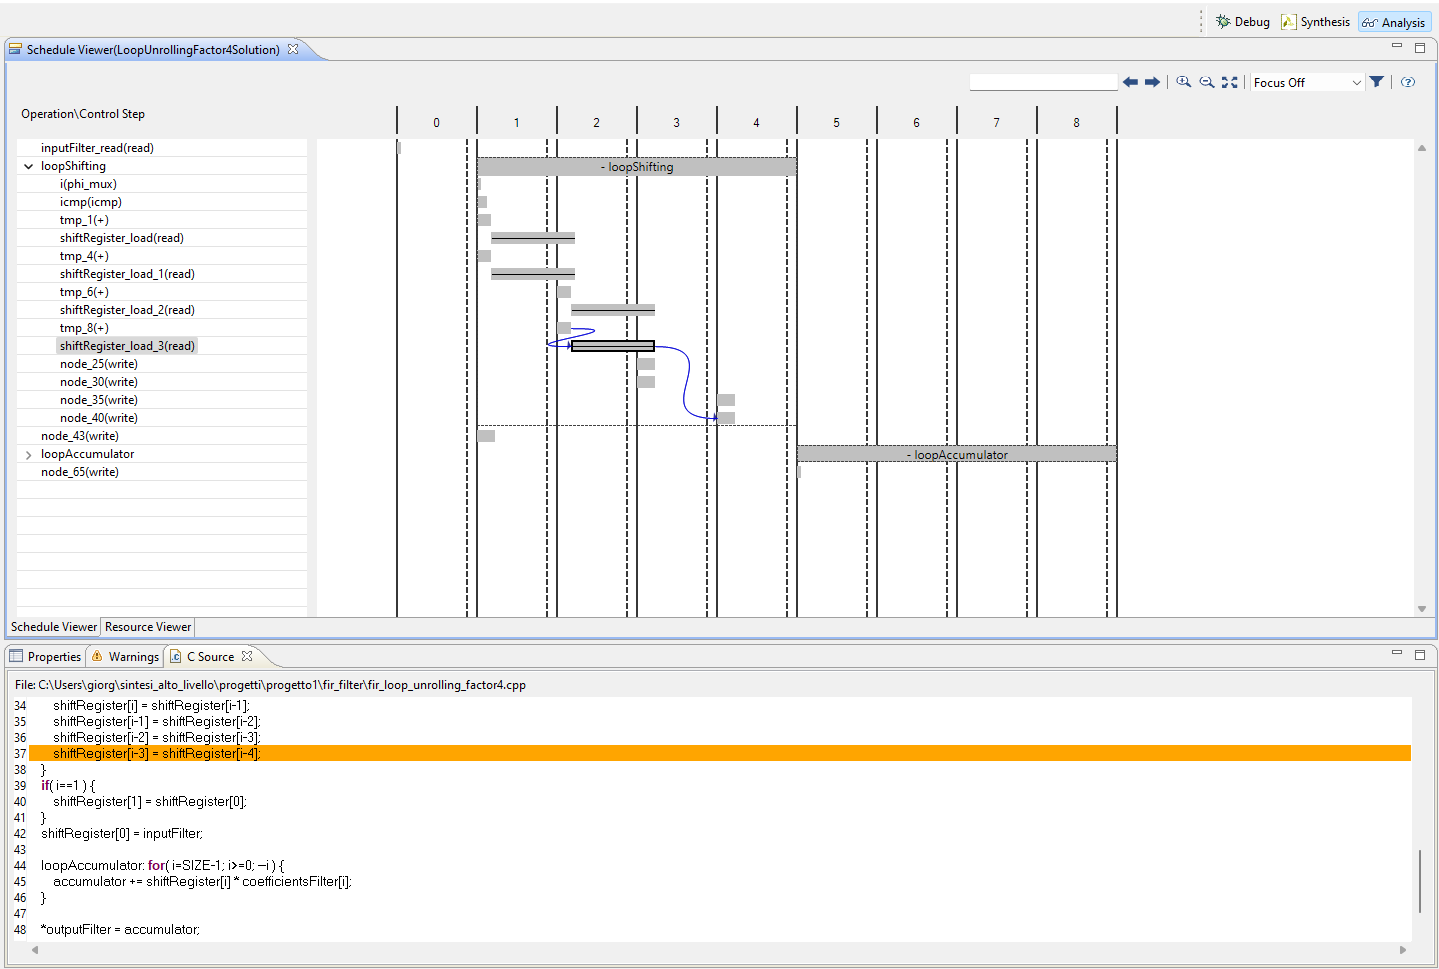
\includegraphics[width=0.9\textwidth]{solutions/loop_unrolling/factor4/loopunrollingmanual4.png}
    \caption{HLS Loop Unrolling Manual Factor=4 Analysis}
\end{figure}

\begin{figure}[H]
    \centering
    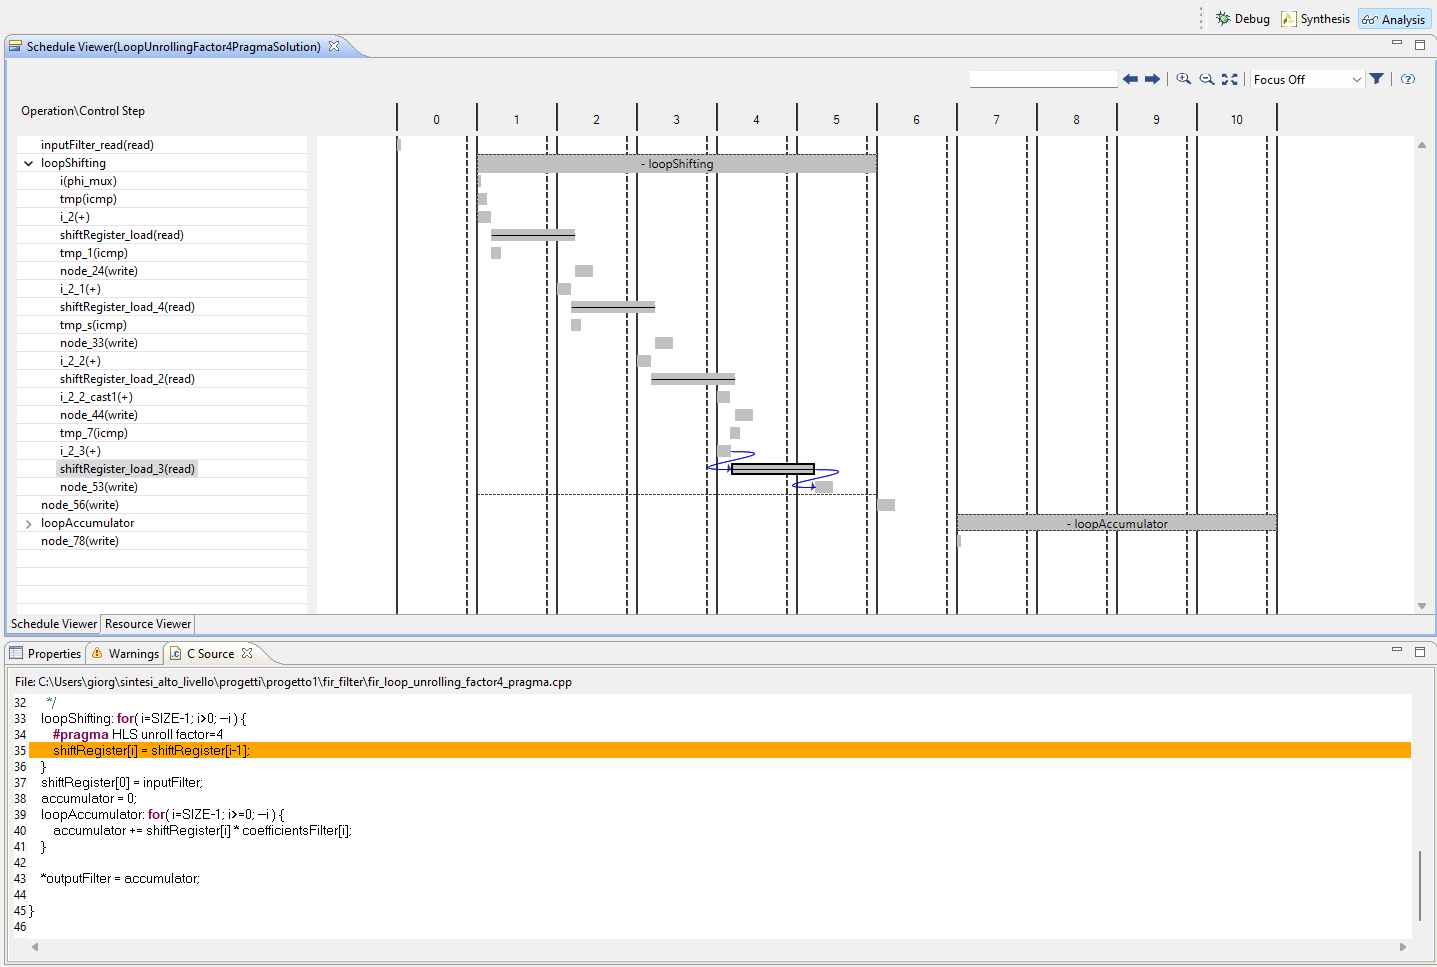
\includegraphics[width=0.9\textwidth]{solutions/loop_unrolling/factor4/loopunrollingautomatic4.png}
    \caption{HLS Loop Unrolling Automatic Factor=4 Analysis}
\end{figure}

Analogamente a quanto è stato analizzato e descritto nel caso di parallelismo di fattore pari a 2, anche in questo caso si può notare come l'utilizzazione delle risorse sia quasi la medesima tra il loop unrolling manuale e automatico. Invece, per quanto riguarda il loop unrolling automatico con partitioning, si ha un notevole aumento dell'utilizzazione sia di FF sia di LUT.

\begin{table}[H]
    \centering
    \begin{tabular}{|c|c|c|c|c|}
        \hline
        \textbf{Solution} & \textbf{BRAM\_18K} & \textbf{DSP48E} & \textbf{FF} & \textbf{LUT} \\
        \hline
        Manuale & 2 & 2 & 221 & 318 \\
        \hline
        Automatico & 2 & 2 & 194 & 367 \\
        \hline
        Automatico con Partitioning & 0 & 2 & 928 & 748 \\
        \hline
    \end{tabular}
    \caption{HLS Loop Unrolling Factor=4 Solution Utilization Estimates [\#]}
    \label{tab:vivado-loop-unrolling-factor4-solution-utilization-report}
\end{table}

Qui di seguito vengono riportati i report relativi alla C/RTL Cosimulation, dove è possibile analizzare il numero di cicli di clock che servono per ottenere un risultato in uscita, e quello relativo a Export RTL.

\begin{table}[H]
    \centering
    \begin{tabular}{|c|c|c|c|c|c|c|c|c|}
        \hline
        \multicolumn{1}{|c|}{\textbf{Solution}} & \multicolumn{1}{|c|}{RTL} & \multicolumn{1}{|c|}{Status} & \multicolumn{3}{c|}{\textbf{Latency}} & \multicolumn{3}{c|}{\textbf{Interval}} \\
        & &  & min & avg & max & min & avg & max \\
        \hline
        Manuale & VHDL & Pass & 58 & 58 & 59 & 58 & 58 & 59 \\
        \hline
        Automatico & VHDL & Pass & 60 & 60 & 61 & 60 & 60 & 61 \\
        \hline
        Automatico con Partitioning & VHDL & Pass & 58 & 58 & 59 & 58 & 58 & 59 \\
        \hline
    \end{tabular}
    \caption{HLS Loop Unrolling Factor=4 Solution C/RTL Cosimulation Report }
    \label{tab:hls-loop-unrolling-factor4-solution-cosimulation-report}
\end{table}

\begin{table}[H]
    \centering
    \begin{tabular}{|c|c|c|c|c|c|c|c|c|}
        \hline
        \textbf{Solution} & \textbf{SLICE} & \textbf{LUT} & \textbf{FF} & \textbf{DSP} & \textbf{BRAM} & \textbf{CP} & \textbf{CP} & \textbf{CP} \\
        & & & & & & \textbf{required} & \textbf{achieved} & \textbf{achieved}\\
        & & & & & & & \textbf{post-} & \textbf{post-}\\
        & & & & & & & \textbf{synthesis} & \textbf{implementation}\\
        \hline
        Manuale & 46 & 160 & 147 & 2 & 2 & 10 & 5.745 & 5.692 \\
        \hline
        Automatico & 40 & 145 & 93 & 2 & 2 & 10 & 5.745 & 5.692 \\
        \hline
        Automatico  & 412 & 1145 & 864 & 2 & 0 & 10 & 5.745 & 7.109 \\
        con Partitioning & & & & & & & & \\
        \hline
    \end{tabular}
    \caption{HLS Loop Unrolling Factor=4 Solution Export RTL Report}
    \label{tab:vivado-loop-unrolling-factor4-solution-export-rtl-report}
\end{table}

Pertanto, importando l'IP in Vivado e impostando un clock constraint pari a 10ns è possibile analizzare i seguenti report di risorse, timing, potenza dinamica ed energia per singola operazione.
\lstinputlisting[language=VHDL]{solutions/loop_unrolling/factor2/clk_constraint.xdc}

Analogamente all'unrolling di fattore pari a 2, anche in questo caso in corrispondenza della soluzione hardware basata su unrolling e partizionamento si ha un notevole aumento di utilizzazione delle risorse. Inoltre, si può notare come il numero di FF utilizzati per la solution di unrolling automatico risulta essere circa il $37\%$ in meno rispetto a quella basata su unrolling manuale. Evidentemente il tool, tramite la direttiva proprietaria, è riuscito ad effettuare delle ottimizzazione tali da garantire una diminuzione dei Flip Flop.

\begin{table}[H]
    \centering
    \begin{tabular}{|c|c|c|c|c|c|c|c|}
        \hline
        \textbf{Solution} & \textbf{LUT} & \textbf{LUTRAM} & \textbf{FF} & \textbf{BRAM} & \textbf{DSP} & \textbf{IO} & \textbf{BUFG} \\
        \hline
        Manuale & 159 & 0 & 147 & 1 & 2 & 71 & 1 \\
        \hline
        Automatico & 145 & 0 & 93 & 1 & 2 & 71 & 1 \\
        \hline
        Automatico & 1145 & 0 & 864 & 0 & 2 & 71 & 1 \\
        con Partitioning & & & & & & & \\
        \hline
    \end{tabular}
    \caption{Vivado Loop Unrolling Factor=4 Solution Utilization Report [\#]}
    \label{tab:vivado-loop-unrolling-factor4-utilization-report}
\end{table}

Effettuando un confronto grafico e tenendo conto dei dati precedentemente ottenuti per la soluzione basata su scissione del loop, si può notare come l'utilizzazione delle risorse sia pressocché la medesima tra loop fission e loop unrolling automatico.

\begin{figure}[H]
    \centering
    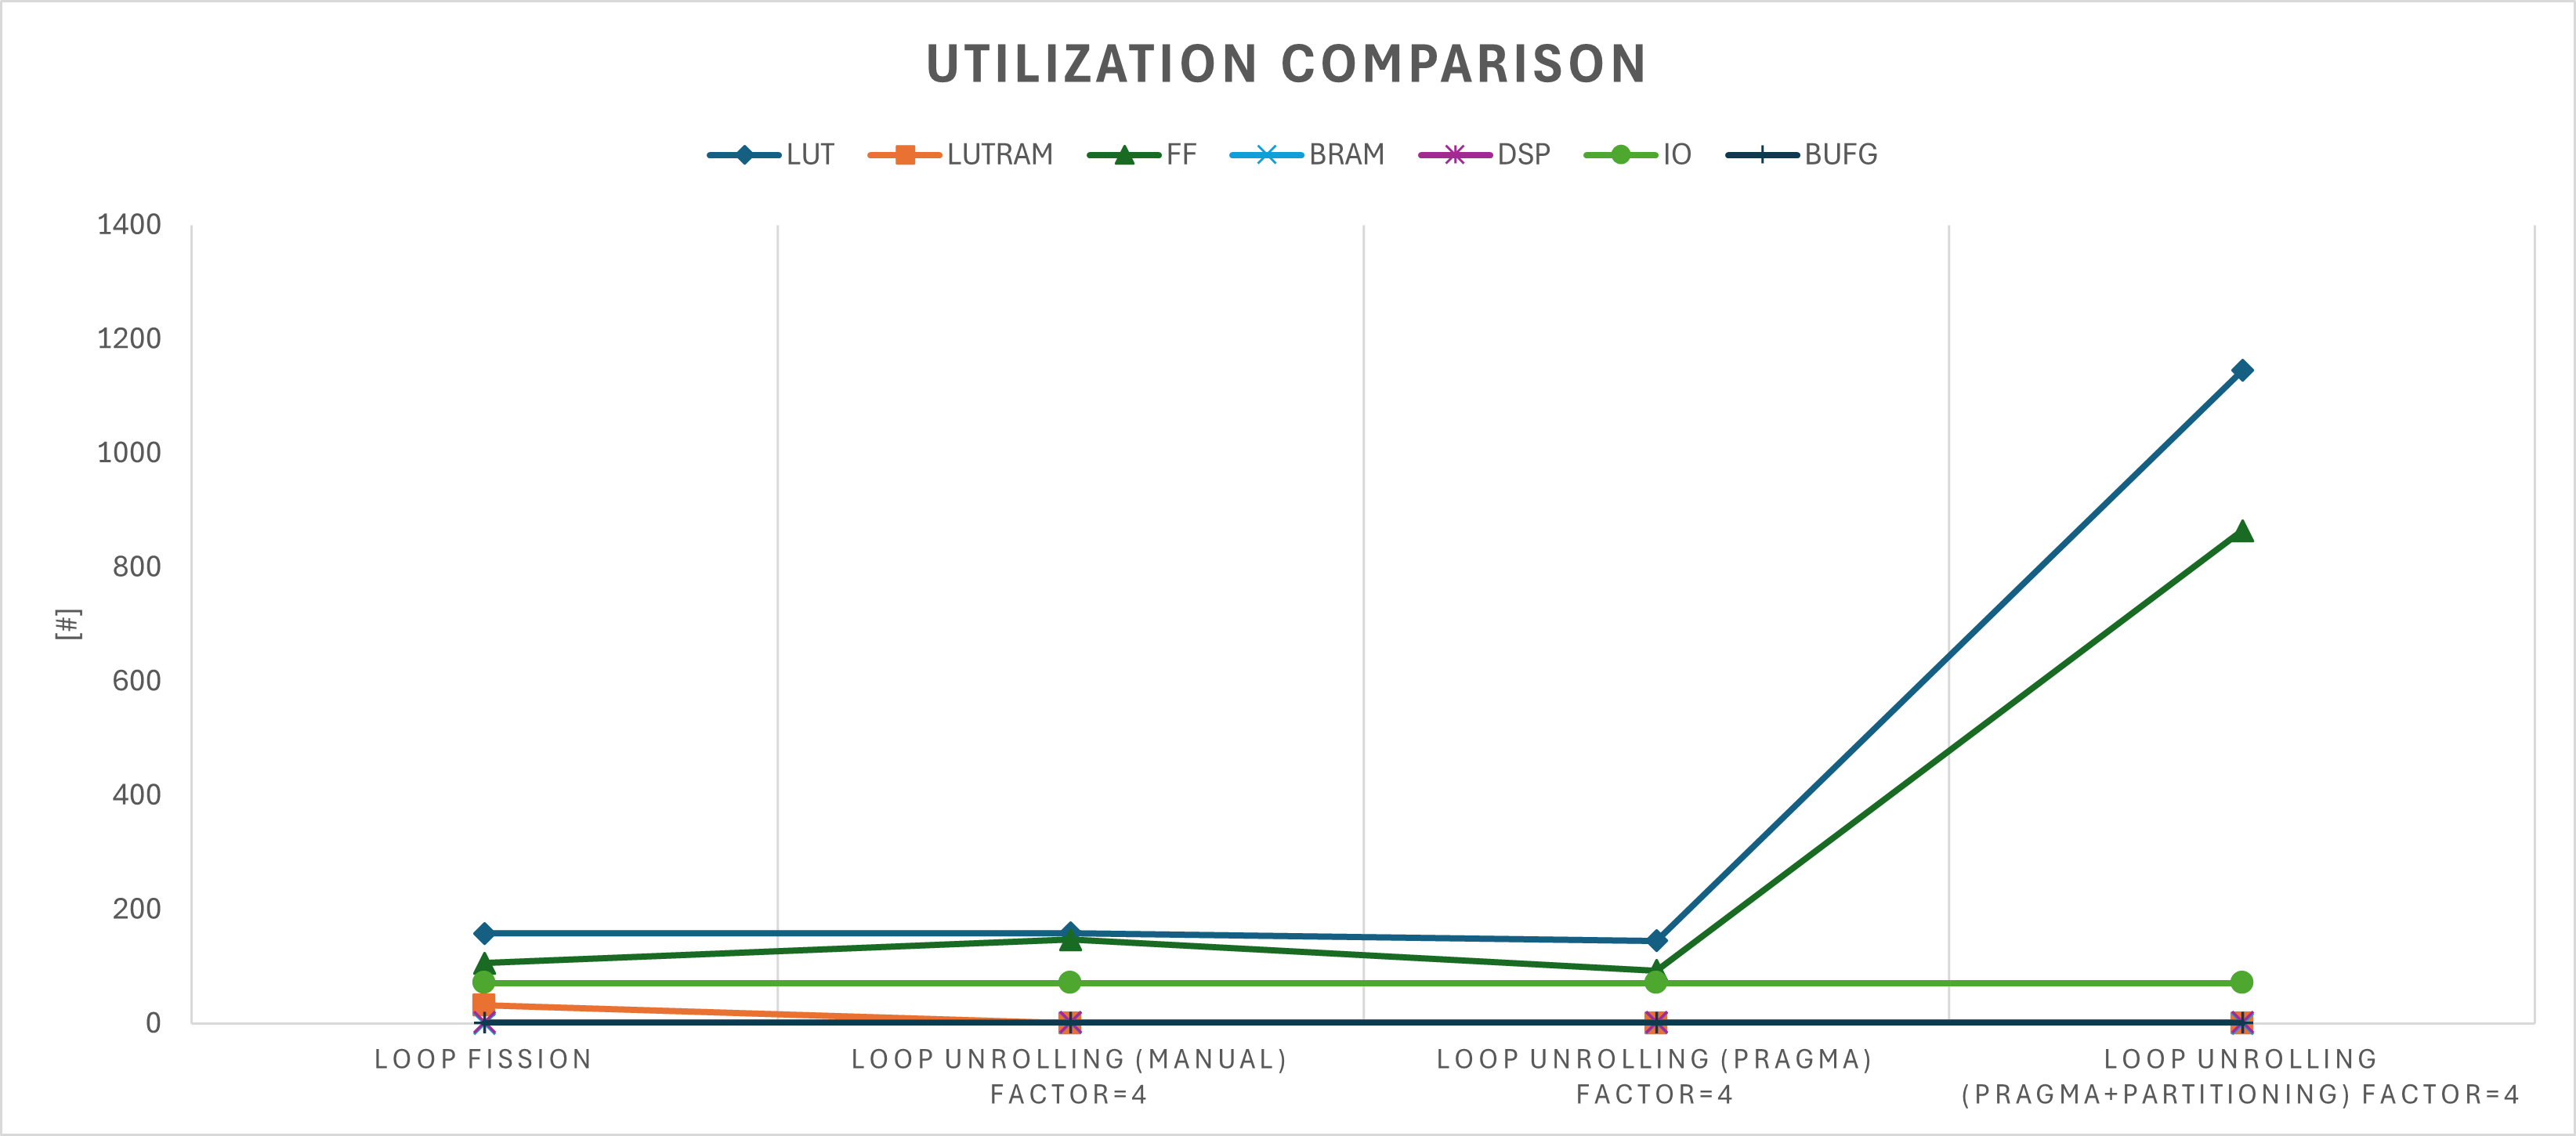
\includegraphics[width=0.9\textwidth]{solutions/loop_unrolling/factor4/loopunrollingfactor4utilization.png}
    \caption{Vivado Loop Unrolling Factor=4 Utilization Plot}
    \label{fig:vivado-loop-unrolling-factor4-utilization-plot}
\end{figure}

Per quanto riguarda il report di timing, è possibile notare, analogamente a quanto successo per l'unrolling di fattore pari a 2, una diminuzione della maximum clock frequency in corrispondenza della soluzione basata su loop unrolling automatico con partizionamento.

\begin{table}[H]
    \centering
    \begin{tabular}{|c|c|c|c|c|}
        \hline
        \textbf{Solution} & \textbf{Cycles} [\#] & \textbf{Clock Constraint} [ns] & \textbf{WNS} [ns] & \textbf{Maximum Clock} \\
        & & & & \textbf{Frequency} [MHz] \\
        \hline
        Manuale & 59 & 10 & 4.257 & 174.1250218 \\
        \hline
        Automatico & 61 & 10 & 4.33 & 176.366843 \\
        \hline
        Automatico & 59 & 10 & 3.097 & 144.8645516 \\
        con Partitioning & & & & \\
        \hline
    \end{tabular}
    \caption{Vivado Loop Unrolling Factor=4 Solution Timing Report}
    \label{tab:vivado-loop-unrolling-factor4-solution-timing-report}
\end{table}

Per quanto riguarda, invece, il numero di cicli di clock per garantire un risultato in uscita, in questo caso, per le tre soluzioni basate su unrolling di fattore pari a 4, si è ottenuto un valore minore rispetto alla soluzione basata su scissione del loop. 

\begin{figure}[H]
    \centering
    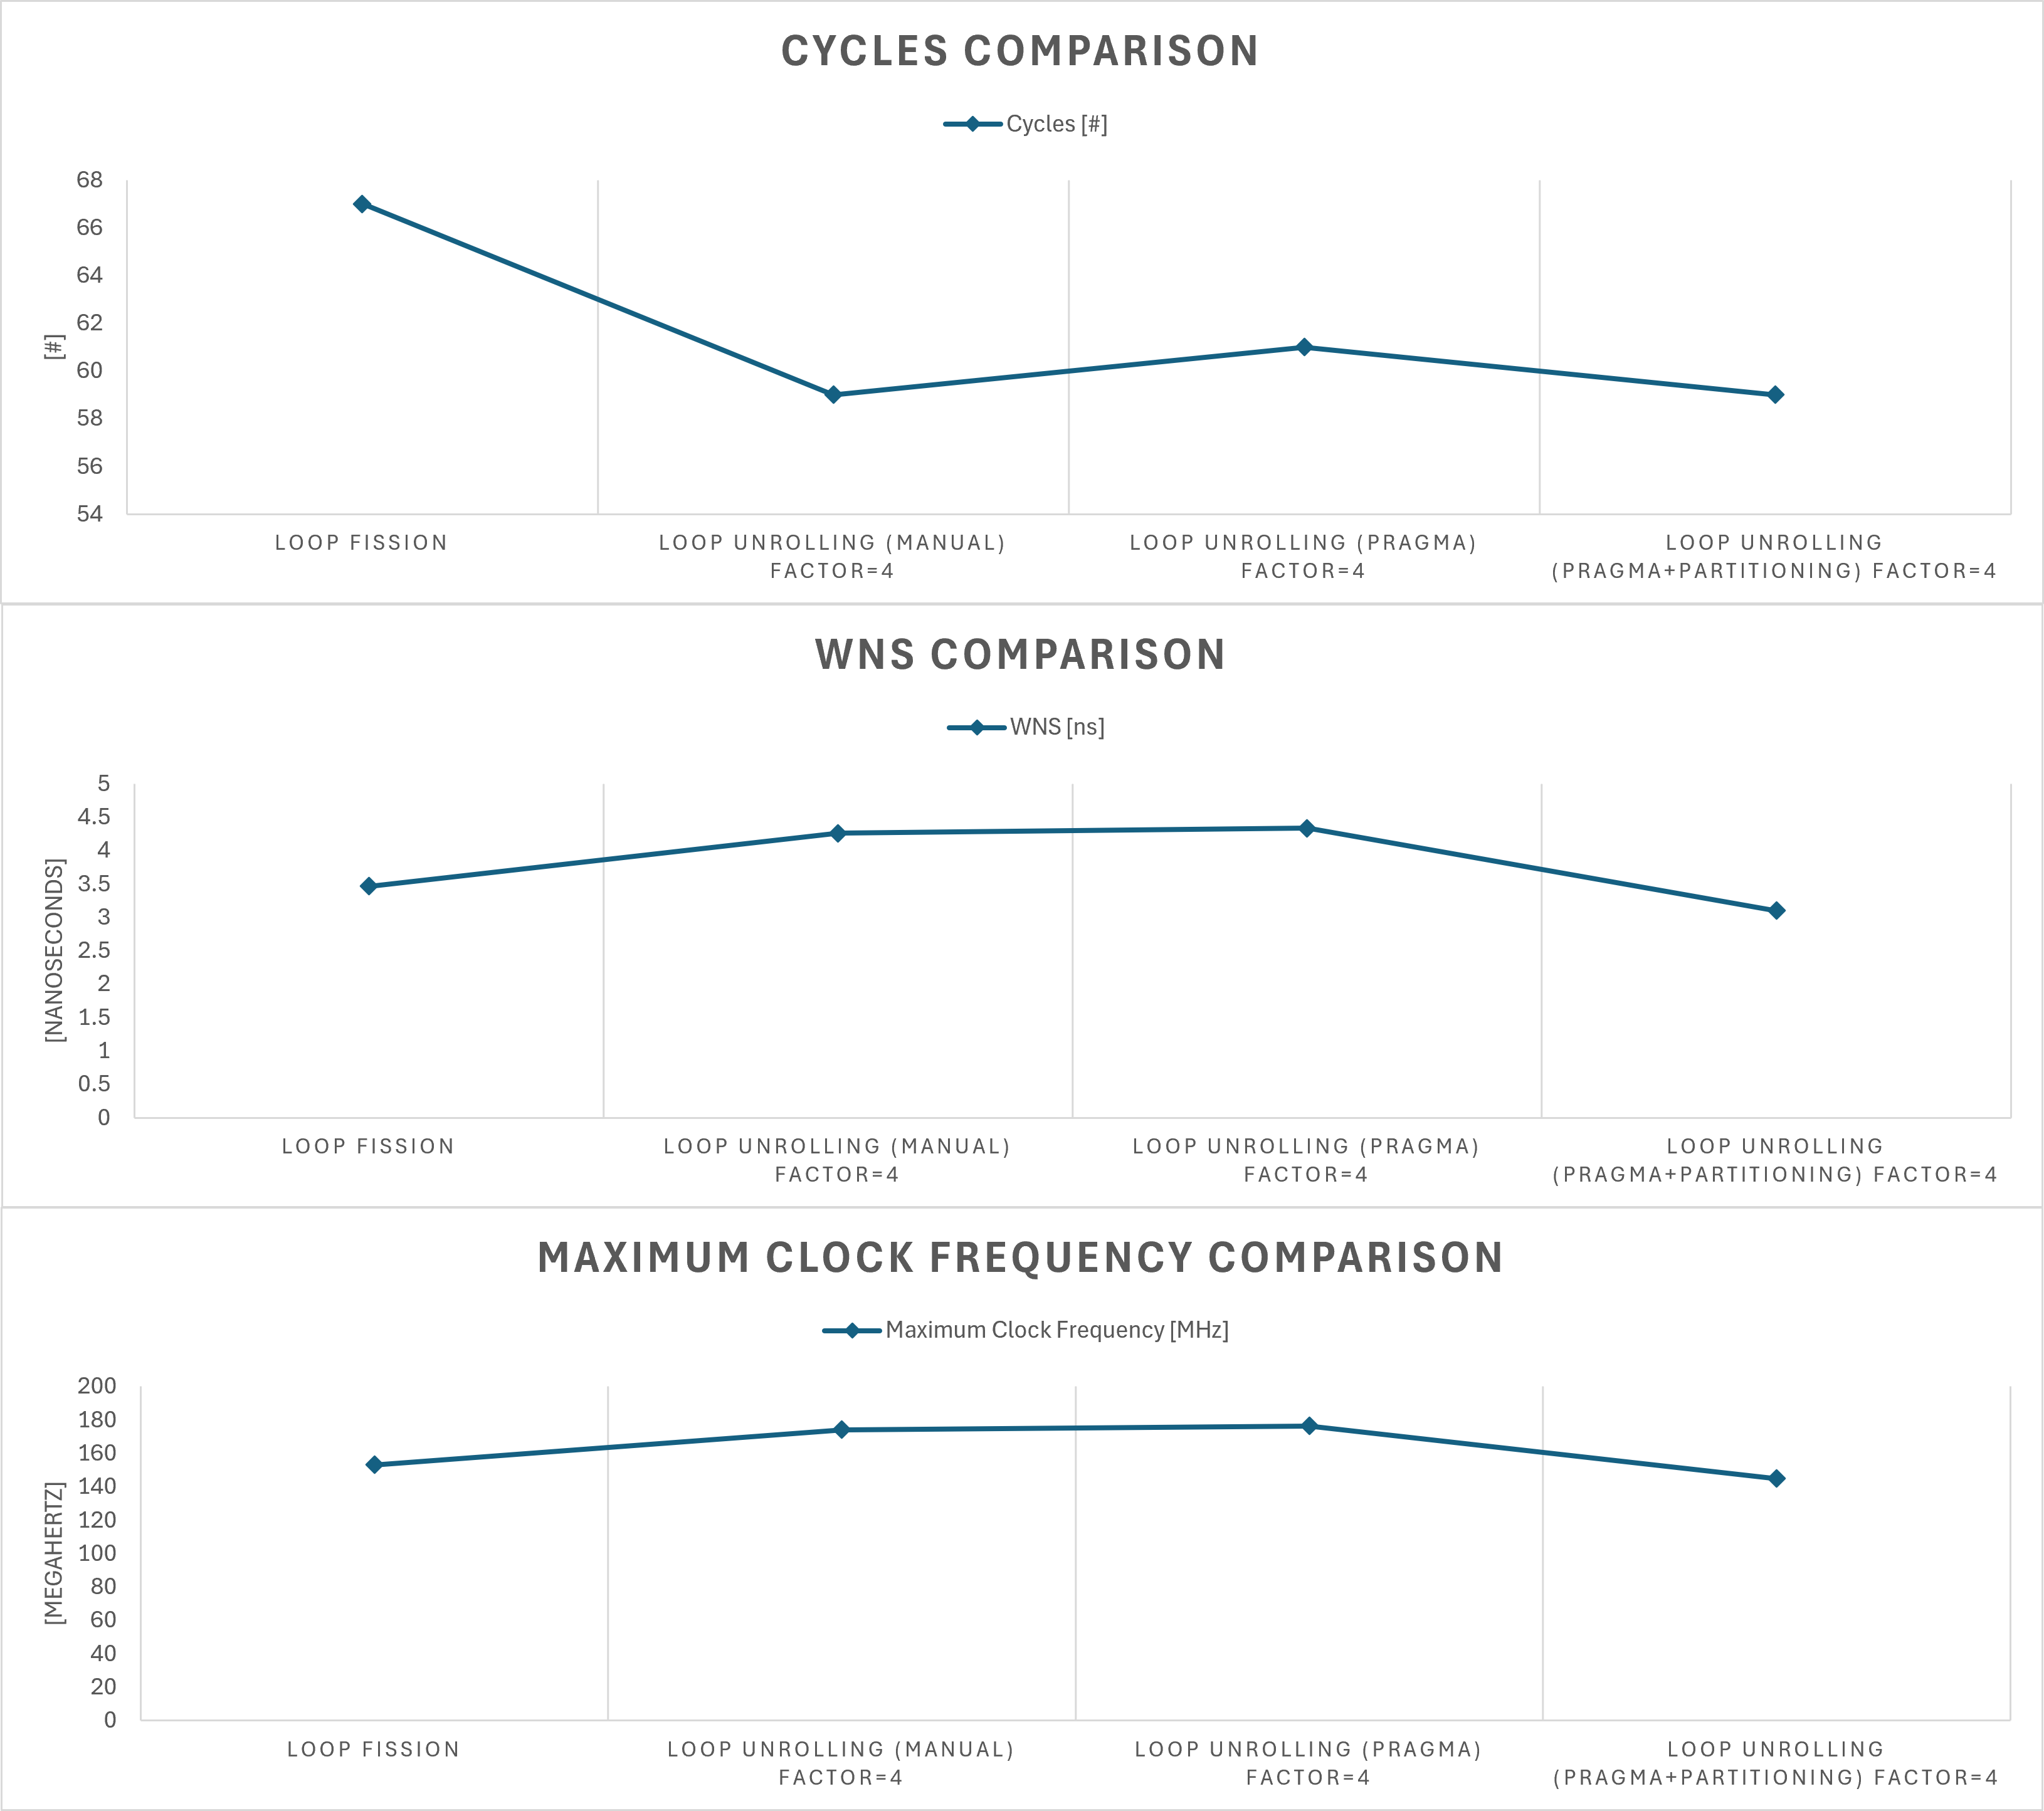
\includegraphics[width=0.8\textwidth]{solutions/loop_unrolling/factor4/loopunrollingfactor4timing.png}
    \caption{Vivado Loop Unrolling Factor=4 Timing Plot}
    \label{fig:vivado-loop-unrolling-factor4-solution-timing-plot}
\end{figure}

Analogamente all'unrolling di fattore pari a 2, anche in questo caso in corrispondenza della soluzione hardware basata su unrolling e partizionamento si ha un notevole aumento del contributo di potenza dinamica relativo al \textit{Clocks} comportando un aumento della potenza dinamica totale. 

\begin{table}[H]
    \centering
    \begin{tabular}{|c|c|c|c|c|c|c|c|}
        \hline
        \textbf{Solution} & \textbf{BRAM} & \textbf{Clock} & \textbf{Clocks} & \textbf{DSP} & \textbf{Logic} & \textbf{Set/}& \textbf{Data} \\
        & & \textbf{Enable} & & & & \textbf{Reset} & \\
        \hline
        Manuale & 1.32976193 & 0.382625905 & 0.253616716 & 0.921033497 & 0.543549308 & 0.010887122 & 0.585376518 \\
        \hline
        Automatico & 1.23103871 & 0.106978332 & 0.972227077 & 0.247065967 & 0.258892891 & 0.002585625 & 0.41881192 \\
        \hline
        Automatico & & & & & & & \\
        con & 0 & 0.328624592 & 2.560390625 & 0.298048515 & 1.146363211 & 0.0030065 & 1.324957004 \\
        Partitioning & & & & & & & \\
        \hline
    \end{tabular}
    \caption{Vivado Loop Unrolling Factor=4 Solution Dynamic Power Report [mW]}
    \label{tab:vivado-loop-unrolling-factor4-solution-dynamic-power-reproot}
\end{table}

\begin{table}[H]
    \centering
    \begin{minipage}[t]{0.45\linewidth}
        \centering
        \begin{tabular}{|c|c|}
            \hline
            \textbf{Solution} & \textbf{Dynamic Total} \\
            \hline
            Manuale & 4.026850996 \\
            \hline
            Automatico & 3.237600523 \\
            \hline
            Automatico & 5.661390447 \\
            con Partitioning & \\
            \hline
        \end{tabular}
        \caption{Vivado Loop Unrolling Factor=4 Solution Dynamic Power Report [mW]}
        \label{tab:vivado-loop-unrolling-factor4-solution-dynamic-power-reproot}
    \end{minipage}
    \hfill
    \centering
    \begin{minipage}[t]{0.45\linewidth}
        \centering
        \begin{tabular}{|c|c|}
            \hline
            \textbf{Solution} & \textbf{Energy Single Operation} \\
            \hline
            Manuale & 40.26850996 \\
            \hline
            Automatico & 32.37600523 \\
            \hline
            Automatico & 56.61390447 \\
            con Partitioning & \\
            \hline
        \end{tabular}
        \caption{Vivado Loop Unrolling Factor=4 Solution Energy Single Operation Report [pJ]}
        \label{tab:vivado-loop-unrolling-factor4-solution-solution-energy-single-operation-reproot}
    \end{minipage}
\end{table}

Bisogna notare un aspetto molto interessante. La potenza dinamica totale e l'energia per singola operazione associata alla soluzione hardware basata su loop unrolling automatico di fattore pari a 4 risultano essere pressocché le medesime di quelle relative all'unrolling automatico di fattore pari a 2. Questo potrebbe essere dovuto a ottimizzazione effettuate dal tool tramite la direttiva proprietaria dell'unrolling.

\newpage

\subsection{Loop Pipelining Solution}
Il pipelining consente di eseguire operazioni in modo simultaneo: ogni fase di esecuzione non deve completare tutte le operazioni prima di iniziare quella successiva. Pertanto, questo approccio permette di scindere le operazioni complesse in più operazioni semplici. In questo modo si può far lavorare l'architettura con dati temporalmente differenti. Ad esempio, tenendo conto della figura sotto allegata, questa funzione senza pipeline dovrebbe eseguire tutte le iterazioni previste in maniera sequenziale e, quindi, eseguendo read, compute, write, read, compute, write e così via. Considerando, invece, un approccio mediante pipeline, quello che succede è che alla prima iterazione viene eseguita la prima micro-operazione, alla seconda iterazione viene eseguita la seconda micro-operazione e in contemporanea si può eseguire la prima micro-operazione che nel caso precedente senza pipeline era prevista per il quarto ciclo di clock. L'idea è quella di far lavorare l'architettura sfruttando la scissione della logica complessa in più micro-operazioni. 

\begin{figure}[H]
    \centering
    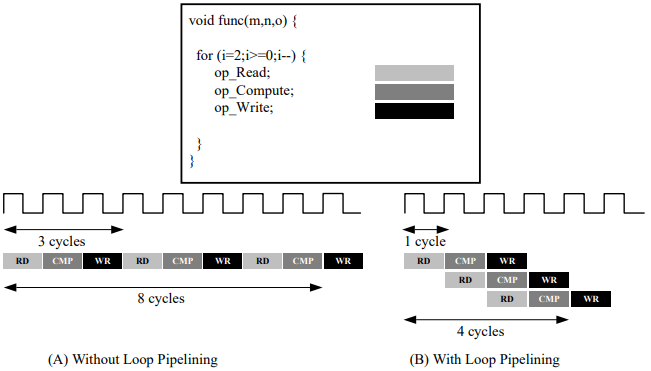
\includegraphics[width=1\textwidth]{solutions/loop_pipelining/looppipelining.png}
    \caption{HLS Loop Pipelining}
\end{figure}

In particolare, è possibile evidenziare due parametri fondamentali per questa tipologia di approccio:
\begin{itemize}
    \item \textbf{Iteration Latency (IL)}\\
    Numero di cicli che servono per eseguire un'iterazione del corpo del ciclo.
    \item \textbf{Initiation Interval (II) := Throughput}\\
    Numero di cicli di clock fino alla prossima iterazione del loop.
\end{itemize}

Idealmente, ci si aspetta un throughput pari a 1 perchè corrisponderebbe al caso migliore per il pipelining. Ovviamente non sempre è possibile ottenere un throughput pari a 1 ma in questo caso l'obiettivo è quello di ottenerlo.
\\
Il pipelining in HLS è possibile implementarlo mediante una direttiva proprietaria che permette, inoltre, di specificare l'Initiation Interval desiderato. Tanto è vero che all'interno del report di sintesi viene specificato l'II target, cioè quello specificato nella direttiva, e l'II raggiunto dal tool. Teoricamente, si dovrebbe ottenere II\_target=II\_achieved. Se così non fosse allora il tool non è riuscito a raggiungere l'obiettivo prefissato. Pertanto, si potrebbe modificare il codice per vedere se effettivamente il problema può essere risolto nella seguente maniera. Se così non fosse, evidentemente non dipende dal codice ma dal tipo di applicazione che si sta cercando di implementare che non lo permette.

\lstinputlisting[language=C++]{solutions/loop_pipelining/fir_loop_pipelining.cpp}

In questo caso, la soluzione hardware presa come riferimento è stata quella iniziale non ottimizzata. In particolare, all'interno del loop è stata definita sia la direttiva di pipeline, specificando un II=1, sia la direttiva di partizionamento. Nello specifico, è stato considerato il pragma di partitioning al fine di realizzabilità della soluzione in questione. Questo è dovuto al fatto che, senza considerare tale direttiva, si otterrebbe un II\_achieved differente da un II\_target. Infatti, utilizzare lo shift register vuol dire non poter accedere ai dati intermedi ma soltanto a quelli finali. Pertanto, per far fronte a questo problema si potrebbe pensare di realizzare tali shift register mediante Flip Flop (tramite la direttiva di partizionamento).
\\
Effettuando la sintesi otteniamo i seguenti report.

\begin{table}[H]
    \centering
    \begin{minipage}[t]{0.45\linewidth}
        \centering
        \begin{tabular}{|c|c|c|c|}
            \hline
            \textbf{Clock} & \textbf{Target} & \textbf{Estimated} & \textbf{Uncertainty} \\
            \hline
            ap\_clk & 10.00 & 8.510 & 1.25 \\
            \hline
        \end{tabular}
        \caption{HLS Loop Pipelining Solution Timing Summary (ns)}
        \label{tab:hls-loop-pipelining-solution-timing-summary}
    \end{minipage}
    \hfill
    \begin{minipage}[t]{0.45\linewidth}
        \centering
        \begin{tabular}{|c|c|c|c|}
            \hline
            \multicolumn{2}{|c|}{\textbf{Latency}} & \multicolumn{2}{|c|}{\textbf{Interval}} \\
            min & max & min & max \\
            \hline
            15 & 15 & 15 & 15 \\
            \hline
        \end{tabular}
        \caption{HLS Loop Pipelining Solution Latency Summary (clock cycles)}
        \label{tab:hls-loop-pipelining-solution-latency-summary}
    \end{minipage}
\end{table}

Si può notare come la latenza totale del loop sia notevolmente diminuita rispetto alla soluzione iniziale non ottimizzata. Inoltre, si può evidenziare come l'Initiation Interval raggiunto sia il medesimo di quello target, cioè pari a 1. Questo è stato possibile per i motivi precedentemente citati.
\\
In particolare, considerando il valore di Iteration Latency, il valore del Trip Count e il valore di Initiation Interval, è possibile ricavare il valore della latenza relativa al loop:
\begin{equation}
	IL+[(N-1)*II]-1 = 4+[(11-1)*1]-1 = 4+[10*1]-1 = 4+10-1 = 13	
\end{equation}

\begin{table}[H]
    \centering
    \begin{tabular}{|c|c|c|c|c|c|c|c|c|}
        \hline
        \multicolumn{1}{|c|}{Loop} & \multicolumn{2}{|c|}{\textbf{Latency}} & \multicolumn{2}{c|}{\textbf{Iteration Latency}} & \multicolumn{2}{c|}{\textbf{Initiation Interval}} & \multicolumn{1}{c|}{\textbf{Trip Count}}  \\
        Name & min & max & min & max & achieved & target &  \\
        \hline
        - loop & 13 & 13 & 4 & 4 & 1 & 1 & 11 \\
        \hline
    \end{tabular}
    \caption{HLS Loop Pipelining Solution Latency Loops Summary }
    \label{tab:hls-loop-pipelining-solution-loop-summary}
\end{table}

Per quanto riguarda l'utilizzazione stimata delle risorse, si può notare come il numero di FF sia aumentato rispetto alla soluzione non ottimizzata dal momento che è stato utilizzato il pragma di partizionamento tale da partizionare shiftRegister in diverse strutture da un certo numero di FF ciascuna anziché utilizzare BRAM.

\begin{table}[H]
    \centering
    \begin{tabular}{|l|c|c|c|c|}
        \hline
        \textbf{Name}    & \textbf{BRAM\_18K} & \textbf{DSP48E} & \textbf{FF} & \textbf{LUT} \\ \hline
        DSP              & -                   & -               & -           & -            \\ 
        Expression       & -                   & 4               & 0           & 480          \\ 
        FIFO             & -                   & -               & -           & -            \\ 
        Instance         & -                   & -               & -           & -            \\ 
        Memory           & 0                   & -               & 10          & 2            \\ 
        Multiplexer      & -                   & -               & -           & 75          \\ 
        Register         & -                   & -               & 700         & 64            \\ \hline
        \textbf{Total}   & 0                   & 4               & 710         & 621          \\ \hline
        \textbf{Available} & 280               & 220             & 106400      & 53200        \\ \hline
        \textbf{Utilization (\%)} & 0            & 1              & $\sim$0     & 1      \\ \hline
    \end{tabular}
    \caption{HLS Loop Pipelining Solution Utilization Estimates Summary}
    \label{tab:hls-loop-pipelining-solution-utilization-estimates-summary}
\end{table}

In particolare, si può notare come la direttiva proprietaria di partitioning ha partizionato shiftRegister in 10 strutture da 32 FF ciascuna.

\begin{table}[H]
	\centering
	\begin{tabular}{|l|r|r|r|r|}
		\hline
		\multicolumn{1}{|c|}{\textbf{Name}} & \multicolumn{1}{c|}{\textbf{FF}} & \multicolumn{1}{c|}{\textbf{LUT}} & \multicolumn{1}{c|}{\textbf{Bits}} & \multicolumn{1}{c|}{\textbf{Const Bits}} \\
		\hline
		accumulator\_reg\_114 & 32 & 0 & 32 & 0 \\
		ap\_CS\_fsm & 3 & 0 & 3 & 0 \\
		ap\_enable\_reg\_pp0\_iter0 & 1 & 0 & 1 & 0 \\
		ap\_enable\_reg\_pp0\_iter1 & 1 & 0 & 1 & 0 \\
		ap\_enable\_reg\_pp0\_iter2 & 1 & 0 & 1 & 0 \\
		ap\_enable\_reg\_pp0\_iter3 & 1 & 0 & 1 & 0 \\
		ap\_phi\_reg\_pp0\_iter1\_p\_pn\_reg\_138 & 32 & 0 & 32 & 0 \\
		ap\_phi\_reg\_pp0\_iter2\_p\_pn\_reg\_138 & 32 & 0 & 32 & 0 \\
		ap\_phi\_reg\_pp0\_iter3\_p\_pn\_reg\_138 & 32 & 0 & 32 & 0 \\
		coefficientsFilter1\_1\_reg\_458 & 10 & 0 & 10 & 0 \\
		i\_reg\_127 & 5 & 0 & 5 & 0 \\
		shiftRegister\_0 & 32 & 0 & 32 & 0 \\
		shiftRegister\_1 & 32 & 0 & 32 & 0 \\
		shiftRegister\_2 & 32 & 0 & 32 & 0 \\
		shiftRegister\_3 & 32 & 0 & 32 & 0 \\
		shiftRegister\_4 & 32 & 0 & 32 & 0 \\
		shiftRegister\_5 & 32 & 0 & 32 & 0 \\
		shiftRegister\_6 & 32 & 0 & 32 & 0 \\
		shiftRegister\_7 & 32 & 0 & 32 & 0 \\
		shiftRegister\_8 & 32 & 0 & 32 & 0 \\
		shiftRegister\_9 & 32 & 0 & 32 & 0 \\
		shiftRegister\_load\_p\_reg\_453 & 32 & 0 & 32 & 0 \\
		tmp\_1\_reg\_426 & 1 & 0 & 1 & 0 \\
		tmp\_2\_reg\_417 & 32 & 0 & 32 & 0 \\
		tmp\_4\_reg\_430 & 4 & 0 & 4 & 0 \\
		tmp\_6\_reg\_463 & 32 & 0 & 32 & 0 \\
		tmp\_reg\_422 & 1 & 0 & 1 & 0 \\
		tmp\_1\_reg\_426 & 64 & 32 & 1 & 0 \\
		tmp\_reg\_422 & 64 & 32 & 1 & 0 \\
		\hline
		Total & 700 & 64 & 574 & 0 \\
		\hline
	\end{tabular}
	\caption{HLS Loop Pipelining Solution Register Detail Estimates Summary}
	\label{tab:hls-loop-pipelining-solution-register-detail-estimates-summary}
\end{table}

Effettuando la C/RTL Cosimulation ed Export RTL si ottengono i seguenti report.

\begin{table}[H]
    \centering
    \begin{tabular}{|c|c|c|c|c|c|c|c|}
        \hline
        \multicolumn{1}{|c|}{RTL} & \multicolumn{1}{|c|}{Status} & \multicolumn{3}{c|}{\textbf{Latency}} & \multicolumn{3}{c|}{\textbf{Interval}} \\
        &  & min & avg & max & min & avg & max \\
        \hline
        VHDL & Pass & 15 & 15 & 16 & 15 & 15 & 16 \\
        \hline
    \end{tabular}
    \caption{HLS Loop Pipelining Solution C/RTL Cosimulation Summary }
    \label{tab:hls-loop-pipelining-solution-cosimulation-summary}
\end{table}

\begin{table}[H]
    \centering
    \begin{minipage}[t]{0.45\linewidth}
        \centering
        \begin{tabular}{|l|r|}
            \hline
            \textbf{Resource} & \textbf{VHDL} \\
            \hline
            SLICE & 204 \\
            \hline
            LUT & 311 \\
            \hline
            FF & 455 \\
            \hline
            DSP & 2 \\
            \hline
            BRAM & 0 \\
            \hline
            SRL & 0 \\
            \hline
        \end{tabular}
        \caption{HLS Loop Pipelining Solution Export RTL Resource Usage}
        \label{tab:hls-loop-pipelining-solution-export-rtl-resoruce-usage}
    \end{minipage}
    \hfill
    \begin{minipage}[t]{0.45\linewidth}
        \centering
        \begin{tabular}{|l|r|}
            \hline
            \textbf{Timing} & \textbf{VHDL} \\
            \hline
            CP required & 10.000 \\
            \hline
            CP achieved post-synthesis & 5.745 \\
            \hline
            CP achieved post-implementation & 6.512 \\
            \hline
        \end{tabular}
        \caption{HLS Loop Pipelining Solution Export RTL Final Timing}
        \label{tab:hls-loop-pipelining-solution-export-rtl-final-timing}
    \end{minipage}
\end{table}

Pertanto, importando l'IP in Vivado e impostando un clock constraint pari a 10ns è possibile analizzare i seguenti report di risorse, timing, potenza dinamica ed energia per singola operazione.
\lstinputlisting[language=VHDL]{solutions/loop_pipelining/clk_constraint.xdc}

Si può notare come, rispetto alla soluzione iniziale non ottimizzata, si è ottenuto un aumento di circa il $13\%$ delle LUT e un aumento di circa il $186\%$ dei FF.

\begin{table}[H]
    \centering
    \begin{tabular}{|c|c|c|c|c|c|c|}
        \hline
        \textbf{LUT} & \textbf{LUTRAM} & \textbf{FF} & \textbf{BRAM} & \textbf{DSP} & \textbf{IO} & \textbf{BUFG} \\
        \hline
        311 & 0 & 458 & 0 & 2 & 71 & 1 \\
        \hline
    \end{tabular}
    \caption{Vivado Loop Pipelining Solution Utilization Report [\#]}
    \label{tab:vivado-loop-pipelining-solution-utilization-report}
\end{table}

Inoltre, si può evidenziare come la maximum clock frequency sia aumentata di circa $15 MHz$ rispetto alla soluzione non ottimizzata di riferimento. Tanto è vero che il WNS, relativo alla soluzione realizzata mediante approccio di pipelining, risulta essere leggermente maggiore.

\begin{table}[H]
    \centering
    \begin{tabular}{|c|c|c|c|}
        \hline
        \textbf{Cycles} [\#] & \textbf{Clock Constraint} [ns] & \textbf{WNS} [ns] & \textbf{Maximum Clock Frequency} [Mhz] \\
        \hline
        16 & 10 & 4.208 & 172.6519337 \\
        \hline
    \end{tabular}
    \caption{Vivado Loop Pipelining Solution Timing Report}
    \label{tab:vivado-loop-pipelining-solution-timing-report}
\end{table}

In particolare, si può notare come, rispetto alla soluzione hardware iniziale non ottimizzata, i contributi di potenza dinamica sono aumentati tale da far aumentare l'energia per singola operazione. Nello specifico, si ha un aumento del contributo \textit{Clocks} di circa il $46\%$ dovuto principalmente all'aumento delle risorse associato alla solution in questione.

\begin{table}[H]
    \centering
    \begin{tabular}{|c|c|c|c|c|c|c|}
        \hline
        \textbf{BRAM} & \textbf{Clock Enable} & \textbf{Clocks} & \textbf{DSP} & \textbf{Logic} & \textbf{Set/Reset} [mW] & \textbf{Data} \\
        \hline
        0 & 0.196236724 & 1.778833685 & 0.814738101 & 1.275097136 & 0.012051522 & 1.206569896 \\
        \hline
    \end{tabular}
    \caption{Vivado Loop Pipelining Solution Dynamic Power Report [mW]}
    \label{tab:vivado-loop-pipelining-solution-dynamic-power-report}
\end{table}

\begin{table}[H]
    \centering
    \begin{minipage}[t]{0.45\linewidth}
        \centering
        \begin{tabular}{|c|}
            \hline
            \textbf{Dynamic Total} \\
            \hline
            5.283527065 \\
            \hline
        \end{tabular}
        \caption{Vivado Loop Pipelining Solution Dynamic Power Report [mW]}
        \label{tab:vivado-loop-pipelining-solution-total-dynamic-power-report}
    \end{minipage}
    \hfill
    \centering
    \begin{minipage}[t]{0.45\linewidth}
        \centering
        \begin{tabular}{|c|}
            \hline
            \textbf{Energy Single Operation} \\
            \hline
            52.83527065 \\
            \hline
        \end{tabular}
        \caption{Vivado Loop Pipelining Solution Energy Single Operation Report [pJ]}
        \label{tab:vivado-loop-pipelining-solution-energy-single-operation-report}
    \end{minipage}
\end{table}
\newpage

\subsection{Bitwidth Optimization Solution}
In questa sezione verrà discussa il possibile sovradimensionamento riguardo i tipi di dato relativi alle variabili utilizzate nelle varie architetture proposte. Effettivamente, nelle soluzioni hardware precedentemente citate, è stato principalmente utilizzato il tipo di dato \textit{int} anche in casi in cui bastava utilizzare un numero di bit notevolmente minore. Quello che si potrebbe fare è utilizzare tipi di dato aventi un numero di bit inferiore come, ad esempio, \textit{char} o \textit{short}. In alcuni casi, potrebbe accadere che il numero di bit richiesto è ulteriormente inferiore a questi tipi di dato disponibili negli ambienti \textit{C-like}. A tale proposito, nel contesto dei linguaggi ad alto livello C e C++, è disponibile una libreria, \textbf{ap\_int.h} che permette di modellare il tipo di dato \textit{int} scegliendo opportunamente il numero di bit da riservare per una determinata variabile. Pertanto, si potrebbe implementare una \textit{Bitwidth Optimization Solution} dove venga efficientemente allocato un numero di bit per le variabili al fine di ridurre l'utilizzazione delle risorse corrispondente. Ovviamente, utilizzare un numero ben preciso di bit per ogni variabile, vuol dire avere una soluzione custom per un certo range di bit e, nel caso in cui si debba utilizzare, ad esempio, un input che non sia incluso nel range di bit previsto, si dovrebbe, pertanto, implementare una nuova architettura con un numero di bit differente per le variabili corrispondenti. Ovviamente, in generale, si è considerato un numero di bit maggiorato di un'unità, dal momento che \textit{ap\_int.h} è una libreria che prevede un tipo di dato con segno.

\lstinputlisting[language=C++]{solutions/bitwidth_optimization/fir_bitwidth_optimization.cpp}

In particolare, la soluzione hardware proposta prevede un input ad 8 bit ed un output corrispondente a $18+SIZE = 18+11 = 29$ bit. La scelta del numero di bit relativi all'\textit{inputFilter} è arbitrario. Ovviamente, al variare di tale valore, il numero di bit previsto per le variabili interne cambierà di conseguenza. \\
Per quanto riguarda, invece, il numero di bit previsto per gli elementi presenti in \textit{coefficientsFilter}, sono stati considerati il valore massimo e minimo previsti all'interno dell'array. Riguardo l'array \textit{shiftRegister}, la bitwidth scelta è la medesima dell'input dal mommento che tale struttura dati viene utilizzata soltanto per lo shifting dei valori in ingresso all'architettura. Viceversa, la variabile \textit{accumulator} prevede un numero di bit uguale a quello dell'uscita del metodo. Infatti, tale variabile prevede, per ogni iterazione all'interno del ciclo for, una moltiplicazione e una somma. In particolare, la moltiplicazione richiede un numero di bit fisso, cioè 8+10 bit, mentre la somma, che viene effettuata sempre sulla medesima variabile in questione, richiede un numero di bit sempre maggiore per ogni iterazione. Quindi, tenendo conto che le iterazioni sono pari a $SIZE=11$, allora il numero di bit previsto per la variabile \textit{accumulator} è pari a $8+10+SIZE = 8+10+11 = 29$. Infine, per quanto riguarda il numero di bit associato alla variabile indice \textit{i} è relazionato al numero di iterazioni da effettuare che sono pari a $SIZE=11$.
\\
In particolare, l'architettura di riferimento utilizzata è basata sulla \textit{Code Hoisting Solution}. Pertanto, considerando i risultati ottenuti in corrispondenza della soluzione hardware citata ed effettuando la sintesi, la C/RTL Cosimulation e l'Export RTL della \textit{Bitwidth Optimization Solution}, è possibile effettuare i seguenti confronti.
\\
Si può notare come, dopo aver effettuato la sintesi, il numero di risorse, rispetto alla soluzione basata su Code Hoisting, presenti una diminuzione di circa il $65\%$ dei FF e di circa il $55\%$ delle LUT. Il numero dei DSP stimati è diminuito di 2 unità. Inoltre, si può notare come la latenza stimata è diminuita di 10 cicli rispetto alla soluzione presa come riferimento. Ovviamente il Trip Count è il medesimo dal momento che l'architettura proposta nella \textit{Bitwidth Optimization Solution} è equivalente a quella proposta nel \textit{Code Hoisting Solution}.

\begin{table}[H]
	\centering
	\begin{tabular}{|c|c|c|c|c|}
		\hline
		\textbf{Solution} & \textbf{Clock} & \textbf{Target} & \textbf{Estimated} & \textbf{Uncertainty} \\
		\hline
		Code Hoisting & ap\_clk & 10.00 & 8.510 & 1.25 \\
		\hline
		Bitwidth Opt. & ap\_clk & 10.00 & 6.38 & 1.25 \\
		\hline
	\end{tabular}
	\caption{HLS Bitwidth Optimization Solution Timing Summary (ns)}
	\label{tab:hls-bitwidth-optimization-solution-timing-summary}
\end{table}

\begin{table}[H]
	\centering
	\begin{tabular}{|c|c|c|c|c|}
		\hline
		\multicolumn{1}{|c|}{\textbf{Solution}} & \multicolumn{2}{|c|}{\textbf{Latency}} & \multicolumn{2}{|c|}{\textbf{Interval}} \\
		& min & max & min & max \\
		\hline
		Code Hoisting & 42 & 42 & 42 & 42 \\
		\hline
		Bitwidth Opt. & 31 & 31 & 31 & 31 \\
		\hline
	\end{tabular}
	\caption{HLS Bitwidth Optimization Solution Latency Summary (clock cycles)}
	\label{tab:hls-bitwidth-optimization-solution-latency-summary}
\end{table}

\begin{table}[H]
	\centering
	\begin{tabular}{|c|c|c|c|c|c|c|c|}
		\hline
		\multicolumn{1}{|c|}{\textbf{Solution}} & \multicolumn{1}{|c|}{Loop Name} & \multicolumn{2}{|c|}{\textbf{Latency}} & \multicolumn{1}{c|}{\textbf{Iteration Latency}} & \multicolumn{2}{c|}{\textbf{Initiation Interval}} & \multicolumn{1}{c|}{\textbf{Trip}}  \\
		&  & min & max & & achieved & target & \textbf{Count} \\
		\hline
		Code Hoisting & - loop & 40 & 40 & 4 & - & - & 10 \\
		\hline
		Bitwidth Opt. & - loop & 30 & 30 & 3 & - & - & 10 \\
		\hline
	\end{tabular}
	\caption{HLS Bitwidth Optimization Solution Latency Loops Summary }
	\label{tab:hls-bitwidth-optimization-solution-loop-summary}
\end{table}

\begin{table}[H]
	\centering
	\begin{tabular}{|c|c|c|c|c|}
		\hline
		\textbf{Solution} & \textbf{BRAM\_18K} & \textbf{DSP48E} & \textbf{FF} & \textbf{LUT} \\
		\hline
		Bitwidth Opt. & 0 & 4 & 230 & 240 \\
		\hline
		Code Hoisting & 0 & 2 & 81 & 107 \\
		\hline
	\end{tabular}
	\caption{HLS Bitwidth Optimization Solution Utilization Estimates [\#]}
	\label{tab:vivado-bitwidth-optimization-solution-utilization-report}
\end{table}

\begin{table}[H]
	\centering
	\begin{tabular}{|c|c|c|c|c|c|c|c|c|}
		\hline
		\multicolumn{1}{|c|}{\textbf{Solution}} & \multicolumn{1}{|c|}{RTL} & \multicolumn{1}{|c|}{Status} & \multicolumn{3}{c|}{\textbf{Latency}} & \multicolumn{3}{c|}{\textbf{Interval}} \\
		& &  & min & avg & max & min & avg & max \\
		\hline
		Code Hoisting & VHDL & Pass & 42 & 42 & 43 & 42 & 42 & 43 \\
		\hline
		Bitwidth Opt. & VHDL & Pass & 31 & 31 & 32 & 31 & 31 & 32 \\
		\hline
	\end{tabular}
	\caption{HLS Bitwidth Optimization Solution C/RTL Cosimulation Report }
	\label{tab:hls-bitwidth-optimization-solution-cosimulation-report}
\end{table}

Analizzando il report dell'Export RTL si può notare come l'utilizzazione delle risorse è notevolmente diminuita. Tanto è vero che il numero delle LUT e dei FF è diminuito di circa l'$82\%$. Questo decremento dell'utilizzazione delle risorse prevista è dovuto al fatto che nella \textit{Bitwidth Optimization Solution} sono stati utilizzati dei tipi di dato con un numero di bit custom per la soluzione in questione.

\begin{table}[H]
	\centering
	\begin{tabular}{|c|c|c|c|c|c|c|c|c|}
		\hline
		\textbf{Solution} & \textbf{SLICE} & \textbf{LUT} & \textbf{FF} & \textbf{DSP} & \textbf{BRAM} & \textbf{CP} & \textbf{CP} & \textbf{CP} \\
		& & & & & & \textbf{required} & \textbf{achieved} & \textbf{achieved}\\
		& & & & & & & \textbf{post-} & \textbf{post-}\\
		& & & & & & & \textbf{synthesis} & \textbf{implementation}\\
		\hline
		Code Hoisting & 75 & 270 & 131 & 2 & 0 & 10 & 5.745 & 6.847 \\
		\hline
		Bitwidth Opt. & 15 & 50 & 24 & 2 & 0 & 10 & 5.745 & 5.692 \\
		\hline
	\end{tabular}
	\caption{HLS Bitwidth Optimization Solution Export RTL Report}
	\label{tab:vivado-bitwidth-optimization-solution-export-rtl-report}
\end{table}
